%!!!!!!!!!!!!!!!!!!!!!!!!!!!!!!!!!!!!!!!!!!!!!!!!!!!!!!!!!!!!!!!!!!!!!!!!!!!!!!
%!NOTE: This example file has been prepared according to the University of
%!      Hawaii Style & Policy Manual for Theses and Dissertations dated
%!      "Revised September 2010". If you have one with a later date, you may
%!      need to make revisions to this document as well. In any event, making
%!      sure your thesis complies with Graduate Education guidelines is
%!      ultimately your responsibility. Caveat LaTeXtor. :)
%!!!!!!!!!!!!!!!!!!!!!!!!!!!!!!!!!!!!!!!!!!!!!!!!!!!!!!!!!!!!!!!!!!!!!!!!!!!!!!

%% The options are (you can only choose one from each group):
%%
%% 10pt, 11pt, 12pt: chooses the point size for the document. "11pt" is the
%%                   default.
%%
%% oneside, twoside: whether you want your document onesided or twosided. Note
%%                   that twosided is not guaranteed to work, and style
%%                   guidelines prohibit double sided printouts on final
%%                   copy. "oneside" is the default.
%%
%% draft, final: when printing drafts you can save a lot of paper by using the
%%               "draft" option. It switches to single spacing, displays overful
%%               hboxes with a black box, prints a version number on title page 
%%               and omits signature page. Of course for the final copy make
%%               sure to use the "final" option! "final" is the default.
%%
%% thesis, dissertation: switches between the style for a master's thesis and a 
%%                       Ph.D. dissertation. The differences are fairly minor
%%                       and limited to the front matter. "thesis" is the
%%                       default.
%%
%% actual, proposal: switches between actual document and proposal mode. In
%%                   proposal mode: the title page is simplified and the
%%                   version number is always printed.
%%
%%% Load the new uhthesis document class

\documentclass[11pt, thesis, actual]{uhthesis}
\setcounter{secnumdepth}{5}
%%% Load some useful packages:
%% New LaTeX2e graphics support
\usepackage{graphicx}
\PassOptionsToPackage{hyphens}{url}\usepackage{hyperref}
\graphicspath{ {images/} }
%% Package to linebreak URLs in a sane manner.
\usepackage{url}
\usepackage{verbatim}
\usepackage{array,tabularx}
\usepackage{subcaption}
%%% Declarations for Front Matter. Capitalize all of these values
%%% "normally". This allows the document class to format them properly.
%% Full title of \textbf{}thesis or dissertation, capitalized like a title should be.
\title{RADGRAD: Improving Academic, Professional, and Social Engagement During the Undergraduate Computer Science Degree Experience}
%% Your name, capitalized normally. Do not include any titles like Dr.
\author{Amy M. Takayesu}
%% Month in which you intend to receive your degree (i.e. graduation).
%% Presumably this will be one of: May, August, or December.
\degreemonth{August}
%% Year of expected graduation.
\degreeyear{2017}
%% Type of degree to be conferred.
\degree{Master of Science}
%% This is the chairperson of your committee. Do not use titles like Dr.
\chair{Philip M Johnson}
%% The other members of your committee, seperated by "\\". Again, no titles,
%% and it is customary to list the outside committee member (if you have one)
%% last.
\othermembers{Dan Suthers\\Michael-Brian Ogawa}
%% The field in which you are obtaining your degree, capitalized normally.
\field{Computer Science}
%% If your discipline allows subfields, you can add it here. Note that this
%% is strictly controlled, so consult the Style & Policy guide before adding
%% a subfield.
%\subfield{Bioinformatics}
%% 4-6 optional keywords/phrases for use in indexing or as search terms
\keywords{Software Development, Educational Technology, Social Network, Degree Planner, Gamification}
%% The version number of your document. Consistent use of this will enable you
%% to tell old drafts from new ones. Final actual documents omit this
%% automatically so you can use it without fear of submission problems at the
%% end. If you do not define this parameter, it defaults to "1.0.0".

%%% End of preamble
\begin{document}
\maketitle
\begin{frontmatter}

%%% Note, there is no longer a signature page included in the document, it
%%% has been replaced by Form IV

%%% Create the copyright page (optional)
\copyrightpage

%%% Bring in the dedication page from external file (optional)
%%%% \include{dedication}

%%% Bring in the acknowledgments section from external file (optional)
%%%% %%%%%%%%%%%%%%%%%%%%%%%%%%%%%% -*- Mode: Latex -*- %%%%%%%%%%%%%%%%%%%%%%%%%%%%
%% uhtest-acknowledgements.tex -- 
%% Author          : Robert Brewer
%% Created On      : Fri Oct  2 16:29:43 1998
%% Last Modified By: Robert Brewer
%% Last Modified On: Fri Oct  2 16:29:52 1998
%% RCS: $Id: uhtest-acknowledgements.tex,v 1.1 1998/10/06 02:06:54 rbrewer Exp $
%%%%%%%%%%%%%%%%%%%%%%%%%%%%%%%%%%%%%%%%%%%%%%%%%%%%%%%%%%%%%%%%%%%%%%%%%%%%%%%
%%   Copyright (C) 1998 Robert Brewer
%%%%%%%%%%%%%%%%%%%%%%%%%%%%%%%%%%%%%%%%%%%%%%%%%%%%%%%%%%%%%%%%%%%%%%%%%%%%%%%
%% 

\begin{acknowledgments}

First, I would like to thank Prof. Philip Johnson for his endless enthusiasm, positive energy, and wisdom, which enabled me to complete my thesis within a year with minimum pain. Next, I would like to thank Prof. Dan Suthers and Prof. Michael Brian Ogawa for being on my committee and being patient with me as I attempted to organize my thesis both in my head and on paper. I would also like to thank Prof. Cam Moore for patiently providing me with his RadGrad advice and life wisdom during the past year. I would also like to thank Josephine Garces and Aljon Preza for their selfless contributions to the RadGrad development. Additionally, I would like to thank the Collaborative Software Development Laboratory (CSDL) for providing me with an office with a window. Finally, I would like to thank Gerald Lau for letting me sit in his office and talk to him about spaghetti for an entire month. 

\end{acknowledgments}


%%% Bring in the abstract section from external file
 \begin{abstract}

A casual analysis of the Hawaii technology community site, TechHui, suggests that over the past decade, recent alumni and current undergraduates have experienced several problems with various academic, professional, and social aspects of their ICS experience. A baseline student survey conducted in Spring 2017 reveals current and more detailed student perceptions on the ICS degree experience. Existing degree planning systems such as STAR, Starfish by Hobsons and Blackboard Planner fail to provide the specific support that an ICS student needs to create a complete and comprehensive degree plan. Existing academic social networks such as LinkedIn and TechHui fail to connect students closely with professors and alumni. Current popular video games suggest several gamification features that could encourage ICS students to achieve higher goals. A new system called RadGrad combines degree planning, social networking, and gamification in a way that aims to give ICS undergraduates the support they need to succeed and redefines what it means to have a successful degree experience.
\end{abstract}


%%% Generate table of contents
\tableofcontents

%%% Generate list of tables
%%% \listoftables

%%% Generate list of figures
%%%\listoffigures

\end{frontmatter}

%\normalsize
%%% Bring in the body of the thesis from external file
\chapter{Introduction}
\label{introduction}

Getting a college degree is an investment that many people make, with the expectation that once they get their degree, they will have the basic skills needed to start a career in the field of their choice. However, what happens if a student does everything they are told to do (takes required courses, gets a high GPA, and graduates on time), but once they start applying for jobs, they are constantly turned down and told that their coursework and high GPA are not enough? If colleges promise to prepare students for the workforce, they should be doing everything they can do deliver this promise, even if it means redefining what it means for a student to be "successful."   

For ICS students in 2017, it is hard to land a job when the only thing on your resume is a couple of standard programming courses and 3.8 GPA. Several ICS alumni have told me that they realized too late that employers are scouring incoming resumes for other things like internships, independent projects, and hackathons. It is also difficult for ICS students to find jobs in new industries that may not have existed, or may have been far less prominent four years ago when they began their ICS degree. How can these students prepare for these new fields, when they had no concept of it during their degree experience? Furthermore, is it reasonable to expect colleges to create new courses each time there is an advancement in technology?

These initial observations made me wonder if other ICS students over past decade were experiencing similar problems. To answer this question, I navigated to the Hawaii technology community site, TechHui \cite {TechHuiQuestions}, and found a forum question entitled "Three bad things about being an ICS student." I gathered responses from 199 ICS students from 2008 to 2016, and compiled a list of the ten most common complaints over the past 8 years:

\begin{enumerate}
  \item The ICS department needs to offer classes more frequently.
  \item The ICS department needs to offer a wider variety of classes.
  \item The ICS department needs a better sense of community.
  \item Some of the professors in the ICS department need to improve their teaching.
  \item The ICS department should offer more focused areas of study.
  \item ICS classes are too time consuming and take up more time than anticipated.
  \item The ICS department should offer more classes that meet focus requirements.
  \item ICS books are too expensive.
  \item ICS courses should involve more group work 
  \item ICS should encourage more interaction among students.
\end{enumerate}

Complaints 1, 2, 5, 6, 7, and 8 suggest problems with degree planning and coursework itself and complaints 3, 4, 9, and 10 suggest social and communication related problems within the department. There were also some other complaints among students on TechHui that were not as common but stuck out to me nonetheless. There were at least eight students who mentioned that they felt intimidated when they started out in ICS, due to the impressions they got from their classmates and the major overall. This caused them to feel discouraged and had an overall negative impact on their ICS experience. These sentiments further suggest social problems with the ICS community, as well as with how the department is perceived outside of the community. 

As ideal as it would be, it is hard to meet the needs of all current, past and present students in a department. However, after taking student and alumni feedback into consideration, several of these problems could potentially be alleviated by creating an online platform that provides students with the help they need to become a truly successful student--academically, professionally, and socially. Creating a useful degree planner that helps students get all the information they need to create an ideal plan for their personal goals could help students academically. Creating an online social network for the ICS community could help encourage students to connect with others in the department. Adding gamification aspects to the degree experience could help give students extra incentives to go beyond the UHM graduation requirements, and take the initiative to become more well prepared for finding a job after graduation. By combining these three components (degree planner, social network, and gamification), a new system called RadGrad could potentially address many of the aforementioned student problems and needs.  


\chapter{Related Work}
\label{related-work}

My vision of addressing ICS student problems through an online platform involves three major parts: degree planner, social network, and gamification. All three of these parts combine to create a robust, interactive, and effective system to enhance the academic journeys of current and future ICS students. In this section I discuss existing software in each of these categories, what they aim to accomplish, and why they do not fully satisfy the needs of ICS students.

\section{Degree Planners}
\begin{figure}[h]
\centering

\includegraphics[width=0.5\textwidth]{star_home}
\caption{STAR homepage. \textit{Source: www.star.hawaii.edu}}
\label{star-home}
\end{figure}
\subsection{STAR}

STAR is the degree planning system currently used by the University of Hawaii system \cite{STAR} (Figure ~\ref{star-home}). As of June 2017, the student interface provides five main capabilities: Academic Essentials, Graduation Pathway, What If Journey, Transcripts, and Scholarships. 

\begin{figure}[h]
\centering
\includegraphics[width=0.5\textwidth]{star_edgoals}
\caption{STAR Academic Essentials page. \textit{Source: www.star.hawaii.edu}}
\label{star-edgoals}
\end{figure}
\subsubsection{Academic Essentials}

This interface provides information about the student's academic progress, and compares it to the student's academic requirements to show the student's progress towards graduation (Figure ~\ref{star-edgoals}). This information includes credit totals, grades, and required courses. This interface also includes a section for ``Advisor Notes", which is filled out during advising sessions. There is another section for ``Events and Actions" which lists important student academic events such as college applications, admittance, and graduation, and student academic actions such as Deans List award. A third section is called ``Educational Goals", which provides the student's ``immediate goals" and ``highest ed goals" on a semester-by-semester basis. This information is provided by the student through occasional assessments upon log-in to STAR. The top of the page also has a section for students with financial aid.

\begin{figure}[h]
\centering
\includegraphics[width=0.5\textwidth]{star_pathway}
\caption{STAR Academic Graduation Pathway page.\textit{Source: www.star.hawaii.edu}}
\label{star-pathway}
\end{figure}

\subsubsection{Graduation Pathway}

This interface is provided for certain programs or exploratory or pre-major students (Figure ~\ref{star-pathway}). It displays the course information for the courses that the student has taken previously and is currently enrolled in, and shows which requirements each course fulfills. It also lets students view future semesters and suggests future types of classes that the student should enroll in, in order to fulfill their major requirements. This interface does not suggest specific classes, but only lists the requirement that the class will need to fulfill. 

\begin{figure}[h]
\centering
\includegraphics[width=0.5\textwidth]{star_whatif}
\caption{STAR What If page. \textit{Source: www.star.hawaii.edu}}
\label{star-what-if}
\end{figure}

\subsubsection{What If Journey}

This interface is provided for undergraduates at UH Manoa. It allows students to choose a different major than their current one (Figure ~\ref{star-what-if}), and shows an altered version of their STAR homepage, which displays the requirements of the chosen major. This helps students visualize where they would be in the program if they were to switch majors.

\begin{figure}[h]
\centering
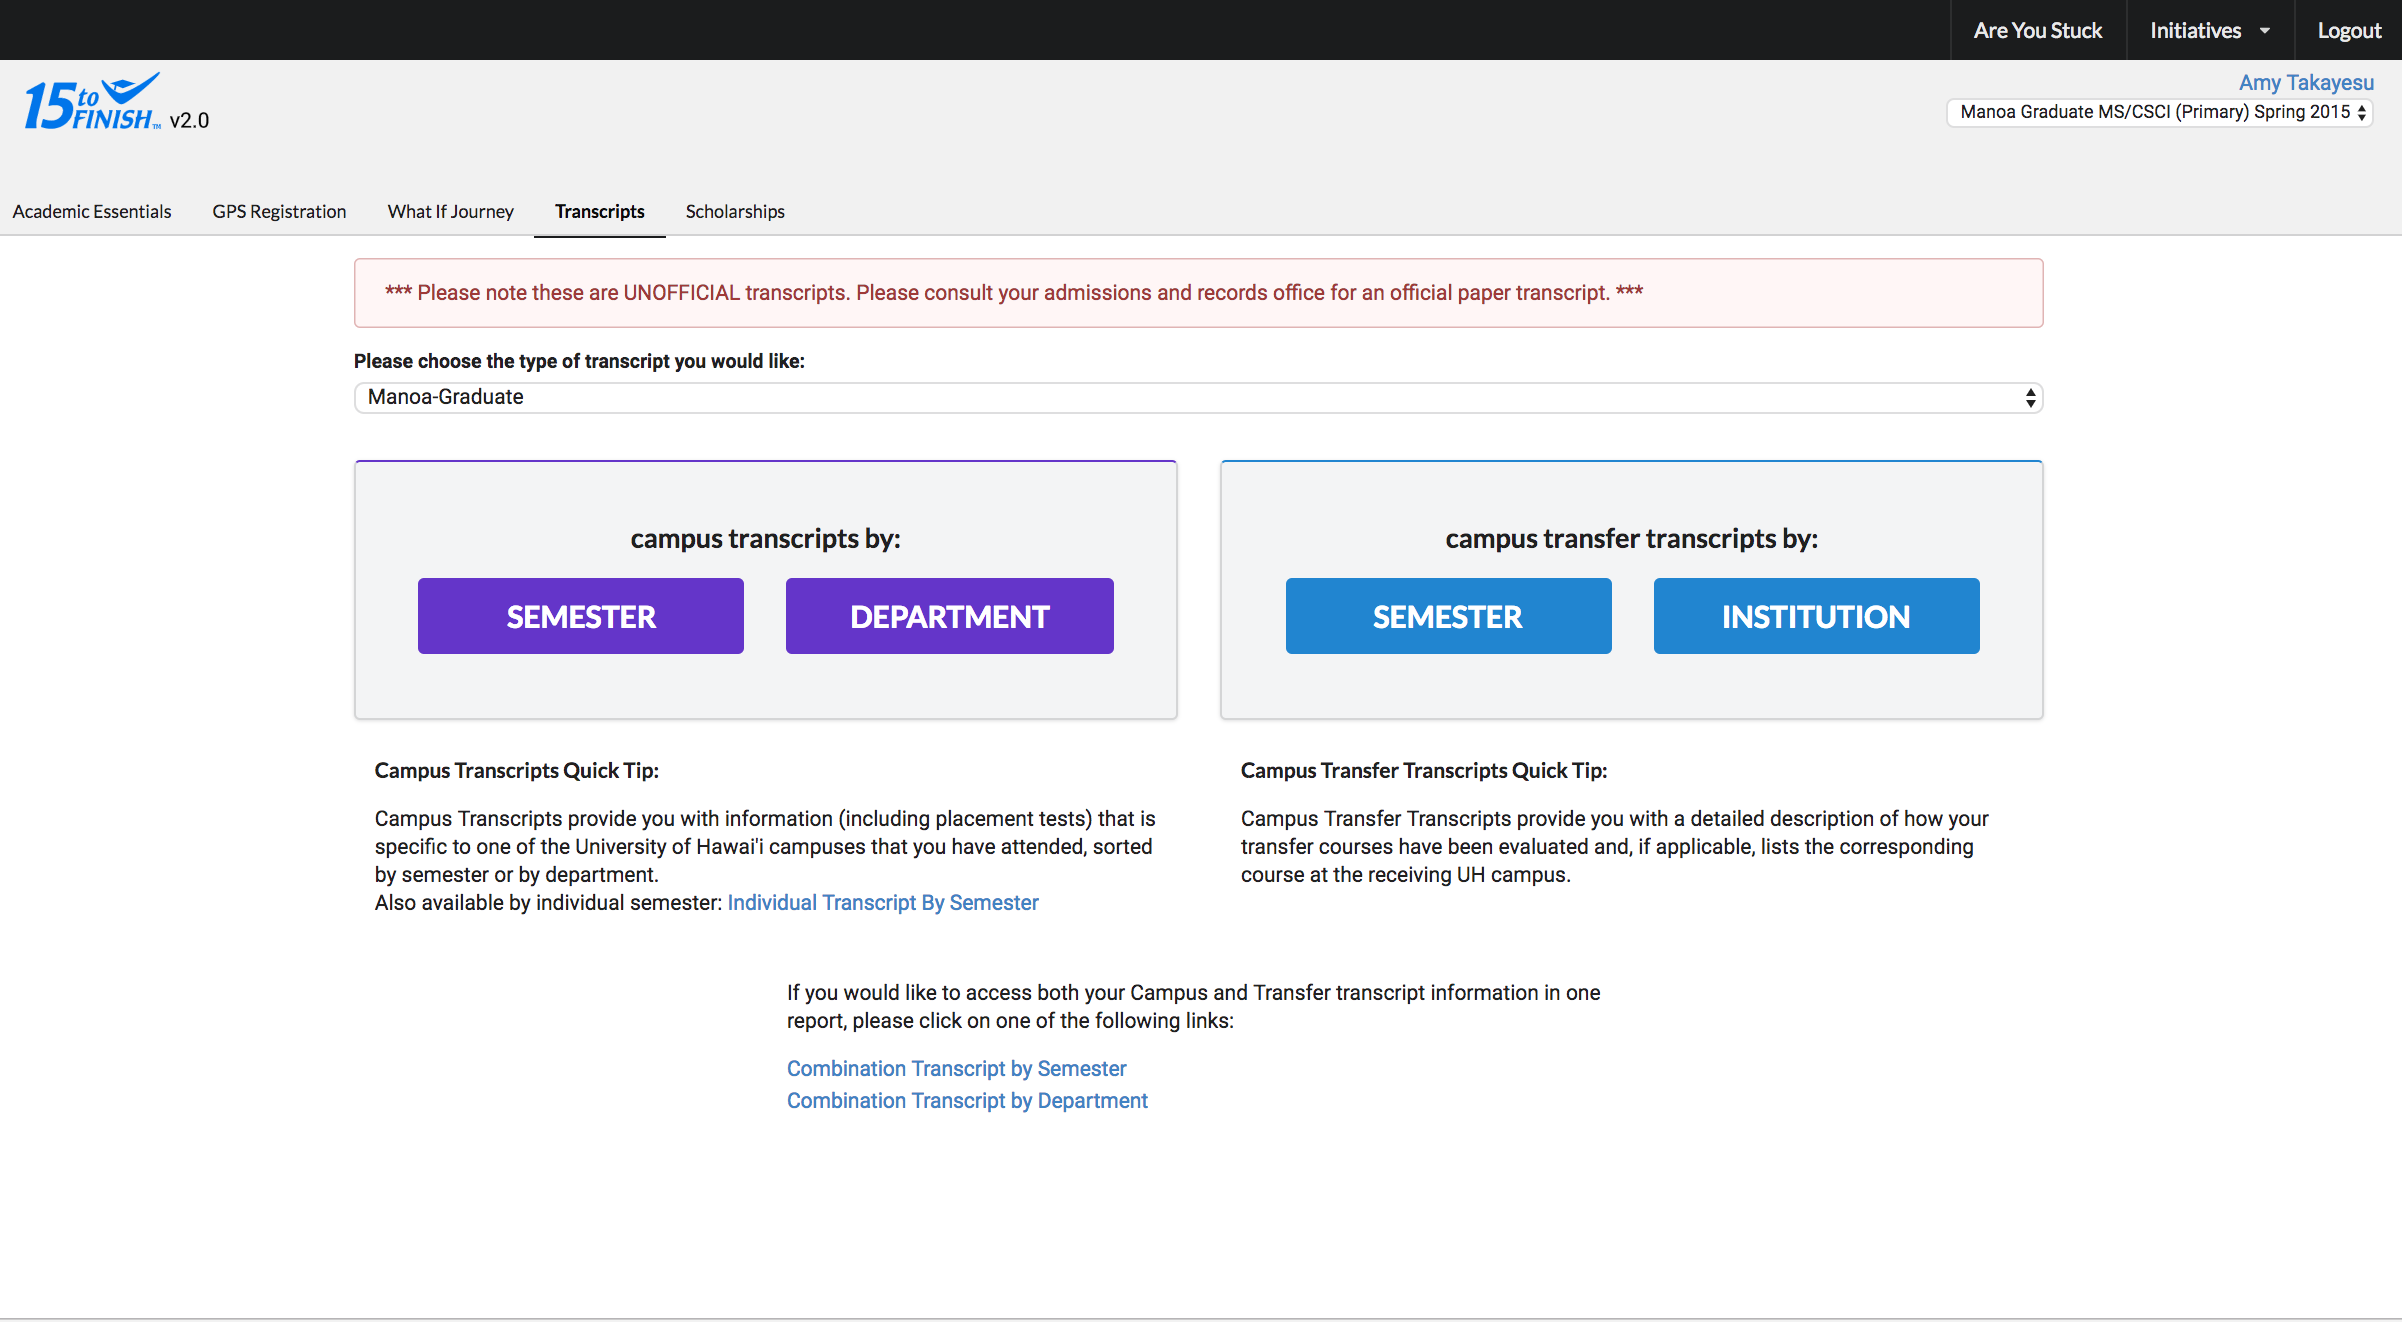
\includegraphics[width=0.5\textwidth]{star_trans}
\caption{STAR Transcripts page. \textit{Source: www.star.hawaii.edu}}
\label{star-transcripts}
\end{figure}

\subsubsection{Transcripts}

This interface allows students to access their campus transcripts by semester and by department (Figure ~\ref{star-transcripts}). It also allows transfer students to access their transfer transcripts by semester and by institution. 
\begin{figure}[h]
\centering
\includegraphics[width=0.5\textwidth]{star_scholar2}
\caption{STAR Academic Scholarship Home page. \textit{Source: www.star.hawaii.edu}}
\label{star-scholarship-home}
\end{figure}
\begin{figure}[h]
\centering
\includegraphics[width=0.5\textwidth]{star_scholar3}
\caption{STAR Academic Scholarship Best Fit page. \textit{Source: www.star.hawaii.edu}}
\label{star-scholarship-best-fit}
\end{figure}
\begin{figure}[h]
\centering
\includegraphics[width=0.5\textwidth]{star_scholar4}
\caption{STAR Academic Scholarship Keyword Search page. \textit{Source: www.star.hawaii.edu}}
\label{star-scholarship-keyword}
\end{figure}
\subsubsection{Scholarships}

This interface allows students to find scholarships by either using a keyword search or by selecting the ``My Best Fit Scholarship" tab, which presumably gathers student academic data and compares it with scholarship data to find matches (Figure ~\ref{star-scholarship-home}, Figure ~\ref{star-scholarship-best-fit}, Figure ~\ref{star-scholarship-keyword}).

\subsubsection{STAR and Academic/Professional/Social Engagement}

STAR is the all-in-one place for UH students to check on their progress in general education and major courses, University status in terms of enrollment and tuition payment, and their official transcripts. Since STAR is designed to fit the general academic needs of all students at UH, it is unrealistic to expect STAR to provide specialized and detailed support for each department. Each department is different in terms of courses and requirements, and STAR does not offer any features that go into depth in each individual department's idiosyncrasies. To get more detailed information about major requirements, students must access separate department websites or contact the department's academic adviser. 
In features such as Academic Essentials, Graduation Pathway, and Scholarships, STAR only offers baseline information. For instance, in Academic Essentials, STAR focuses on the student's broad academic goals (e.g. graduation date and highest degree goal) rather than their arguably more helpful and specific major-related goals. In Graduation Pathway, STAR notifies students which course categories they are missing, but does not suggest the specific classes that they are missing. In Scholarships, STAR lists relevant scholarships but does not provide detailed information about how to apply or how to prepare for them. Although STAR succeeds at being a University-wide, cross-departmental degree planner system, it lacks the detailed department-specific support that is crucial for a student's success and growth within his/her major. 

\begin{figure}[h]
\centering
\includegraphics[width=0.5\textwidth]{starfish_connect}
\caption{Example Starfish Connect page. \textit{Source: Starfish CONNECT gallery}}
\label{starfish-connect}
\end{figure}
\subsection{Starfish by Hobsons}

The slogan for Hobsons is ``Education Advances: Imagine a world where all students find their best fit \cite{Starfish}." Hobsons offers a wide range of educational solutions, ranging from students K-12 to college students. Starfish by Hobsons is one of their platforms which focuses on success, support, and retention initiatives, and engaging students more effectively with the campus community. There are three main parts of the Starfish Enterprise Success System: Early Alert, Connect, and Degree Planner.

\subsubsection{Early Alert}

Early Alert is a early warning and student tracking model which mines student performance data from existing technologies at the particular institution to detect at-risk students. These students are detected early enough, such as at the first sign of a problem, so that there is enough time to make a difference. There is a type of reward system called Kudo (a positive feedback note), which is used to encourage students and reward them for improvement or good work. 

\subsubsection{Connect}

Connect is an online appointment scheduling and case management system (Figure ~\ref{starfish-connect}). This system promotes communication between students and their advisers, instructors, and tutors by means of in person meetings, phone calls, or virtual meetings. Connect includes a kiosk to allow easily scheduled walk-in meetings. These kiosks can help staff to manage a student queue and also allows students to check wait times remotely, which can save a lot of time and frustration. Connect also includes a road map for each student, which documents the steps a student must take to achieve his or her goals. This map is created by an adviser and is visible to all members of the student's support network. 

\subsubsection{Degree Planner}

Degree Planner provides academic templates which advisers can use to easily edit to adjust to a particular student's needs. It also focuses on students' constantly changing goals and ability to adjust the student's plan to accommodate these goals. When a student deviates from their given plan, the student's adviser is notified so that they can plan a meeting with the student to check on their status and re-identify their goals. 

\subsubsection{Starfish by Hobsons and Academic/Professional/Social Engagement}

Starfish by Hobsons provides integrated systems that can keep track of students and keep students on track \cite{Starfish}. Its integration into different departments and customization of more specific goals fulfills the academic goals of RadGrad more than STAR. However, this system is concerned only with academics and does not take other factors into consideration such as internships, outside work and projects, and other extracurricular activities. While a student may seem to be on track based off their academic record, there are other factors that come into play when it comes to ``staying on track." Traditionally, an ``on track" student may have completed all of the coursework within 4 years with at least a 3.0 GPA. However, what if ``on track" were redefined to be much more complex, and include other factors outside of coursework? Although these factors may not technically be requirements to graduate, they may be highly recommended, and a system that could help encourage students to pursue these other factors, without them being technically required, would create a different class of graduates entirely. 

\subsection{College Scheduler}

The College Scheduler company has two products: Schedule Planner and Pathway Planner  \cite{CollegeScheduler}. The Schedule Planner focuses on optimizing the way students can plan their schedules, and the Pathway Planner focuses on optimizing the way students progress towards graduation.

\begin{figure}[h]
\centering
\includegraphics[width=0.5\textwidth]{college_sched_sp}
\caption{Example of Schedule Planner. \textit{Source: http://www.collegescheduler.com/schedule-planner/}}
\label{college-sched}
\end{figure}

\subsubsection{Schedule Planner}

Schedule Planner allows students to easily schedule (or automatically generate) their classes around outside obligations (Figure ~\ref{college-sched}). It also helps students to maximize their credit hours and graduate on time. Schedule Planner also analyzes student preference data to predict the optimal number of course sections to offer and helps to evenly distribute class fill rates. It enables advisers to create course schedules for groups of students at a time. One of their main goals is to allow students to focus on which courses to take rather than worrying about when they are being offered.

\begin{figure}[h]
\centering
\includegraphics[width=0.5\textwidth]{college_sched_pp}
\caption{Example of Pathway Planner. \textit{Source: http://www.collegescheduler.com/pathway-planner/}}
\label{pathway-planner}
\end{figure}

\subsubsection{Pathway Planner}

The Pathway Planner allows students to plan their schedules in a multi-year format to encourage seeing the bigger picture and to plan ahead (Figure ~\ref{pathway-planner}). It provides visuals to show students how their predicted course loads will affect their graduation date. Administrators can also see the courses that students plan on taking before registration. This allows for the addition and elimination of courses to best fit student needs. 

\subsubsection{College Scheduler and Academic/Professional/Social Engagement}

College Scheduler focuses on the scheduling aspect of degree planning. However, it views scheduling as a long term event, and allows students and administrators to work together to offer courses in an optimal manner. While College Scheduler addresses the needs to students as a whole, it does not offer individualized support based off individual needs. Every student has different goals, plans, and schedules, and there is no one master schedule that can accommodate them all. However, if it were to offer individual support on a case by case basis, it would be able to help a larger amount of students to reach their unique goals. 

\begin{figure}[h]
\centering
\includegraphics[width=0.5\textwidth]{blackboard_students}
\caption{Example student view of the Blackboard Planner mobile application screens. \textit{Source: http://www.blackboard.com/mobile-learning/planner.aspx}}
\label{blackboard-students}
\end{figure}

\subsection{Blackboard Planner} 

Blackboard recently bought out the college planning system MyEdu to create a new mobile student planning application called Blackboard Planner \cite{Blackboard} (Figure ~\ref{blackboard-students}). The main goals of Blackboard Planner are to improve student outcomes, simplify planning, and provide better support. Since the system was released in October 2016, at the time of writing, there is currently minimal information regarding the system and it's usage.

\subsubsection{Improve Student Outcomes}

Blackboard Planner aims to improve student outcomes by providing students with real labor demand information from Burning Glass and Roadtrip Nation, which can ideally allow students to make better academic and career decisions.

\subsubsection{Simplify Planning}

Blackboard Planner aims to simplify planning by offering customized scheduling, hassle-free registration, and an academic plan tracker. These features are aimed at helping students graduate on time.

\begin{figure}[h]
\centering
\includegraphics[width=0.5\textwidth]{blackboard_adviser}
\caption{Example adviser view of Blackboard Planner. \textit{Source: http://www.blackboard.com/mobile-learning/planner.aspx}}
\label{blackboard-advisor}
\end{figure}

\subsubsection{Provide Better Support}

Blackboard Planner provides an adviser view which allows advisers to combine their insight into the student's academic plans, student sentiment, and predictive analysis together to offer well-informed support to students (Figure ~\ref{blackboard-advisor}). 

\subsubsection{Blackboard Planner and Academic/Professional/Social Engagement}

With the limited information available about Blackboard Planner, it seems to address many degree planning problems that older degree planners, such as STAR, Starfish by Hobsons, and College Scheduler do not. For instance, Blackboard Planner uses job market analytic services to provide students with the most relevant and up to date information regarding careers. However, while Blackboard Planner seems to excel at offering post-graduation advice, it seems to be lacking in pre-graduation advice. Blackboard Planner does not offer course advice to fit the student's current lifestyle, taking work and extracurricular activities into consideration. Planning for the future is important, but students must remember to plan for the present as well. 

\begin{figure}[h]
\centering
\includegraphics[width=0.5\textwidth]{coursicle}
\caption{The Coursicle page for the University of North Carolina.\textit{Source: https://www.coursicle.com/unc/}}
\label{coursicle}
\end{figure}
\subsection{Coursicle}

The slogan of Coursicle is ``Course registration sucks but Coursicle makes it better  \cite{Coursicle}." The features of Coursicle are: students can receive text or email notifications when a seat opens up in class, students can schedule their courses using an attractive schedule planner, students can search through courses more easily with a variety of filters, students can create schedules with all prospective classes and then narrow them down to one workable schedule, students can easily compare textbook prices online through Coursicle, and students can view what classes their classmates are signed up for via Facebook (Figure ~\ref{coursicle}). 

\subsubsection{Coursicle and Academic/Professional/Social Engagement}

Coursicle is focused on making students happy by making registration easier and more enjoyable. However, although Coursicle makes it easier, it does not suggest classes to students based off their goals and previous coursework. Coursicle definitely helps alleviate the psychological pain of registration, but it does not alleviate the overall ongoing pain of degree planning. 

\subsection{Individual Student Software and Academic/Professional/Social Engagement}

There are other types of download-able software currently available for students to use individually. These systems are for individual use, and are not tailored for institutional implementation. To use these systems, students input information about their education, such as classes, credits, and requirements. This data is then used to create organized visualizations to help students to better see their goals and pathway. A popular general use system is the Microsoft Office College Credit Planner Template. Many individual colleges and universities have their own custom download-able course planning spreadsheets as well. While these systems help students to organize the data they have, they do not offer any new ideas or suggestions for further improvement.

\section{Social Networks}
\subsection{LinkedIn}

LinkedIn is widely known for being the world's largest professional network \cite{LinkedIn}. It sets itself apart from other popular social media sites by being focused solely on building professional identities and forging professional relationships. There are six major components to LinkedIn: Home, Profile, My Network, Learning, Jobs, and Interests.

\begin{figure}[h]
\centering
\includegraphics[width=0.5\textwidth]{linkedin_home}
\caption{LinkedIn homepage. \textit{Source: http://www.linkedin.com}}
\label{linkedin-home}
\end{figure}

\subsubsection{Home}

A user's homepage is arranged in a feed type format, with quick information about your profile, profile views, and incoming messages (Figure ~\ref{linkedin-home}). The feed section contains recent updates from connections and companies related to your interests. There are also sections that encourage engagement--for instance, quick ways to ``share an update", ``upload a photo", or ``write an article" and suggestions to ``reconnect with your colleagues" and to add someone you may know. 

\begin{figure}[h]
\centering
\includegraphics[width=0.5\textwidth]{linkedin_profile}
\caption{LinkedIn profile. \textit{Source: http://www.linkedin.com}}
\label{linkedin-profile}
\end{figure}

\subsubsection{Profile}

A user's profile page is available for other LinkedIn users to see (Figure ~\ref{linkedin-profile}). Users can decide what information they would like to share about themselves, but it is all limited to professional related categories such as education, work experience, volunteer work, and skills and endorsements. 

\begin{figure}[h]
\centering
\includegraphics[width=0.5\textwidth]{linkedin_network}
\caption{LinkedIn network page. \textit{Source: http://www.linkedin.com}}
\label{linkedin-network}
\end{figure}

\subsubsection{My Network}

A user's network includes current connections, recommended connections, connections added through outside contact information, and contacts added through an alumni network (Figure ~\ref{linkedin-network}). 

\begin{figure}[h]
\centering
\includegraphics[width=0.5\textwidth]{linkedin_learning}
\caption{LinkedIn learning page. \textit{Source: http://www.linkedin.com}}
\label{linkedin-learning}
\end{figure}

\subsubsection{Learning}

LinkedIn offers online courses on professional development topics such as leadership, storytelling, creating alliances with employees, and winning back a lost customer (Figure ~\ref{linkedin-learning}). There are also field-related courses, such as online code courses. These courses are often in the form of videos, and can be accessed by premium LinkedIn members. 

\begin{figure}[h]
\centering
\includegraphics[width=0.5\textwidth]{linkedin_jobs}
\caption{LinkedIn jobs page. \textit{Source: http://www.linkedin.com}}
\label{linkedin-jobs}
\end{figure}

\subsubsection{Jobs}

Jobs on LinkedIn automatically suggest jobs for users based off the information on their profile (Figure ~\ref{linkedin-jobs}). Jobs can also be searched for using keywords such as job title, company, and location. Users can set preferences to refine their automatic suggestions.

\begin{figure}[h]
\centering
\includegraphics[width=0.5\textwidth]{linkedin_companies}
\caption{LinkedIn companies page in the Interests section. \textit{Source: http://www.linkedin.com}}
\label{linkedin-companies}
\end{figure}
\subsubsection{Interests}
In the Interests section, users can follow companies and groups based off their personal interests (Figure ~\ref{linkedin-companies}). There are also links to SlideShare and ProFinder, which offer services for creating professional presentations and hiring local freelancers, respectively.

\subsubsection{LinkedIn and Academic/Professional/Social Engagement}

LinkedIn is a large global professional network. The more people it reaches, and the more diverse it becomes, the more successful it will be. This works on a large scale.  LinkedIn inherently fails to provide the intimate support of a smaller and more personal community. It is easy to become overwhelmed with the breadth of LinkedIn, but if there were a place that offered a smaller and more specific community with a lot more depth, people would be able to create stronger and deeper connections (with the trade-off being having less connections overall). For students who have not graduated college yet, having strong connections with the people they are surrounded by (colleagues, professors, alumni, etc.) is arguably more important than having many loose connections with a wider network. 

\subsection{TechHui}

The TechHui page describes itself as being ``Hawaii's Technology Community  \cite{TechHui}." The TechHui site has ten main sections: Profile, Members, Events, Forum, Groups, Photos, Videos, Blogs, Directory, and Coders.

\begin{figure}[h]
\centering
\includegraphics[width=0.5\textwidth]{techhui_profile}
\caption{TechHui profile page. \textit{Source: http://www.techhui.com}}
\label{techhui-profile}
\end{figure}

\subsubsection{Profile}

Each user has a profile page which contains information such as a name, profile picture, occupation, areas of interest, software language proficiency and interests, and recent activity (Figure ~\ref{techhui-profile}).

\begin{figure}[h]
\centering
\includegraphics[width=0.5\textwidth]{techhui_members}
\caption{TechHui members page. \textit{Source: http://www.techhui.com}}
\label{techhui-members}
\end{figure}

\subsubsection{Members}

The members page lists all members, including a section at the top for featured members (Figure ~\ref{techhui-members}). Each member is listed by their name, with their profile picture and location. Through this page, users can communicate with other users by commenting on other user's profile pages.

\begin{figure}[h]
\centering
\includegraphics[width=0.5\textwidth]{techhui_events}
\caption{TechHui events page. \textit{Source: http://www.techhui.com}}
\label{techhui-events}
\end{figure}

\subsubsection{Events}

The events page lists upcoming events and featured events (Figure ~\ref{techhui-events}). The event snippets include an imagine, a name, a time and date, a location, the name of the organizer, the type of event, and a brief description of the event. Users can click on these snippets to go to an event page, which includes more detailed information and allows users to respond to events with ``will attend", ``might attend" and ``will not attend." 

\begin{figure}[h]
\centering
\includegraphics[width=0.5\textwidth]{techhui_forum}
\caption{TechHui forum page. \textit{Source: http://www.techhui.com}}
\label{techhui-forum}
\end{figure}

\subsubsection{Forum}

The forum page includes a list of technology related categories, which can be clicked on to access a list of related forums (Figure ~\ref{techhui-forum}). It also includes some featured forums at the top. Some of these categories include ``General Software Development", ``Java Software Development", ``Funding Technology Startups", ``Software Design Patterns", ``Tech Jobs", ``Tech Resumes", ``Web Design", ``Tech Humor" and more. Users can both start discussion forums and respond to other users' forums. 

\begin{figure}[h]
\centering
\includegraphics[width=0.5\textwidth]{techhui_groups}
\caption{TechHui groups page. \textit{Source: http://www.techhui.com}}
\label{techhui-groups}
\end{figure}

\subsubsection{Groups}

There are many different groups listed on this page, including some featured groups (Figure ~\ref{techhui-groups}). Each group snippet has an image, a name, the amount of members in the group, the date of the group's latest activity, and a brief description of the group. Users can click on these snippets to learn more about the group and to join the group as well. Once in the group, users can participate in commenting on the group wall and creating and responding to group discussion forums. 

\begin{figure}[h]
\centering
\includegraphics[width=0.5\textwidth]{techhui_photos}
\caption{TechHui photos page. \textit{Source: http://www.techhui.com}}
\label{techhui-photos}
\end{figure}

\subsubsection{Photos}

On the Photos page, users can easily view all public photos uploaded by users (including profile pictures) (Figure ~\ref{techhui-photos}). Featured photos are included as well. Users can view these photos and comment on them as well. 

\begin{figure}[h]
\centering
\includegraphics[width=0.5\textwidth]{techhui_videos}
\caption{TechHui videos page. \textit{Source: http://www.techhui.com}}
\label{techhui-videos}
\end{figure}

\subsubsection{Videos}

On the Videos page, users can easily view all public videos uploaded by users (Figure ~\ref{techhui-videos}). Featured videos are included as well. Users can view these videos and comment on them as well. 

\begin{figure}[h]
\centering
\includegraphics[width=0.5\textwidth]{techhui_blogs}
\caption{TechHui blogs page. \textit{Source: http://www.techhui.com}}
\label{techhui-blogs}
\end{figure}

\subsubsection{Blogs}

This page displays a feed of all users' blog posts (Figure ~\ref{techhui-blogs}). Posts are also organized by featured posts, latest posts, most popular posts, and monthly archives. Users can click on blog posts to read them in their entirety and can comment on them as well. 

\begin{figure}[h]
\centering
\includegraphics[width=0.5\textwidth]{techhui_directory}
\caption{TechHui directory page. \textit{Source: http://www.techhui.com}}
\label{techhui-directory}
\end{figure}

\subsubsection{Directory}

This page includes a listing of technology related jobs in Hawaii, organized into 21 subcategories (Figure ~\ref{techhui-directory}). Users can click on these listings to view more details about the jobs, and also to access external websites.

\begin{figure}[h]
\centering
\includegraphics[width=0.5\textwidth]{techhui_coders}
\caption{TechHui coders page. \textit{Source: http://www.techhui.com}}
\label{techhui-coders}
\end{figure}

\subsubsection{Coders}

This page lists web startups that are writing code in Hawaii (Figure ~\ref{techhui-coders}). The list contains just the names of the startups, which can be clicked on to learn more at the startup website.

\subsubsection{TechHui and Academic/Professional/Social Engagement}

TechHui caters to a community much smaller than LinkedIn. However, it remains too broad to cater to the specific needs of undergraduate students. TechHui aims to satisfy the needs of a variety of people, with only a small portion of them being current undergraduate students. It is unreasonable to expect TechHui to add features specifically for one group of members. However, if it were reasonable, TechHui ideally could suggest events and people to students based off their goals and interests. It could find ways to encourage students to engage with these events and people, and cultivate strong and healthy relationships between students and the rest of the community. It could provide ways for members to easily know what projects others are working on, and allow members to join projects that they are interested in. In this way, it would be more than just a discussion site, but a strong social network as well. 

\begin{figure}[h]
\centering
\includegraphics[width=0.5\textwidth]{ratemyprofessor}
\caption{Example Rate My Professor page for UH Manoa. \textit{Source: http://www.ratemyprofessor.com}}
\label{ratemyprofessor}
\end{figure}

\subsection{Rate My Professors}

Rate My Professors allows users to communicate and share content with each other by posting reviews of colleges and professors  \cite{RateMyProfessors} (Figure ~\ref{ratemyprofessor}). Although users can create accounts, the reviews are listed as anonymous. Other users can provide feedback on reviews with either a thumbs up (user found this to be useful) or thumbs down (user did not find this to be useful). The site also contains site-generated blog posts and videos, but users cannot directly interact with these.

\subsubsection{Rate My Professor and Academic/Professional/Social Engagement}

Rate My Professor aims to be very disconnected from universities by allowing users to be anonymous and share openly without any direct association to the institution. While this allows users to post without fear of repercussions, it may encourage negative relationships between students and professors. It distances the two groups of people, and instead of providing constructive criticism to the professor, it simply encourages the perpetuation of the opinions of past students. In this way, it does not encourage forward movement. Rate My Professor could improve by becoming integrated with the university so that reviews are no longer anonymous, and students can take full responsibility of their opinions. Additionally, professors will be able to view informative data about their teaching effectiveness, which may allow them to improve over time. In this way, the goal should be to improve all members of the community, rather than to create more distance between them.

\subsection{Other Popular Social Networks and Academic/Professional/Social Engagement}

Social networks have become extremely popular and there are too many of them to describe in detail here. The top fifteen most popular social networks as of September 2016 \cite{Most_Popular_Social_Media} are Facebook, Instagram, YouTube, Twitter, LinkedIn, Pinterest, Google+, Tumblr, Reddit, VK, Flickr, Vine, Meetup, Ask.fm, and ClassMates. While most of these are not academically focused, they could potentially host an academic environment. Additionally, while RadGrad could be integrated directly into one of these existing social networks (e.g. become a Facebook application), creating a standalone application does not exclude members who do not have a Facebook or are not active on Facebook, it does not depend on the continuing popularity of Facebook, and I believe it may develop a stronger sense of brand. 

\section{Gamification}

To get an idea of the game mechanics that attracted ICS students, I conducted a brief informal survey of some ICS students (both undergraduate and graduate students) regarding their current favorite video game. I was able to solicit sixteen responses shown in the table below. In the following section I will discuss four different video games, with each one from a different genre:  League of Legends (multiplayer online battle arena), Hearthstone (collectible card), Overwatch (first person shooter), and Pokemon Go (augmented reality). Each one was listed as a current popular video game according to the surveyed ICS students. While RadGrad may use some game mechanics from these games, RadGrad is not considered a pure entertainment video game. Instead, RadGrad will include some gamification characteristics of a serious game, which will also be discussed in the following section. 
\\
\begin{tabular}{ |p{2cm}|p{3cm}|p{5cm}|p{5cm}|}
 \hline
 \multicolumn{4}{|c|}{ICS Students' Favorite Games} \\
 \hline
 Gender & Degree & Favorite Game & Game Genre\\
 \hline
 Male   & Undergraduate    & Seven Knights & RPG\\
 Male   & Undergraduate    & Kerbal Space Program & Space Flight Simulation\\
 Male   & Undergraduate    & League of Legends & MOBA\\
 Female   & Undergraduate    & League of Legends & MOBA\\
 Male   & Undergraduate    & Monster Hunter & RPG\\
 Male   & Undergraduate    & NBA2k7 & Sports\\
 Male   & Undergraduate    & Hearthstone & Collectible Card\\
 Male   & Undergraduate    & RimWorld & Construction Management\\
 Male   & Undergraduate    & Geometry Dash & Arcade\\
 Male   & Undergraduate    & Overwatch & FPS\\
 Female   & Undergraduate    & Pokemon Go & Augmented Reality\\
 Female   & Graduate    & Pokemon Go & Augmented Reality\\
 Female   & Undergraduate    & Minecraft Sky Factory 2.5 & Sandbox\\
 Female   & Graduate    & Call of Duty & FPS\\
 Female   & Undergraduate    & Assassin's Creed & Action/Adventure\\
 Female   & Graduate    & Summoner's War & RPG\\
 \hline
\end{tabular}

\begin{figure}[h]
\centering
\includegraphics[width=0.5\textwidth]{lol}
\caption{League of Legends gameplay. \textit{Source: https://www.youtube.com/watch?v=6SdiN5jxgR4}}
\label{lol}
\end{figure}

\subsection{League Of Legends}

League of Legends is a multiplayer online battle arena (MOBA) type of video game and also follows a freemium business model  \cite{LeagueOfLegends} (Figure ~\ref{lol}). In this game, the player assumes the character of a summoner who controls a champion with unique abilities, and they battle with a team of other champions against another team of champions (either other live players or computer controlled). The main goal of the game is to destroy the opposing team's nexus, which is a structure at the middle of the team's base and is protected by defensive structures. At the start of each match, all champions start off weak, but they can increase in strength throughout the game by accumulating items and experience. Each match typically lasts from 20-60 minutes. There are three different game modes: Summoner's Rift, Twisted Treeline, and Howling Abyss. Each game mode is similar in that a team of players must work together to accomplish a terminal objective and a victory condition. Each mode also includes smaller intermediate objectives that can help teams to get closer to victory. 
	Gold gathered during the match and items purchased with that gold only last for that match, and do not carry over to future matches. Each match begins with each player being more or less equal in terms of advantage, regardless of how much time or effort the player has put in beforehand. 
	However, the game does include other incentives to continue to win games and see personal development. Players get player experiences from playing matches on a single account. As their experience increases, they can ascend from level 1 to 30. Higher level players are given access to different maps, game modes, and additional abilities and features which give players a small boost in battle. 
	
\begin{figure}[h]
\centering
\includegraphics[width=0.5\textwidth]{hearthstone}
\caption{Hearthstone gameplay. \textit{Source: https://www.youtube.com/watch?v=WvjvH4fimns}}
\label{hearthstone}
\end{figure}	

\subsection{Hearthstone}

Hearthstone is a free to play online collectible card video game (Figure ~\ref{hearthstone}). It is turn based between two opponents, who use constructed decks of thirty cards, and a selected hero with a unique power  \cite{Hearthstone}. Players can attack the opponent using mana points. The main goal is to reduce the opponent's health to zero. If the player wins, they can earn in-game gold, new cards, or other in-game prizes. Players can use the gold or microtransactions to purchase new cards to improve their decks. There are several different game modes: casual and ranked matches, daily quests, and weekly challenges. Unlike many other popular collectible card games, Hearthstone does not allow players to trade cards. Instead, players can disenchant their unwanted cards into arcane dust, which can then be used to craft new cards of the player's choice. 

\begin{figure}[h]
\centering
\includegraphics[width=0.5\textwidth]{overwatch}
\caption{Overwatch gameplay. \textit{Source: https://gamesharkreviews.com/}}
\label{overwatch}
\end{figure}

\subsection{Overwatch}

Overwatch is a team based multiplayer first person shooter (FPS) (Figure ~\ref{overwatch}). Each team has six players, and each player may select one predefined hero character \cite{Overwatch}. Each hero character has unique movements, attributes, and skills. As the team is being set up, the game will provide advice if the team is unbalanced. However, once the game starts, players can still switch characters after a death or after returning to their home base. The team of heroes work together to secure and defend certain control points and/or escort a payload across the map in a certain amount of point. As players continue to play matches, they can gain rewards that do not affect gameplay, such as character skins and poses. At the end of each match, a server-determined Play of the Game (PotG) is replayed for all players. This play is based off certain factors such as a high scoring moves or effective use of a skill. Up to four individual achievements per team are highlighted, and afterwards players can vote for one to promote. The player who wins the most votes get a reward of experience points. 
	As players gain experience points, they can earn a loot box, which provides certain in-game prizes and in-game currency. If players do not have enough experience points for a loot box, they also have the option to obtain one through a microtransaction. 
	The game supports several different gameplays such as tutorial and practice modes, casual matchmaking, weekly brawls, custom games, and competitive play. Casual matchmaking allows players to play alone or with friends, and are randomly matched against others with similar skill levels. The weekly brawl gameplay was inspired by Hearthstone, and features matches with unique rules, which change weekly. Custom games allow users to have private or public games and can edit different options for that specific match. Competitive mode allows players within a certain region and on a certain platform, to become ranked. This mode is run in 2.5 month seasons. Only players at level 25 or above can participate. Participants also much first play ten preliminary matches which will assign the player a skill rating from 1 to 5000, which is used to create ideal matches. There are seven skill ranking tiers: Bronze, Silver, Gold, Platinum, Diamond, Master, and Grandmaster. Players can be demoted to a lower tier or promoted to a higher tier based on their performance. Each competitive win awards a player with in-game currency. Players will also get an additional award based on their final ranking at the end of the season. 
	
\begin{figure}[h]
\centering
\includegraphics[width=0.5\textwidth]{pokemon}
\caption{Pokemon Go gameplay. \textit{Source: http://www.ibtimes.co.uk/what-pokemon-go-watch-how-play-nintendos-hit-mobile-game-we-try-catch-em-all-london-1570062}}
\label{pokemon}
\end{figure}	

\subsection{Pokemon Go}

Pokemon Go is a free-to-play, location-based augmented reality game for mobile devices  \cite{PokemonGo} (Figure ~\ref{pokemon}). Players use their device's GPS to locate, capture, battle, and train virtual monsters known as Pokemon. The Pokemon appear through the device's camera as though they were in the same real-world location as the player. 

Players can customize an avatar, which is displayed throughout the game on a map using the player's current geographical position. The map will show game related locations such as PokeStops and Pokemon gyms. Players can get items from PokeStops such as eggs, Poke Balls, berries, and potions. Users can also equip PokeStops with lures, which can attract wild Pokemon. Pokemon gyms are where players can battle and take over the gym in a ``king of the hill" style. These PokeStops and Pokemon gyms are usually located at real-world places of interest. 

Different types of Pokemon are located in different areas of the world. For example, water-type Pokemon are typically found near bodies of water. Players can capture wild Pokemon by ``throwing a Poke Ball" (making a swiping motion on the device) at the Pokemon. When the Pokemon is caught, the player additionally receives stardust and/or candies, depending on the type of Pokemon. These items can be used to raise the Pokemon's combat power (CP). 

The ultimate goal of the game is to capture and evolve all possible Pokemon. However, throughout the game, there are also many other ways for players to gain experience points. Players can increase in level, and at level 5, they can join one of three teams: Team Valor, Team Mystic, or Team Instinct. These teams play a role when battling at the Pokemon gyms. 

\subsection{Serious Games}

Gamification is defined as "the use of game design elements in non-game contexts \cite{Deterding}." Gamification focuses on game elements and design, rather than a complete game. Games that have a primary purpose other than pure entertainment are called serious games \cite{Serious_Games}. Serious games attempt to use game mechanics to engage and entertain players in a way that accomplishes the game's main purpose. Below is a list of commonly used game mechanics from Gamification.org \cite{gamification}. 

\begin{enumerate}
  \item Levels \textit{(reward system that becomes unlocked as players progress)}
  \item Points \textit{(a running numerical value given for any action(s))}
  \item Achievements \textit{(a badge given for completing tasks)}
  \item Progression \textit{(success is displayed as players complete tasks, such as with a progress bar)}
  \item Appointment Dynamics \textit{(predetermined times or places users must return to for a positive reward)}
  \item Countdown \textit{(players are given a time limit to complete a task)}
  \item Quests \textit{(a journey with obstacles that a player must overcome)}
  \item Reward Schedules \textit{(a fixed or variable time frame and delivery of rewards)}
  \item Loss Aversion \textit{(actions players must take to avoid losing)}
  \item Lottery \textit{(a winner may be determined by chance)}
  \item Status \textit{(the level or rank of a player)}
  \item Community Collaboration \textit{(a community works together to overcome a challenge)}

\end{enumerate}

\begin{figure}[h]
\centering
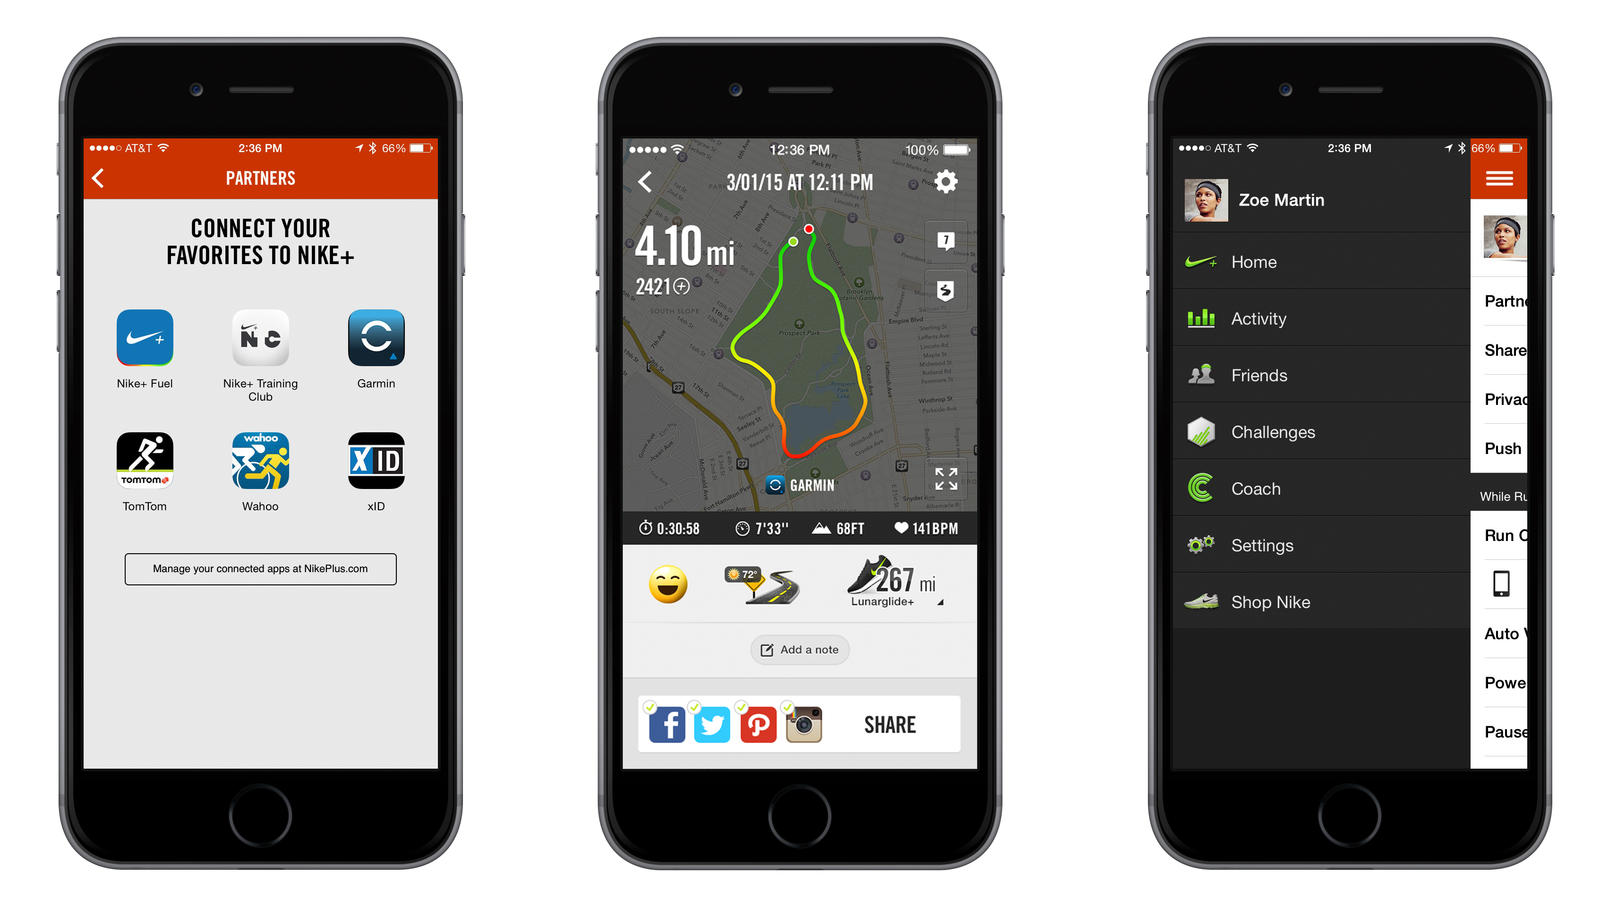
\includegraphics[width=0.5\textwidth]{nike-plus}
\caption{Nike+ mobile app. \textit{Source: http://news.nike.com/news/nike-running-expands-global-partnerships-to-motivate-more-runners-around-the-world}}
\label{nike-plus}
\end{figure}

A popular example of gamification and serious games is Nike+, which is a system that employs several game elements in order to provide a game playing experience to participants \cite{Nike} (Figure \ref{nike-plus}). Nike+ encourages players to use Nike+ equipment (e.g. Nike+ FuelBand, Nike+ shoes, or Nike+ Run Club mobile application) to keep track of and upload their exercise data (points and levels) to online leaderboards, which can be used to compete with themselves and their friends. Nike+ also keeps players motivated by playing motivational messages from their friends and elite Nike athletes (community collaboration). While Nike+ encourages players to have fun, the main goal of the game is to help players become motivated enough to improve their health through exercise. Players use these game mechanics to achieve this more serious goal. Nike+ uses 

\begin{figure}[h]
\centering
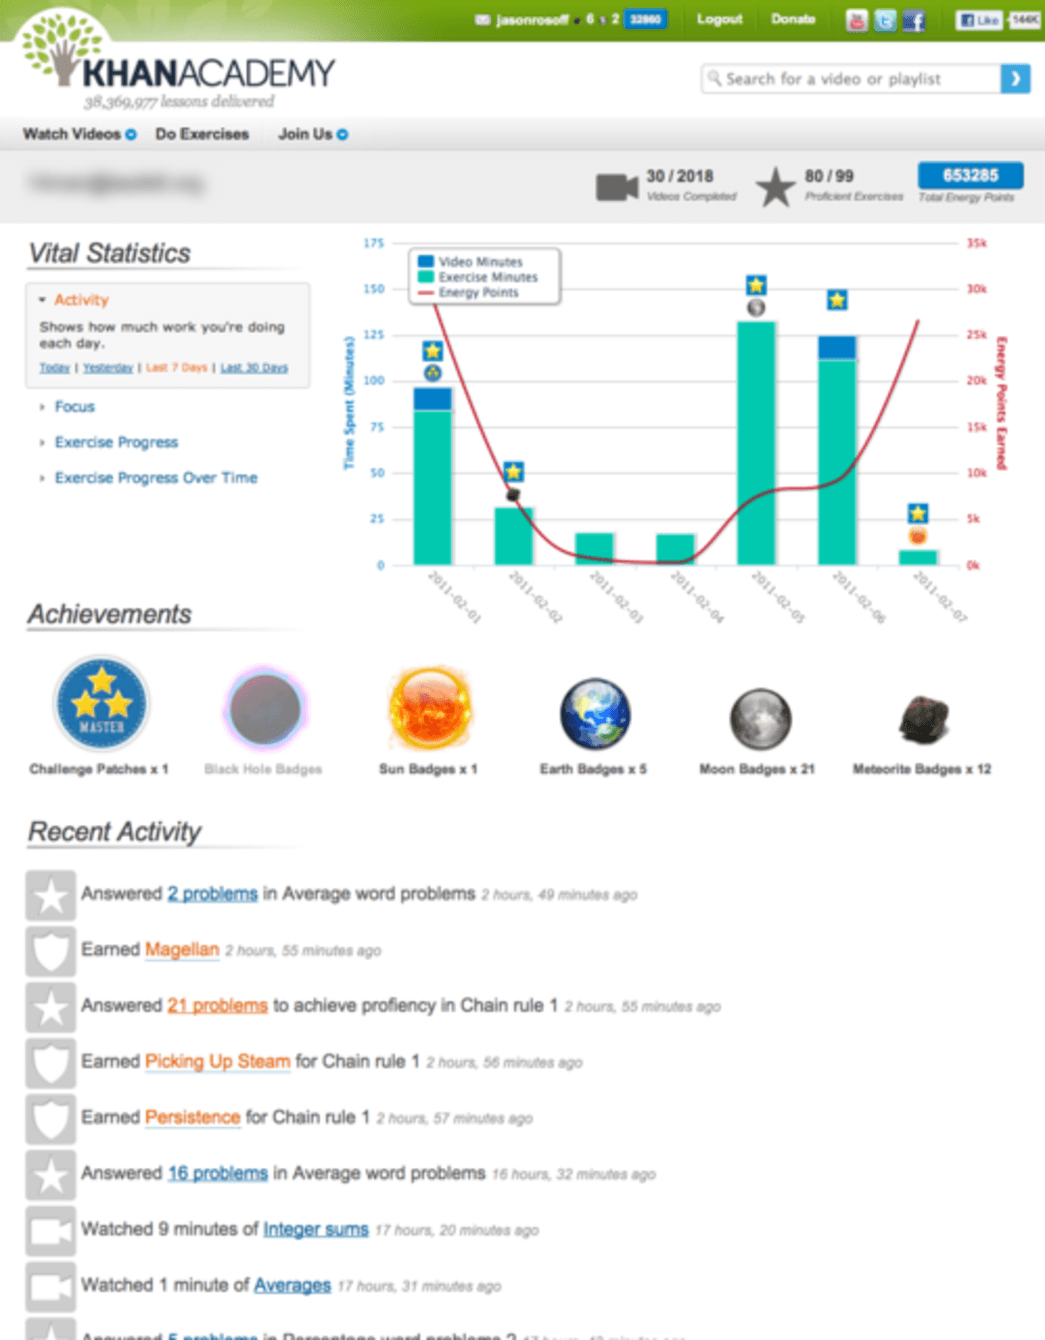
\includegraphics[width=0.5\textwidth]{khan-academy}
\caption{Khan Academy keeps track of user statistics such as badges earned and minutes spend accessing the content. \textit{Source: https://phys.org/news/2015-03-gamification-harnesses-power-games.html}}
\label{khan-academy}
\end{figure}	

Another example of gamification and serious games are gamified online courses at Khan Academy. Khan Academy teaches traditional subject matter through educational videos, and keeps users engaged through various game mechanics \cite{khan_academy}. For example, subjects are organized with skill growth trees, which show users how different skills build on top of each other. As users go through the course, they get the feeling of "leveling up" and progressive knowledge building (progression). Mundane tests are also replaced with challenges (quests), which reward players for quick problem solving and getting answer "streaks." Players will have to answer ten questions correctly to pass the challenge. If they get stuck, they have several options--they could sacrifice their streak and ask for the solution, or they could review the material with no penalty. Additionally, Khan Academy keeps track of your progress using several different statistics--how many points or badges you have earned, how many minutes you've spent watching instructional videos, and how many minutes you've spent solving problems--and displays them with attractive infographics, that help users keep track of their progress. 

\subsection{Gamification and Academic/Professional/Social Engagement}

Clearly there are certain aspects about popular video games that make them so enjoyable, addictive, and satisfying to so many people. Even the two students who initially declared that they ``don't have time for games" or simply just don't play games eventually admitted that they did play Pokemon Go at one point. Studies have shown that this human attraction to games may be caused by regular releases of dopamine that get released while playing games \cite{Koepp}. 

The four popular video games and the two serious games discussed above have a few things in common: multiplayer, small and large rewards throughout the game, additional rewards given simply for putting in time, and the persistence of the player. Many of the games also include a team aspect which encourages players to work together to advance individually. 

The multiplayer aspect of the games allows players to interact with and become competitive with other players. Rather than only beating one's own score, these games allow players to compare themselves with others and advance relative to other players, rather than simply advancing relative to their past selves. Multiplayer games encourage healthy competition, which can cause players to become more motivated.   

The format of the rewards in these games suggest that small rewards as well as large rewards throughout the game, given for a diverse amount of tasks, continues to motivate players and make sure that they do not get discouraged. These awards are often just ranks or an in-game item that can help the player to improve. 

Another similarity in the games discussed above is the rewards given to players simply for putting in time to play (e.g. EXP points, or amount of minutes put in to watching videos for Khan Academy). While players who constantly lose may feel unmotivated and lose interest, if they are given some kind of point just for trying, it makes their attempts seem less fruitless. Players should be encouraged to play, and even more so if they encounter problems. 

The persistence of the player in these video games allows players to continuously improve over time, rather than starting anew with each game. When players can see their improvements, they can be reminded of their past progress, and be encouraged to continue the progress, regardless of how grueling it may be. Once users see that they have done it before, they will know that they can do it again. 

Finally, the team aspect of many of these games suggest that many players enjoy working together with other players to achieve both team and individual goals. This shows that when people work together, they can become stronger both as a team and individually (e.g. working together to complete a mission in Overwatch, or sending motivational messages to friends in Nike+). 

\nocite {Carini}
\nocite {Junco}
\nocite {Kuh}
\nocite {Chen}
\nocite {Handelsman}
\nocite {Junco2011}
\nocite {Zhao}
\nocite {Kuh2001}
\nocite {Kuh2003}
\nocite {Huang}


\chapter{Survey Design}
\label{surveyDesign}
The experimental design of RadGrad includes three steps: a baseline assessment, a post-deployment assessment, and a final comparison between the two. These assessments will be given to current undergraduate ICS students and prospective ICS students. It will be deployed electronically via Google Forms and prospective ICS students will be given the assessment during their initial advising session. Current ICS students will be given the assessment during any voluntary advising session and also voluntarily through their ICS courses. Ideally, at least 50 responses will be gathered for both assessments.
\section{Baseline Assessment}
\label{baselineAssessment}
	The baseline assessment will contain the following questions. The full assessment can be found in Appendix A. 

\subsection{Basic Information}
\begin{enumerate}
\item \textit{What is your gender? }
Goal: Since the ICS program currently has significantly more male students than female students, what are are the differences between the experiences of the two genders? Could this give any insight into why there are so little female students? Is this something RadGrad could address? After implementing RadGrad, have there been any differences in the gender ratio or the disparity between the experiences of the two genders? Ideally, both genders should have equally positive experiences in the ICS program.
\item \textit{What is your current status in the ICS degree program?}
Goal: How do student experiences evolve as they progress through the ICS degree program? Are there any patterns? Does RadGrad have any effect on this? Ideally, students from all levels should have equally positive experiences in the ICS program. 
\end{enumerate}

\subsection{Prospective ICS Students}
\begin{enumerate}
\item\textit{ How EXCITED are you about entering the ICS program? Rank from 1-5.}
Goal: Compare this answer to the same question on the post-deployment assessment.  This will provide information regarding how students view the ICS department, based solely on outside information and before their own experiences. Ideally, RadGrad will create more excitement among prospective students due to better presentation and the appearance of a strong, supportive community and satisfied alumni.
\item \textit{How INTIMIDATED do you feel about entering the ICS program? Rank from 1-5.}
Goal: Compare this answer to the same question on the post-deployment assessment.  This will provide information regarding how students view the ICS department, based solely on outside information and before their own experiences. Ideally, RadGrad will create less intimidation among prospective students due to the appearance of a strong, supportive, and diverse community and satisfied alumni. 
\end{enumerate}

\subsection{Current ICS Students}
\begin{enumerate}
\item \textit{Which of the following extracurricular activities, if any, pertain to you? }
Goal: Compare this answer to the same question on the post-deployment assessment. Ideally, RadGrad will increase the amount of student involvement in outside ICS-related activities due to providing students with stronger connections to the ICS community.
\item \textit{Do you feel that you get enough support from others in the ICS department?}
Goal: Are students lacking support in certain areas? How can RadGrad help to address this? Compare this answer to the same question on the post-deployment assessment. Ideally, RadGrad will provide a way to give more students the support they desire from others in the department. 
\item \textit{As a student, do you feel like you have a voice to make changes within the department?}
Goal: If most students indicate that they do not feel like they have a voice within the department, what can RadGrad do to address this problem? Compare this answer to the same question on the post-deployment assessment. Ideally, RadGrad will cause more students to feel like they do have a voice to make changes in the department.
\item \textit{What makes you proud to be a part of the ICS department?}
Goal: This provides information about how current students view the department. A successful department should have a positive reputation among students, which can be manifested with a sense of pride. Compare this answer to the same question on the post-deployment assessment. Ideally, RadGrad will cause positive changes in the ICS department's reputation, leading to a greater sense of pride among students, which may play a role in students' success
\end{enumerate}

\subsection{Current ICS Students: Influences}
\begin{enumerate}
\item \textit{To what extent have ICS alumni influenced your development in the ICS program?}
Goal: Compare this answer to the same question on the post-deployment assessment. Ideally, RadGrad will facilitate more student-alumni interaction, and cause more students to be influenced in some way by an alumn in an ICS-related way.
\item \textit{To what extent have ICS peers influenced your development in the ICS program?}
Goal: Compare this answer to the same question on the post-deployment assessment. Ideally, RadGrad will facilitate more peer interaction, and cause more students to be influenced in some way by a peer in an ICS-related way.
\item \textit{To what extent have you influenced your ICS peers’ development in the ICS program?}
Goal: Compare this answer to the same question on the post-deployment assessment. Ideally, RadGrad will facilitate more peer interaction, and cause more students play a role in influencing their peers in an ICS-related way.
\end{enumerate}

\subsection{Graduating ICS Students}
\begin{enumerate}
\item \textit{Now that you are nearing the end of your ICS degree program experience, how well prepared do you feel to find a job after graduation?}
Goal: If the ICS department is fulfilling its duty, most graduating students should feel at least adequately prepared (ideally well prepared) for the future. If most students indicate that they do not feel prepared, what can RadGrad do to address this problem? Ideally, after deploying RadGrad, a higher percentage of students will feel either adequately prepared or well prepared for the future.
\item \textit{If you answered above that you feel unprepared to find a job after graduation, please explain why. }
Goal: Are there any common reasons for students not feeling prepared? If so, is there anything RadGrad can do to address this problem? Ideally, after deploying RadGrad, there will be a lower percentage of students who indicate the same problems as the preliminary questionnaire. 
\end{enumerate}

\section{Post-Deployment Assessment}
The post-deployment assessment has not yet been created, and will be created after deploying RadGrad. A section of the post-deployment assessment will contain the same questions as the preliminary assessment, with some additional choices where necessary to include RadGrad. Another section of the post-deployment assessment will contain questions specific to the student's reactions to using different aspects of RadGrad. In addition to the assessment, post-deployment analysis will include data from at least 10 interviews with RadGrad users to get more detailed information about the users' experiences.

\section{Comparison}
After all results of both assessments have been collected (ideally 50 each), they will be compared regarding student expectations versus reality, student satisfaction with the department, student engagement, and student feelings. The overall goal of RadGrad is to see suggestions of positive changes between the preliminary questionnaire and a post-deployment questionnaire that reflect less disparity between student expectations and reality, greater student satisfaction with the department, more student engagement, and more positive student feelings. These changes will support the hypothesis that RadGrad could cause several significant and positive changes with the students of the ICS department.
\chapter{System Design}
I believe that the best way to address current ICS student issues is through an online system that combines degree planning, social networking, and gamification. The specific features of the system evolved over time through a process conducted in Fall 2015-Spring 2016 by Philip Johnson. This process incorporated feedback from the four major RadGrad user groups: students, faculty, academic program advisers, and alumni/local high tech community members. Spring 2015 students in Software Engineering II became directly involved in the design process by creating their own paper and HTML mockups and by doing user tests and analyses on their suggested systems. Faculty members and academic program advisers provided feedback through a RadGrad advisory board and through advising sessions. Alumni and local high tech community members became involved through RadGrad talks at local tech meetups. In this chapter, I present the design of the RadGrad system resulting from these activities. 
\section{Degree Planner}
\subsection{Degree Plan}
Each student in RadGrad will have a degree plan, which displays the student's courses, extracurricular activities, and outside work on a semester-by-semester basis. This plan contains future data as well as historical data. This allows students to easily view their progress and prepare for the future. 
\subsection{Degree Goal}
Although each student is aiming for a bachelor's degree in ICS, a more specific goal is beneficial in helping the student find a focus for their education and career goals. Some of these specific goals include B.S./B.A/B.S Computer Engineering and Security/Ph.D. Prep/Silicon Valley Tech. By specifying these specific goals in a concrete way, students can feel less overwhelmed by the large expanse of ICS classes, more prepared for the future, and more easily form communities of interest with other like-minded students.
\subsection{Dashboard}
Each user has access to a personal dashboard, available upon login. This dashboard provides a quick look at some of the user's stats, such as current ICS GPA, current ICS credits awarded, summary of schedule, current degree goals, interest tags, user picture, suggested vignettes, stoplight, recommendations, currently active petitions, and predictions. This is a quick and easy way to provide students with a variety of information on their overall progress in their major. 

\subsection{Recommendations}
Recommendations aim to help students understand how to change their current behavior to improve their ICS experience. Unlike Starfish by Hobsons, RadGrad will base recommendations on a factors beyond academics, such as the student's current degree plan, degree goals, and professional interests. Some examples of possible recommendations are: relevant courses or extracurricular activities not already present in their degree plan, an estimate of ideal maximum work hours, predicted impact of their GPA, and relevant mentorship opportunities that are not being taken advantage of. 
\subsection{STAR Interface}
RadGrad will request a relationship with the UHM STAR website, which will provide students with their current and past courses and their resulting grades. This will allow students to see all of their relevant course information in the same place that they get all their other ICS information. RadGrad could also integrate with the STAR scholarship database to find ICS-related scholarships and encourage students to apply for them, based off their information and goals. For instance, if one of the student's main goals is to graduate debt-free, they should be informed of applicable scholarships. In addition to the information provided by STAR, since the database will be much smaller, RadGrad could provide more specific details about each scholarship, how to become eligible, and how to apply. 
\subsection{Workload Adviser}
RadGrad will implement a virtual workload adviser, which will combine the student's course load, outside work hours, ICS grade data, and employer expectations to give the student advice on how much work they should be taking on at one time. It will offer suggestions, such as ``If you drop 1 ICS course and reduce your work hours to 10 per week, the average ICS GPA is 3.4." Unlike Blackboard Planner, RadGrad offers suggestions for students in the present time, rather than just for the future. This can help students to have a more realistic view of their goals, prevent students from getting burnt out, reduce stress levels, and encourage a healthier school-work balance.

\section{Degree Planner: Possible Further Implementations}
\subsection{Predictions}
Each student will have a prediction model, which predicts post-graduation aspects based upon recent graduates, data from local tech organizations, recruiters, headhunters, etc., and data from the ICS faculty. This data is then combined with the student's individual degree plan and degree goals to produce a customized prediction.  This feature will hopefully help students feel better prepared for their future after graduation.

\section{Social Network}
\subsection{Profile}
Students, faculty, graduates, and administrators will each have their own respective profiles. Student profiles will contain personal information including name, email, details about their degree, images, interests, projected graduation date, and professional recommendations based off their inputted information. Faculty profiles include name, email, image, professional interests, and descriptions of current projects they are working on. Graduate profiles will include details about their life after graduation such as place of employment and position description. All profiles will be publicly available so that the ICS community can view each others' profiles and find connections. 

On a gamification level, profiles also allow users to be persistent and easily view their progress. Since each user has a username and profile, they will be persistent on RadGrad, and all of their achievements will build up on their profile as they progress through college and beyond.
\subsection{Course Feedback}
As a supplement to the UH system's end-of-semester course feedback system, RadGrad offers a mid-semester public course evaluation system. This allows students to reach out and communicate with each other and professors to make the learning experience as ideal as possible for all parties, while there is still time left in the semester. Ideally this will improve the quality of courses, the satisfaction of the students, and the teaching abilities of the professors. Unlike Rate My Professor, this process is not anonymous, and encourages professors to improve, rather than encouraging other students to avoid a certain course. 
\subsection{Degree Feedback}
RadGrad will reach out to ICS alumni approximately six months after graduation. At this time, these ICS graduates will answer a number of questions regarding their life after graduation (i.e. graduate education, career prospects, retrospective thoughts about the ICS department, etc.). This feature will provide data that will help the ICS department improve their degree program, and also provide clear and convenient lines of communication between alumni and the ICS department. 
\subsection{Feedback and User Evaluation}
RadGrad will provide a easy and convenient way for users to provide RadGrad feedback about the system. There will be links for immediate feedback, and there will also be yearly surveys to measure user satisfaction over time. By providing an easy stream of communication between users and RadGrad developers, RadGrad can be constantly growing along with the department in order to serve their evolving needs as best as possible.

\section{Social Network: Possible Further Implementations}
\subsection{Department Feedback}
Any type of user can initiate department feedback by starting a petition. The petition will be public, and any other user can edit it as well. Once the editors of the petition reach a consensus and get at least 20 votes of confidence from other users, the user will become finalized and other users may sign the petition over a course of two weeks. The petition will then be discussed at a faculty meeting, eventually leading to the petition being implemented, not implemented, or deferred. By giving users a platform to easily collaborate with each other over a common cause, members of the ICS department will feel more empowered, more involved, and ideally more satisfied.

\subsection{Mentorship}
RadGrad users can be certified mentors if they are in ICS 390 or a TA. A student is working under a mentor if they are a ICS 499 student working under a professor or participating in a research group opportunity under a faculty sponsor. There can be other possible instances of mentorship, and over time, a network of mentorships will form, which could possibly help foster more and better mentorships with future students.

\subsection{Billboard}
RadGrad can also provide some physical hardware (i.e. a large monitor) to be displayed in the ICS department. This display will show aspects of RadGrad (i.e. statistics gathered from RadGrad, upcoming events, current petitions, etc.). This will further encourage engagement throughout the department, as it will be a constant reminder of the current status of the community, and will perhaps contribute to promoting an overall closer ``community" feel. 

\section{Gamification}
\subsection{Stoplight}
The stoplight is a UI widget embedded in the dashboard, which takes on the appearance of a traffic stoplight, and uses the red/yellow/green colors to indicate the extent of that student's ICS activity. The light is green if the student is taking excellent advantage of what the department has to offer. The light is yellow if the student is taking sufficient advantage of what the department has to offer, and the light is red if the student is not taking enough advantage of what the department has to offer. To determine this, the stoplight takes into account the student's professional interests and goals, their GPA, available opportunities, the opportunities they have taken advantage of, the available courses, and the courses that the student has taken. By being encouraged by the changing colors of this stoplight, fueled solely by the student's actions, students may take this as a personal challenge, or game, to keep the stoplight at a certain color as much as possible. This is a simple way for students to track their progress throughout their ICS journey. This is an example of small rewards that are given throughout the "game" of ICS--students can visually see improvement, as though they are achieving a new rank. Similarly to EXP points in games, students can get these achievements simply by putting in more time and effort. They don't necessarily have to win a Hackathon or get straight A's, but as long as they are participating and putting in the effort, it will show on their Stoplight. 

\subsection{Leaderboard}
A public leaderboard will be available for students to actively compare themselves against others in the department in terms of ICS GPA, velocity (a calculated value indicating a student's progress through the program), and professional preparation (a calculated value combining coursework and extracurricular activities). An award ceremony type of tradition could be started out of this, which awards high ranking students. This type of active and constant comparison could help foster healthy competition and higher engagement among students. This is an example of the multiplayer aspect of the aforementioned games that foster healthy competition and drive within players. Without the RadGrad network, students are left mostly oblivious to the progression of others and only have themselves to relate their progress to. If a student has always progressed slowly, that student may believe that he/she is continuing to do well, as long as they do not begin to progress even slower. With RadGrad, this student would be able to see the quicker progression of other students, and suddenly create a different goal in his/her mind.

\subsection{Gamification: Possible Further Implementations}

\subsection{ICE}
ICE is an acronym for Innovation (i.e. a student's involvement in research or other innovative activity), Competency (i.e. a student's grades in ICS courses), and Experience (i.e. a student's involvement in high tech environments through internships or other professional activities). ICE is a measurement of these aspects, calculated using the information provided on the student's profile. This balances the three aspects to emphasize the importance of all three in an ideal ICS experience. Details on how these aspects are measured can be found at www.radgrad.org. These clear measurements of ``success" can be eye opening for students. It can be easy to get caught up in the minor details of a major and lose track of the bigger picture. ICE helps students to remind themselves to balance their ICS experiences out, in order to become as attractive as possible for future employers. This feature can also be physically manifested in terms of badges or stickers, as a symbol of rank. This can encourage students to become more competitive and therefore less lazy and more productive. (It helps that a lot of ICS students enjoy the incentives provided by video games.) This is also an example of the rewards and competitive multiplayer aspect of many popular video games. 





\chapter{Survey Results}
\label{survey-results}
Coming soon!
\chapter{System Results}
\label{system-results}

\section{Development}
\subsection{Frameworks and Environments}
RadGrad was built using the Meteor JavaScript web framework. Meteor is integrated with MongoDB and uses the Distributed Data Protocol and publish-subscribe pattern to create real time, responsive code that automatically updates data changes to the client. On the client side, RadGrad uses jQuery and Semantic UI to design and create the user interface. Due to excellent Meteor integration, RadGrad was developed using IntelliJ IDEA. In an effort to create clean and uniform code, RadGrad uses ESLint to confrom to the AirBnB Javascript Style Guide. 

\subsection{Project Management}
We developed RadGrad using GitHub issues and GitHub projects. Development tasks are created as a GitHub issue, and each issue has an assigned developer and and assigned branch. Each issue also resides in a GitHub project, which groups issues together to mark larger milestones. When the developer begins actively working on the issue, they will move the issue in the milestone from a ``Backlog" column to an ``In Progress" column. Once the developer completes the task in the specified branch, they will close the issue and move the issues in the milestone from the ``In Progress" column to the ``Done" column. The RadGrad developers typically communicate through Slack and in person meetings twice a week. 

\section{Data Model}
\subsection{Career Goals}
Career goals represent possible ICS related careers that ICS students can aspire to get after graduation. Each career goal has an associated name, slug, description, related interests, and an optional URL for more information. Students can choose as many career goals as they want. Faculty and mentors can choose career goals that they would like to be associated with as well.  

\begin{table}[h!]
\centering
\begin{tabular}{ l l l } 
 Data Scientist & Database Administrator & DevOps Engineer \\ 
 Full Stack Developer & Game Developer & Graduate School \\ 
 Information Security Analyst & Information System Manager & IoT Architect \\ 
 Mobile App Developer & Network Engineer & Research Scientist \\
 Robotics Engineer & Software Developer & Startup Co-Founder \\
 Teacher & UX Designer & VR/AR Engineer 
\end{tabular}
\caption{List of RadGrad career goals as of April 2017}
\label{table:1}
\end{table}

\subsection{Courses}
Courses represent all past, present, and future ICS courses. Each course has an associated name, short name, slug, course number, description, credit hours, related interests, a syllabus URL, a URL for more information, and associated prerequisites. The course name is the official name appearing in the UH registration guide, and the course short name is used for display purposes. Students may add as many courses as they would like to their degree plan. 

Course instances represent individual instances for each student. Each course instance has an associated semester, course, whether it has been verified or not, whether it came from STAR or not, grade, credit hours, note, student, and associated ICE points. A course instance is considered verified if ???. A course instance has a note if it is not an ICS course. It is important to note that course instances on RadGrad are only valid on RadGrad, and students must use other methods to officially make UH course registration changes.

\subsection{Desired Degrees}
Desired degrees represent all past, present, and future ICS degrees. Each desired degree has an associated name, short name, slug, and description. Students can only choose one desired degree at any given time. However, they are free to switch desired degrees as many times as they want. It is important to note that desired degrees on RadGrad are only valid on RadGrad, and students must use other methods to officially change their declared degree at UH. 

\subsection{Degree Plan}
Degrees plans represent all past, present, and future ICS degree plans. Each degree plan has an associated degree, name, effective semester, amount of courses per semester, and list of courses. Students can view degree plans if they would like a more specific focus than just a broad BS or BA degree. Examples of degree plans are ``BS in Computer Sciences Security Sciences", ``BA in ICS Security Science Focus", and ``BA in Computer Sciences IT Focus." Students can look at any plan at any time to see what they would need to do to fulfill it. It is important to note that these degree plans change over time, and a ``BS in Computer Sciences Security Sciences" may be different in 2016 than in 2018. This is why both year and plan name must be chosen when selecting a plan.  

\subsection{Feeds}
Feeds represent select actions of RadGrad users. Each feed has associated users, opportunity, course, semester, description, time stamp of the action, picture, and feed type. A feed could have one or multiple users. There are currently six different feed types: a new RadGrad user is added, a new course is added to RadGrad, a new opportunity is added to RadGrad, a user has been verified for completing an opportunity, a new course review has been added, and a new opportunity review has been added. These particular actions have been selected because they could be useful and of interest to other RadGrad users.

\subsection{Feedbacks}
Feedbacks represent recommendations and warnings for students. Each feedback has an associated name, slug, description, and feedback type. There are currently two feedback types: recommendation and warning. 

Feedback instances represent individual instances for each student. Each feedback instance has an associated feedback, user, description, and area. There are currently four different areas: interests, ICE, STAR, and degree plan. Each time the student's plan changes, feedback instances in these areas are deleted and recalculated.

\subsection{Help Messages}
Help messages represent guidance for a particular RadGrad page. Each help message has an associated route name, title, and text. The text can contain actual text, images, and formatting. Each page (route name) can have at most one help message. These help messages are displayed at the top of the specified page, in a collapsible pane.  

\subsection{ICE}
ICE represents a student's ICE points. Each ICE has an associated number for ``I", ``C", and ``E." There are two types of ICE points: earned and planned. Earned ``I" and ``E" points are calculated by adding the ``I" or ``E" points for each verified opportunity in the student's plan. Earned ``C" points are calculated by adding the ``C" points for each verified course in the student's plan. The amount of earned points for each course depends on the grade that the student received; A's represent more points than B's. Planned ``I" and ``E" points are calculated by adding the ``I" or ``E" points for each unverified opportunity in the student's plan. Planned ``C" points are calculated by adding the ``C" points for each unverified course in the student's plan. A student's earned and planned ICE points are updated each time there are changes to the student's degree plan. 

\subsection{Interests}
Interests represent possible ICS related interests that RadGrad users could have. Each interest has an associated name, slug, description, interest type, and a URL for more information. All RadGrad users may choose to be associated with as many interests as they would like. 

\begin{table}[h!]
\centering
\begin{tabular}{ l l l } 
.NET & Algorithms & Android \\ 
Application Development & Artificial Intelligence & Assembler \\
Bioinformatics & Biology & C and C++ \\
C\# & Civic Engagement & Cognitive Science \\
Computer Architecture & Computer Ethics & Computer Graphics \\
Computer Vision & Cryptography & Data Science \\
Data Visualization & Databases & Entrepreneurship \\
Game Design & Graphic Design & Hardware \\
High Performance Computing & Human-Computer Interaction & IT Management \\
Java & Javascript & LInux \\
Lisp & Machine Learning & Mobile Computing \\
Networks & Operating Systems & Parallel Programming \\
Perl & Prolog & Psychology \\
Python & R & Research \\
Robotics & Ruby & Software Development \\
SQL & Security & Sustainability \\
Teaching & Theory of Computation & Unity \\
Virtual Reality & Web Development & iOS
\end{tabular}
\caption{List of RadGrad interests as of April 2017}
\label{table:2}
\end{table}

\subsection{Levels}
Levels represent a student's RadGrad level. There are six possible levels, from Level 1 to Level 6. A student's level is calculated based off the amount of ICS courses they have passed, the amount of opportunities they have done, and the amount of reviews they have contributed on RadGrad. Levels are calculated each time ??? 

\subsection{Advisor Logs}
Advisor logs represent an interaction between an ICS advisor and a student. Each advisor log has an associated student, advisor, text, and date created. A new log can be created by the advisor whenever they have a meeting with a student. Advisors and students can use these logs to keep track of when meetings were held, and what occurred at these meetings. 

\subsection{Mentors}
The mentor data model includes three parts: mentor profiles, mentor questions, and mentor answers. Each mentor profile has an associated mentor, company, career, location, LinkedIn, and a message about what motivated them to become a mentor. Each mentor will have exactly one mentor profile.  

Each mentor question has an associated title, slug, student, whether it is moderated or not, whether it is visible or not, and moderator comments. Students can create as many mentor questions as they would like. However, each question needs to be approved by moderation in order to be visible to the public. Advisors and administrators have the ability to moderate questions. If a question is declined by moderation, the moderator can add reasons for the decline in the moderator comments field. The student can then see the feedback, and they are able to either edit their question and send it back to moderation, or simply discard the question. There is no limit to how long the back and forth process between student and moderator can go on. 

Each mentor answer has an associated question, mentor, and text. Each mentor question can have any amount of mentor answers, but each mentor answer can answer at most one mentor question. Each mentor question can only be associated with exactly one mentor. There is no moderation process for mentor answers, and submitted mentor answers are automatically visible on RadGrad. 

\subsection{Opportunities}
Opportunities represent all past, present, and future ICS related opportunities.  Each opportunity has an associated name, slug, description, opportunity type, sponsor, related interests, icon URL, semesters available, event date, whether it is an independent study or not, URL for more information, and ICE points. Currently, there are five opportunity types: club, event, internship, online learning, and project. The opportunity sponsor is any faculty member who is the point of contact for the opportunity. If the opportunity occurs on a semester basis, it will have associated semesters. If the opportunity occurs on a specific date, it will have an associated event date. The amount of ICE points varies depending on the nature of the opportunity, and is determined by RadGrad administrators. 

Opportunity instances represent individual instances for each student. Each opportunity instance has an associated semester, opportunity, whether it is verified or not, student, and ICE points. An opportunity instance can only be verified by a RadGrad advisor or faculty. Two students that each have an opportunity instance for the same opportunity could have different ICE points depending on the extent of their involvement in the opportunity.    

\subsection{Public Stats}
Public stats calculate 24 different RadGrad statistics from the current database. The statistics calculated are: total courses, total career goals, list of career goals, total desired degrees, list of desired degrees, total interests, list of interests, total opportunities, total project opportunities, list of project opportunities, total users, total students, total faculty, total mentors, list of mentor professions, list of mentor locations, total course reviews, list of courses reviewed, total level one students, total level two students, total level three students, total level four students, total level five students, and total level six students. Public stats are automatically recalculated once each day at midnight. 

\subsection{Reviews}
Reviews represent all course and opportunity reviews written by students on RadGrad. Each review has an associated slug, student, review type, reviewee, semester, rating (Figure 6.1), comments, whether it is moderated or not, whether it is visible or not, and moderator comments. There are two review types: course and opportunity. The reviewee refers to the course or opportunity that is being reviewed. Each review must have a rating from one to five stars. Each student may review a course once the semester they have taken it in has passed. Each student may review an opportunity once the opportunity has been verified. Each student can review each course or opportunity at most once. Each review is visible to the public by default, but can be removed by moderators. Advisors and administrators have the ability to moderate reviews. If a review is declined by moderation, the moderator can add reasons for the decline in the moderator comments field. The student can then see the feedback, and they are able to either edit their review and send it back to moderation, or simply discard the review. There is no limit to how long the back and forth process between student and moderator can go on. A student can also update their review at any time, but this will mean that the review will go through the moderation process again.

\begin{figure}[h]
\centering
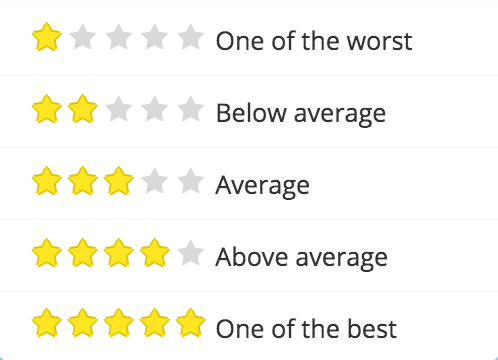
\includegraphics[width=0.5\textwidth]{datamodel-reviews}
\caption{Course and opportunity review ratings.}
\end{figure}

\subsection{Roles}
Roles represent the different user roles allowed in RadGrad. There are currently six roles: faculty, student, admin, alumni, advisor, and mentor. Currently, users are allowed to have exactly one role. All users except for admin and advisor can view only their own RadGrad pages. Advisors can also view student RadGrad pages, and admin can view all RadGrad pages. 

\subsection{Semesters}
Semesters represent an academic semester at the University of Hawaii. Each semester has an associated term, year, number to sort by, semester number, and slug. There are three possible terms: Spring, Summer, and Fall. The number to sort by easily allows chronological comparisons between semesters. Semester number is used for ??? 

\subsection{Slugs}
Slugs are strings used as part of a URL to uniquely identify an entity. These strings do not change with different instantiations of the database like docIDs do. Slugs are used in the RadGrad data model to represent relationships between different entities. Therefore, only collections that need to be referenced by other collections contain a slug. 

\subsection{Teasers}
Teasers represent short videos that advertise an ICS opportunity. Each teaser has an associated title, slug, author, URL, description, duration, related interests, and opportunity. Any member of RadGrad can be an author of a teaser. Teasers are typically less than a minute long and function as a sort of quick advertisement to get potential students interested in participating in that particular opportunity. 

\subsection{Users}
Users represent anyone who has created an account on the RadGrad system. Each user has an associated username, first name, last name, slug, email, password, UH ID, career goals, interests, desired degree, picture, level, website, hidden courses, and hidden opportunities. The user's RadGrad username is the same as their UH email name. This, along with their email, cannot be changed once the user's account is created. Only student users will have a desired degree and a level. Hidden courses and hidden opportunities are used to keep track of courses and opportunities that students have actively ``hidden" from their page. By keeping track of these hidden courses and opportunities, students can have the option to make them visible again.

\subsection{Verification Requests}
Verification requests represent a request from a student to get verification and ICE points for completing an opportunity. Each opportunity has an associated date, status, verifier, and feedback. There are three possible statuses: accepted, rejected, and open. The verifier is the user who has verified the event. Only advisors, faculty, and admin can be a verifier. If a request is rejected, the verifier can add reasons for the rejection in the feedback field. The student can then see the feedback and the results of the verification. If the verifier wishes to reopen the verification request, they may do so at any time. A student who would like to reopen a request will need to contact the verifier.  

\subsection{Academic Years}
Academic years represent an academic year at the University of Hawaii. Each academic year has an associated year, spring year, student, and semesters. Since academic years start in the Fall and end in the Summer, they span two years: year, and spring year. A student on RadGrad must have an academic year for each year, or portion of a year, that they are enrolled in an ICS course or participated in an ICS opportunity.

\section{Testing}
\subsection{Interactive Testing}
RadGrad uses interactive server-side testing with Mocha test runner and Chai Expect Assertions during code production in order to maintain correctness. Each collection class from the data model has tests in a corresponding testing file. These tests include checking if a new collection entity can be defined, if a collection entity can be removed, if a collection entity can be dumped from the database, and if a collection entity can be restored from a dump file to the database. If the collection class includes additional functions specific to that collection, the test file includes tests for those functions as well.

\subsection{Personas}
In order to ensure that a wide variety of students will be able to use RadGrad effectively, we created five personas, where each persona is represented with a student user account on RadGrad. Each persona represents a student at a different part of the degree program. Below are brief descriptions of each persona. 

\begin{enumerate}
  \item Ella Zwick: Ella is a Freshman who has just declared her BA ICS major. She has not taken any ICS courses yet, and she does not have a RadGrad degree plan yet either. She is at Level 1. Her career goal is to be a web developer, and her interests are in civic engagement and web development. 
  \item Charley Sherry: Charley is a Freshman who is in his second semester of the BS CS curriculum. He is currently enrolled in ICS211 and ICS241. He is at Level 2. His career goal is to be a data scientist, and his interest is in bioinformatics.  He has at least 12 competency points for completing ICS111 and ICS141 during the previous semester. 
  \item Betty Keanu: Betty is a Junior who has completed the BS CS core curriculum (ICS111, ICS141, ICS211, ICS241, ICS311, ICS314) and is currently taking 300+ courses to fulfill the rest of her degree plan. She is at Level 4. Her career goals are graduate school and data scientist, and her interests are big data, visualization, and research. She has completed a few opportunities, and has at least 30 innovation points, at least 36 competency points, and at least 30 experience points. 
  \item Abigail Kealoha: Abigail is a Junior who is two semesters away from graduating with her BS in CS. She is Level 5. Her career goal is to be a web developer, and her interests are security and software engineering. She has completed several opportunities, and has at least 80 innovation points, at least 80 competency points, and at least 80 experience points. Abigail has also contributed one course review on RadGrad. 
  \item Alfred Persona: Alfred is a Senior in his last semester of the BS CS curriculum. He is at Level 6. His career goal is a software developer and his interests are in game design, hardware, and virtual reality. He has completed many opportunities, and has at least 100 points for each of the ICE categories. Alfred also contributed 6 course reviews on RadGrad.
\end{enumerate} 

\subsection{Beta Testing}
In Spring 2017, after completion of the major Student, Advisor, and Administrator components and pages, we held RadGrad beta tests, which invited selected students and an advisor to view and use the system for the first time. The main goals of these tests were to identify user problems, identify common aspects users like, assess if parts of the user interface are more intuitive or more difficult to use, if there are missing features that should be implemented, if certain features could be improved, and to get a feel of whether users feel that the would use RadGrad and that it would improve their engagement in the ICS degree program. We hoped this data would help us decide if the system so far is going in a promising direction.

\subsubsection{Student Beta Testing}
Student subjects were solicited over email, and were selected in a way that provided us with a wide range of student levels. Each student was given \$20 as compensation for 30 minutes of their time. Prior to the testing session, each subject provided their name and UH account, completed ICS courses, completed opportunities, interests, and career goals. Using this information, the student's RadGrad account was set up prior to the session. Each session involved one student and two RadGrad developers (an evaluator to lead the session, and an observer). At the start of the session, the evaulator briefly went over the basic ideas of the system and the different parts that they can interact with. During the second part of the session, the student was allowed to peruse the system and explore or comment on anything they found particularly interesting. During the third part of the session, the evaluator asked the student to describe what they liked about the system, what they disliked about the system, and whether or not they think they would use this system if it were available to them. See Table 6.3.

\begin{table}[h!]
\centering
\begin{tabular}{ |p{8cm}|p{8cm}|}
 \hline
\textbf{Positive Feedback} & \textbf{Problems with System} \\
 \hline
 Recommended opportunities are useful because otherwise students are only notified by Gerald's emails  & ICE points display was confusing \\
 \hline
 Reduces the amount of work currently needed for students who try to find ways to succeed beyond the classroom. &List of opportunities was hard to view because it was partially off the screen\\
 \hline
 Degree planner helpful for visualizing pathway &Annoying to have to scroll to see all possible review ratings\\
  \hline
Likes the levels and ICE gamification &Confusing to find some things without some kind of tutorial \\
 \hline
Level stickers can help students see who they might want to talk to &Performance issue with page loading times \\
 \hline
RadGrad and ICE are good at stressing the importance of activities outside of courses &Wish there were notifications for when new opportunities come up\\
 \hline
RadGrad provides extra details about courses and opportunities that were previously unknown to the student &Recommended Courses and Recommended Opportunity widgets on the student home page have non-intuitive scrolling behavior\\
 \hline
RadGrad helps degree plan to feel less ``random" &Wish there were notifications for when new opportunities come up\\
 \hline
Likes how RadGrad helps students understand the benefits of internships, which they learned too late would be helpful &Students should be allowed to opt out of showing their current and future courses and opportunities\\
 \hline
RadGrad is a good way to keep track of a degree plan, which a student previously wrote on a paper and misplaced it & Wish there were notifications for when new opportunities come up \\
 \hline
 STAR does not work adequately for many students, and RadGrad could be a good supplement for that & Wish there was less unnecessary clicking while altering the degree planner\\
 \hline
Student easily navigated degree planner UI with only some guidance &Wish there were support for specific focus areas\\
 \hline
Mentorspace could help students to get an idea of what they can actually do with their degree after graduation &Would like to know ahead of time when certain courses are being offered\\
 \hline
The fact that RadGrad helps you plan even if you have no idea what you want to do, whereas with STAR, you have to know what you want to do beforehand & Manual edits to one student's generated plan caused empty extraneous years in the degree planner\\
 \hline
Rating courses seems helpful in planning & One student's STAR data included a long gap between years, which wasn't handled well in the degree planner without manual intervention\\
 \hline
Liked how degree plan could be generated rather than manual &\\
 \hline
Liked the idea of an individual ICS online space &\\
 \hline
\end{tabular}
\caption{Student beta test results}
\label{table:3}
\end{table}

\subsubsection{Advisor Beta Test}
It was easier to solicit an advisor for the beta test, since Gerald Lau is currently the only ICS advisor. During his session, the evaluator briefly went over the system from the point of view of both students and the advisor. While Gerald did not actually get to interact with the system himself, he was able to see how it would be used, and he was able to give feedback about his perceived usefulness of the system. Gerald's response was positive overall, and he seemed interested in integrating it into future advising.
\section{Student Mode}
\subsection{Degree Planner}
\subsubsection{Degree Planner}
The student degree planner is the main place that students will go to view and make changes to their entire degree plan. Students can view up to four academic years at a time, but they can view additional past or future years by clicking on the green arrows at the bottom. Semesters that are in the past are greyed out and cannot be changed by the student. Any present or future semesters can be changed by dragging and dropping courses or opportunities into that semester pane. The grades for a course can be changed with the drop down menus. This page also includes an inspector pane on the top right hand corner, which the student can use to view brief details about a course or opportunity while planning their degree. The in-depth course and opportunity explorer pages can be accessed through the inspector, but the short descriptions in the inspector allows for quick and convenient assistance within the same view as the degree planner itself. The student can choose a course or opportunity to inspect by either choosing from the green dropdown menu at the top of the inspector, or by clicking on the course or opportunity name within the plan. 

Below the inspector is the academic plan pane. In this pane, students can select a year and an academic plan name (i.e. B.S. in Computer Science Security Science) to indicate the degree plan that the would like to follow. The pane then displays the required courses for this plan, organized into the recommended semesters, and color coded (green for classes in the student's plan, and red for classes not in the student's plan). Students can use this display to easily drag their missing courses onto their plan.

\begin{figure}[h]
\centering
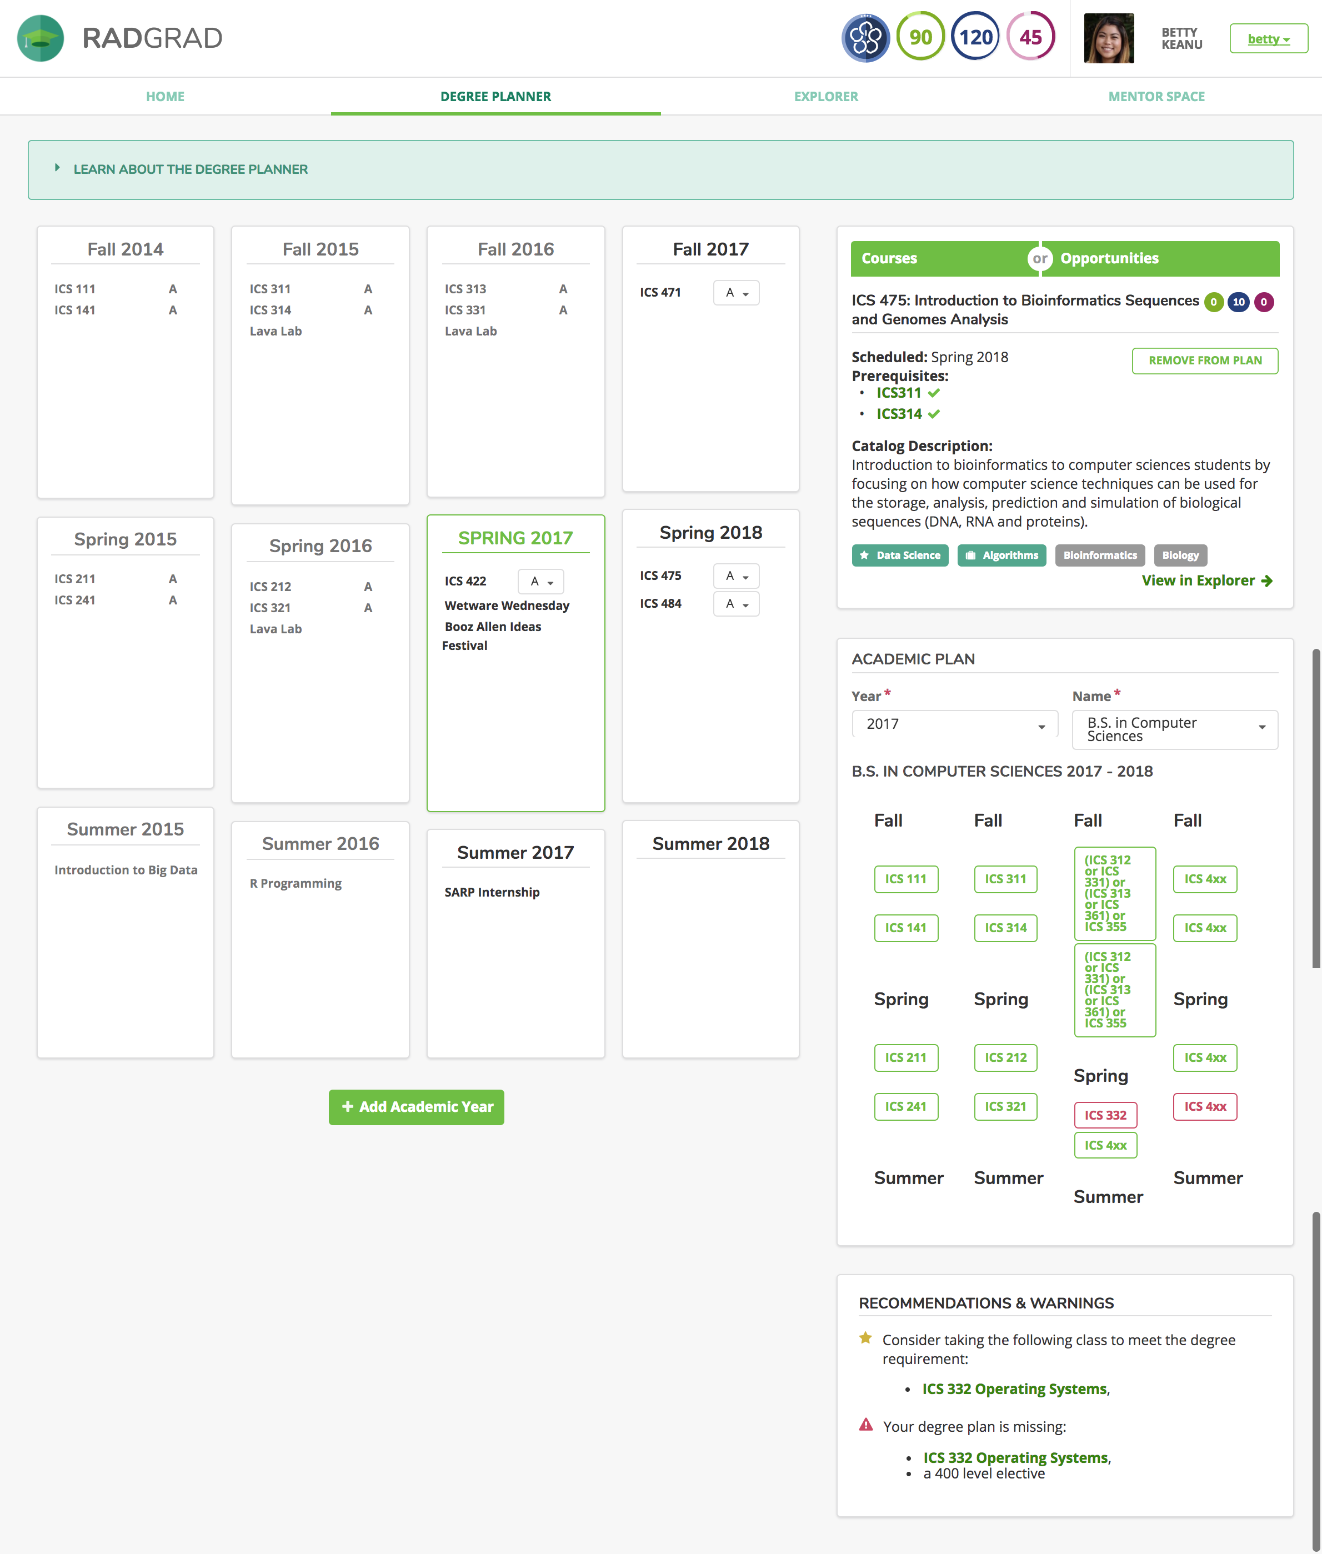
\includegraphics[width=1.0\textwidth]{degree-planner}
\caption{Degree Planner page.}
\end{figure}

\subsubsection{Recommendations and Warnings}
The student degree planner automatically generates warnings and recommendations on the bottom right hand corner. These warnings and recommendations change as a student's degree plan changes. Each time a student adds, moves, or removes a course or opportunity through the degree planner, explorer, or student home page, the warnings and recommendations will regenerate. 

On the student home page, students can see details about recommended courses and opportunities as soon as they log in. These are chosen based off the student's chosen interests and career goal related interests. If a student is interested in a particular course or opportunity, they can choose to view more in the explorer, add it to their plan, or leave it there to decide what to do with later. If a student knows they are not interested in a certain course or opportunity, they can choose to hide it by clicking the "hide" button. If the student later changes their mind, they can view and unhide the course or opportunity by clicking ``Hidden Opportunities."

\begin{table}[h!]
\centering
\begin{tabular}{  |p{8cm}|p{8cm}| } 
  \hline
 \textbf{Warnings} & \textbf{Recommendations} \\ 
  \hline
A prerequisite course is missing & Course recommended based upon interests\\
\hline
Semester appears overloaded (more than 3 ICS courses) & Opportunity recommended based upon interests\\
\hline
A required course is missing & Recommendation for ICS innovation points \\
\hline
Course is not offered in chosen semester (future implementation) & Recommendation for ICS competency points \\
\hline
& Recommendation for ICS experience points\\
\hline
& Move towards achieving the next level \\
\hline
& See your ICS advisor to upload STAR data\\
 \hline
\end{tabular}
\caption{Automatically generated warnings and recommendations as of May 2017}
\label{table:4}
\end{table}

\subsubsection{Career Goal, Course, Desired Degree and Opportunity Explorers}
\begin{figure}[h]
\centering
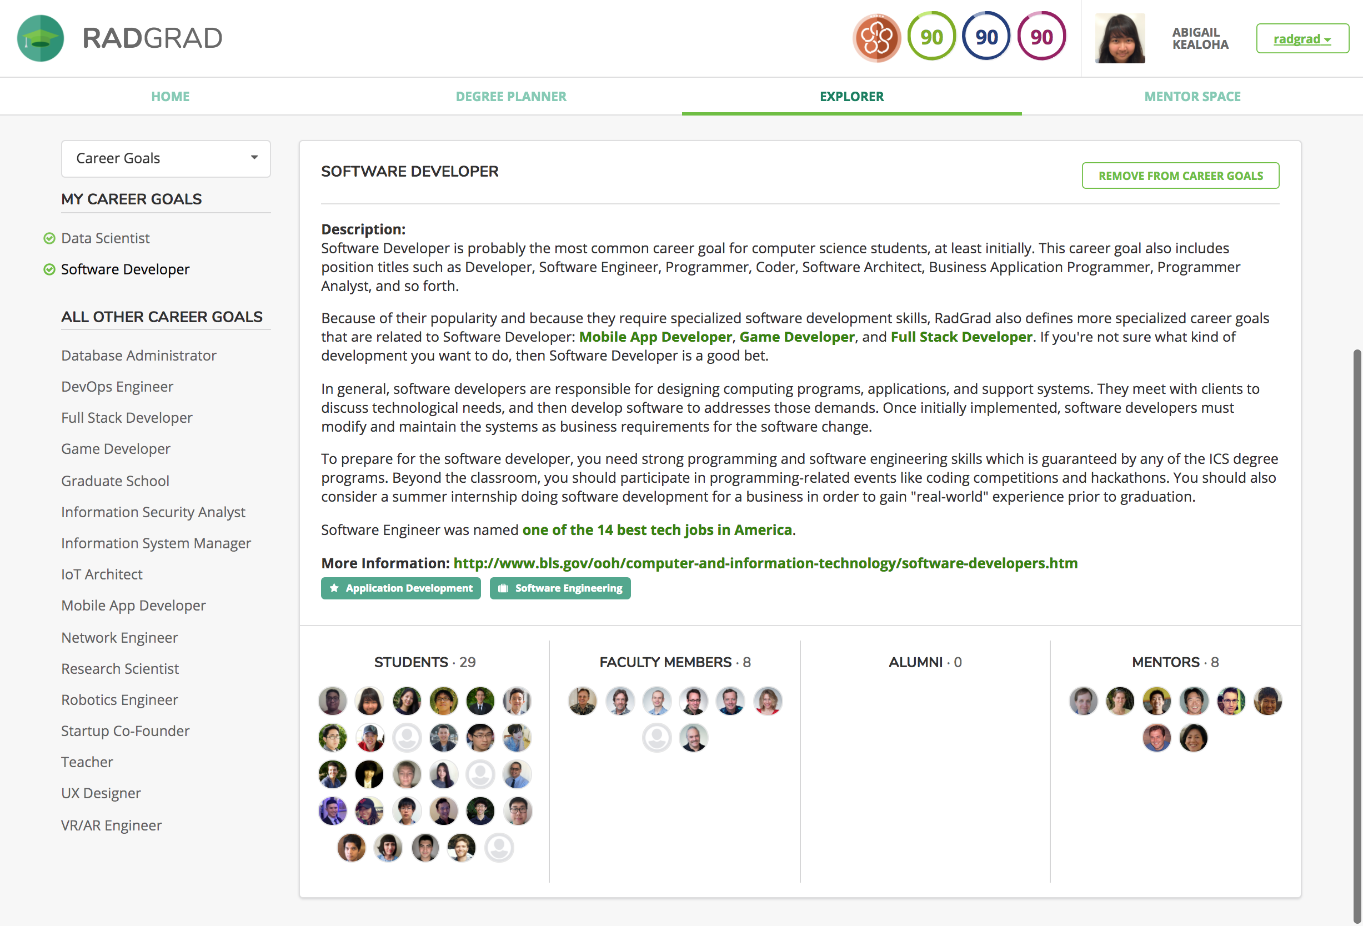
\includegraphics[width=1.0\textwidth]{careergoal-explorer}
\caption{Career Goal Explorer page.}
\end{figure}

\begin{figure}[h]
\centering
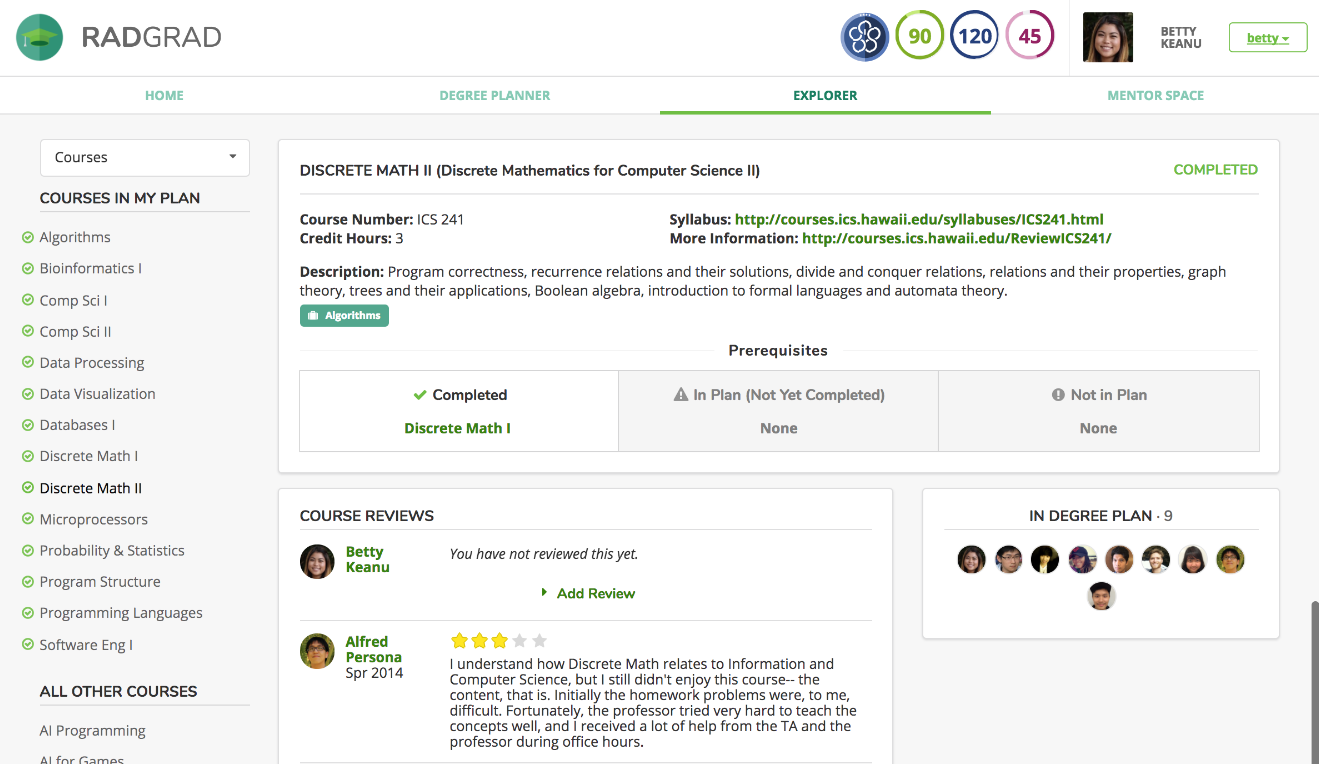
\includegraphics[width=1.0\textwidth]{course-explorer}
\caption{Course Explorer page.}
\end{figure}

\begin{figure}[h]
\centering
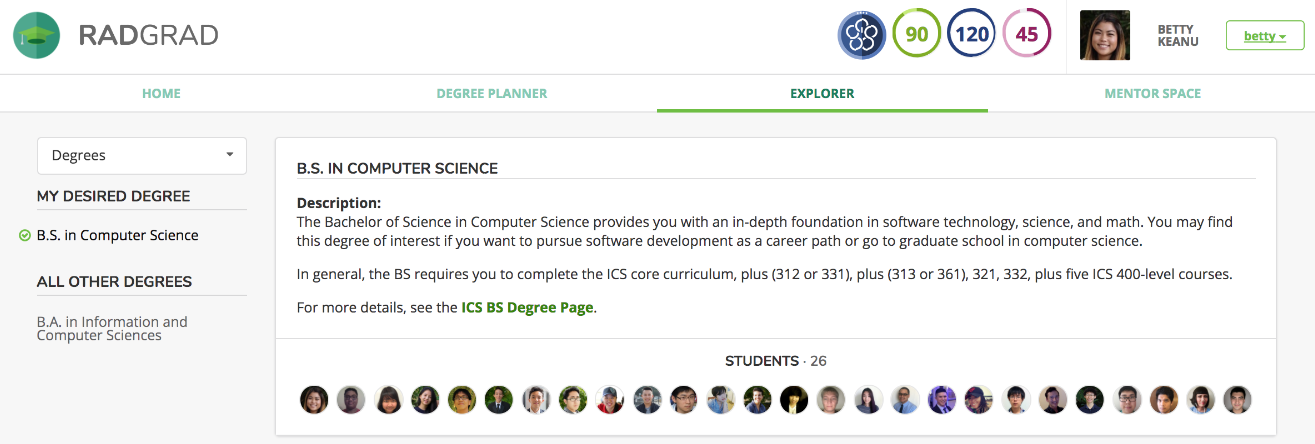
\includegraphics[width=1.0\textwidth]{degree-explorer}
\caption{Degree Explorer page.}
\end{figure}

\begin{figure}[h]
\centering
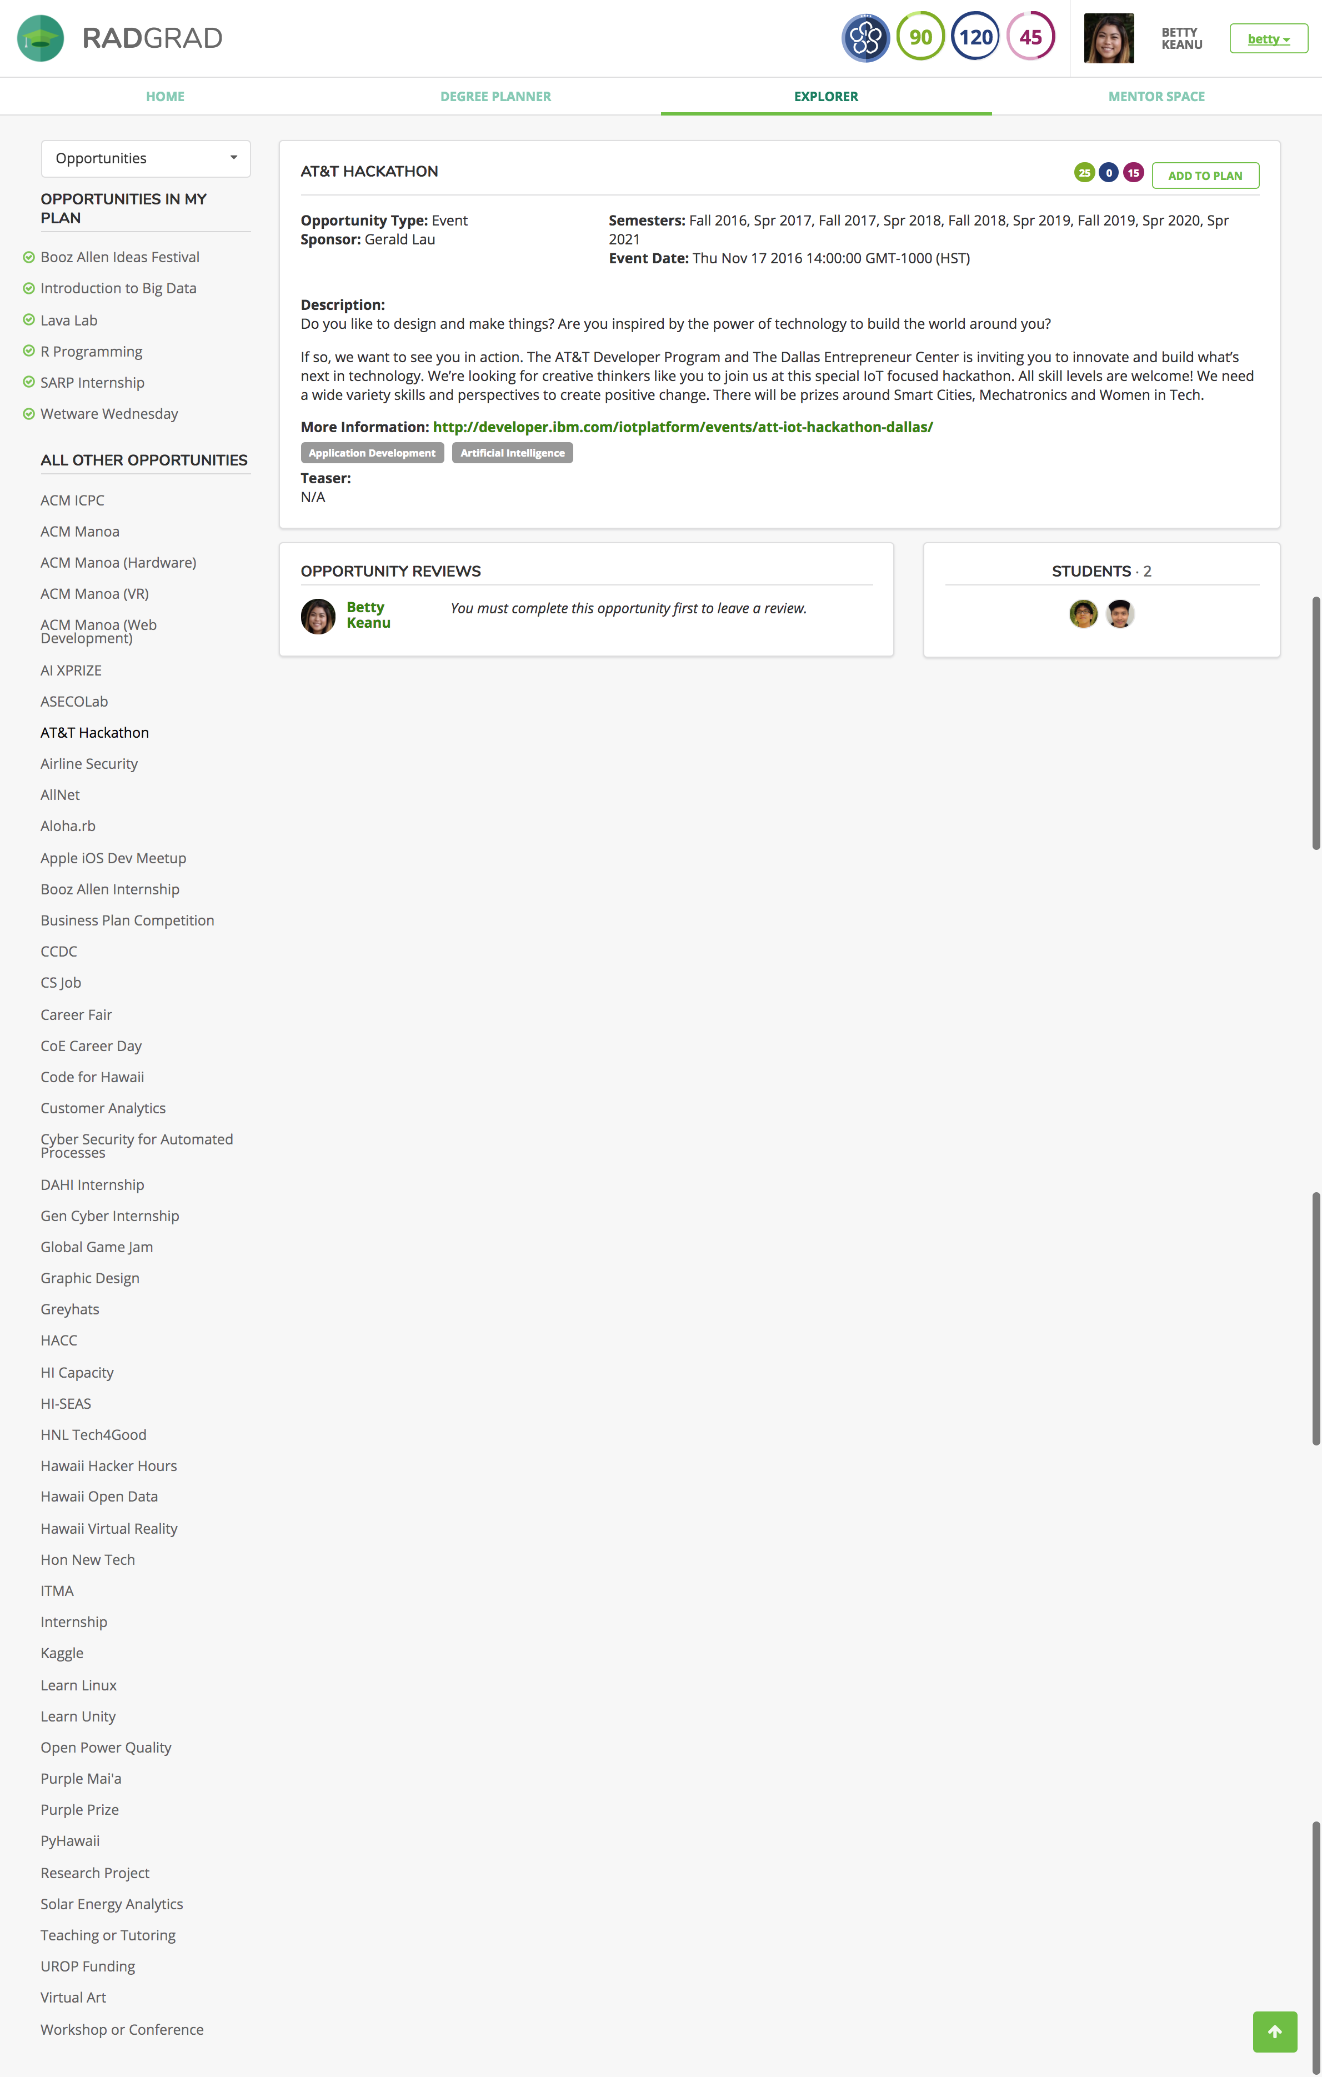
\includegraphics[width=1.0\textwidth]{opportunity-explorer}
\caption{Opportunity Explorer page.}
\end{figure}

Students can access the career goal, course, desired degree, and opportunity explorers to help them plan their degree.  These explorers can be accessed through the ``Explorer" top menu on the student home page. The specific explorer can be chosen using the dropdown menu on the left side. 

The career goal explorer lists all RadGrad career goals on the left side. These career goals are arranged by ``My Career Goals" (career goals that the user has added) and ``All other career goals" (career goals that the user has not added). The user can click on a career goal to view details about that career goal. These details include a description of the career goal, related interests, related courses and/or opportunities, a link for more information, interested students, interested faculty, interested alumni, and interested mentors. On this page, the user can also add or remove the career goal by clicking on the green button at the top right corner.  

The course explorer lists all RadGrad courses on the left side. These courses are arranged by ``Courses in my Plan" (all past, present or future courses in the student's degree plan) and ``All Other Courses" (courses not in the user's degree plan). The user can click on a course to view details about that course. These details include course number, a link to the syllabus, credit hours, a description of the course, prerequisites, organized into three categories (completed, in plan but not yet completed, and not in plan), and a list of students with this course in their degree plan. On this page, users can also view course reviews from other students and add or edit their own course review. The user can add or remove this course from their degree plan by clicking on the green button at the top right corner. If the user has already taken and passed the course, they cannot add it again.

The degree explorer lists all possible ICS degrees on the left side. These degrees are arranged by ``My Desired Degree" (the student can only have one desired degree at a time), and ``All Other Degrees" (degrees not currently chosen as the user's desired degree). The user can click on a degree to view details about that degree. These details include a description, where to go for more information, and a list of students who have this degree listed as their current desired degree. On this page, users can set a new degree goal by clicking on the green button at the top right corner.

The interest explorer lists all possible RadGrad interests on the left side. These interests are arranged by ``My Interests" (interests that the user has added), ``Career Goal Interests" (interests that have automatically been added due to their association with one or more of the user's chosen career goals), and ``All Other Interests" (interests that the user has not added and are not related to any of the user's career goals). The user can click on an interest to view details about that interest. These details include a description of the interest, related courses and related opportunities, both organized into three categories (completed, in plan but not yet completed, and not in plan), and students, faculty, alumni, and mentors who have added this interest. On this page, users can also add or remove the interest by clicking on the green button at the top right corner.

The opportunity explorer lists all ICS opportunities on the left side. These opportunities are arranged by ``Opportunities in my Plan" (all past, present or future opportunities in the user's degree plan) and ``All Other Opportunities" (opportunities not in the user's degree plan). The user can click on an opportunity to view details about that opportunity. These details include the opportunity type, semesters offered, event date, faculty sponsor, a description of the opportunity, related interests, a teaser video, and a list of students with this opportunity in their degree plan. On this page, users can also view opportunity reviews from other students and add or edit their own opportunity review. The user can add or remove this opportunity from their degree plan by clicking on the green button at the top right corner. Unlike courses, users can add an opportunity to their plan as many times as they would like.

\subsubsection{Teasers}
\begin{figure}[h]
\centering
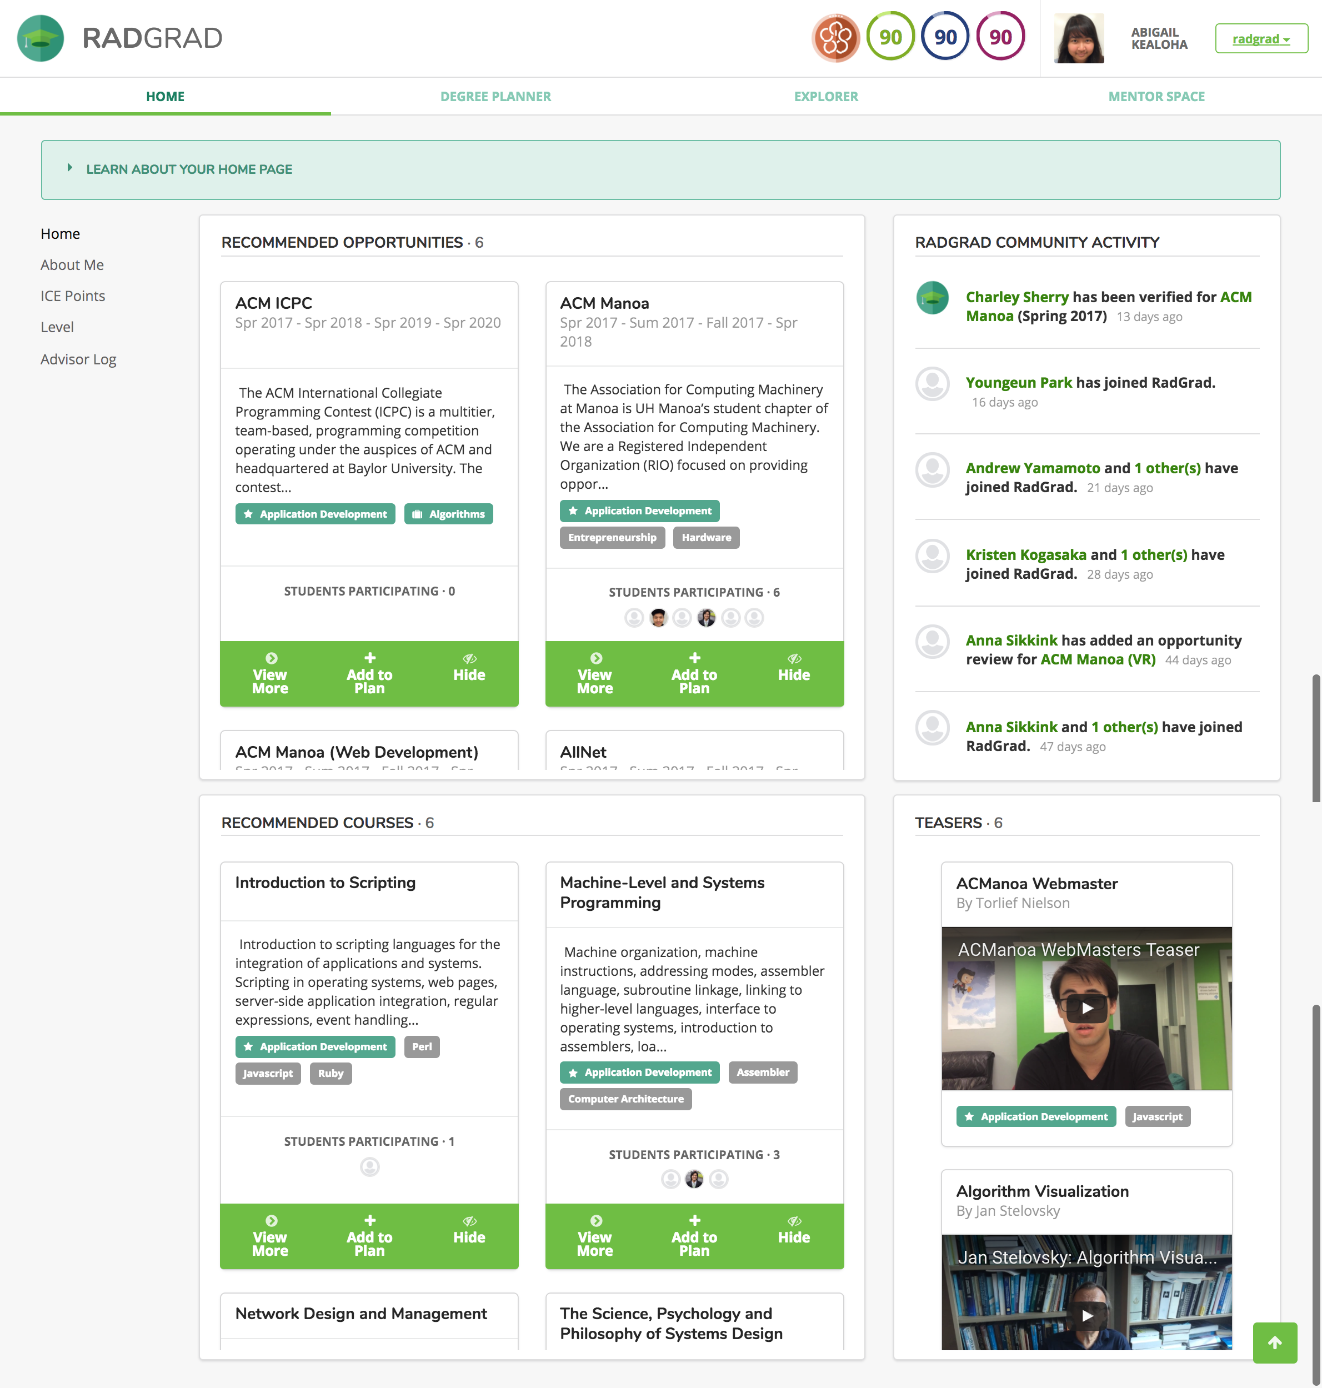
\includegraphics[width=1.0\textwidth]{student-home}
\caption{Student Home page with Teasers, Feed, and Recommended Courses and Opportunities.}
\end{figure}
Teasers are short (around 30 seconds) YouTube videos created by members of RadGrad to advertise their opportunity to the rest of RadGrad. Faculty members can create a teaser to help give students an idea of what their current research is about, and students can create a teaser to help give students an idea of what their club or event does and why other students should participate. These teasers supplement the textual opportunity descriptions in the explorer, and appear on the student's home page based off matching interests.

\subsection{Social Network}
\subsubsection{Avatars}
RadGrad quietly reminds users that they are not alone in using the system--they are part of a large and diverse network of real people. One of the ways RadGrad does this is by incorporating user avatars around the site. These avatars appear on the student home page, explorer pages, the user explorer, the student levels page, and the MentorSpace page. These avatars appear to show users related to a certain interest, career goal, course, opportunity, degree, and level. They also are associated with feed items, reviews, and MentorSpace answers. All avatars can be clicked on to navigate to the user's profile in the user explorer.  

\subsubsection{Feed}
Another way RadGrad reminds users that they are not alone in using the system is by providing a feed on the student home page. The feed is one of the first things that a user sees when they log in. Through this feed, users can see events occurring throughout RadGrad such as a new user joining RadGrad, a new course or opportunity is added on RadGrad, a user is verified for an opportunity, or a user has written a new course or opportunity review. The feed provides a single place for students to go to when they want to see what has changed since they have last logged in, and it constantly keeps students updated with the latest changes to the system. Since the feed also allows students to see what other students have been doing, they may be able to get a quick sense of what opportunities are popular among their classmates.

\subsubsection{Mentorspace}
\begin{figure}[h]
\centering
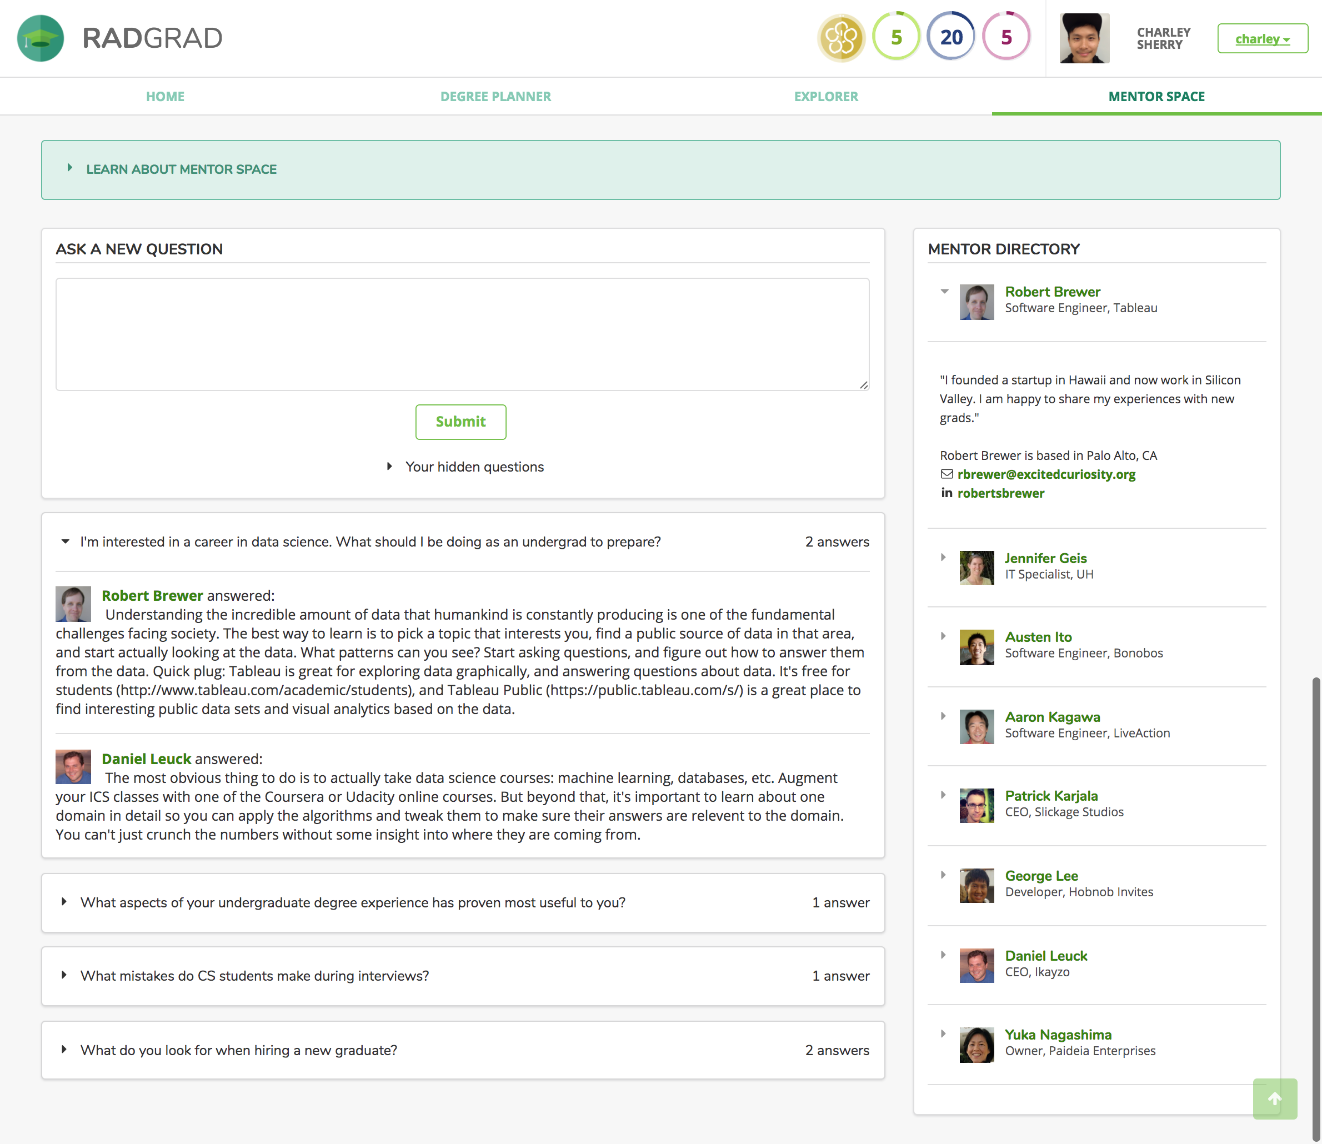
\includegraphics[width=1.0\textwidth]{mentor-space}
\caption{MentorSpace page.}
\end{figure}
Mentors and students can interact with each other on the MentorSpace page. The mentors are listed in the Mentor Directory on the right side of the page. Students can explore who the mentors are by expanding their profile and viewing information about their current company, current location, current job title, email address, LinkedIn, and a description about what inspired them to become a RadGrad mentor. On the left side of the page, students can submit new questions that they have for a mentor. Once the question has gone through moderation (by  Administrators), it will be posted on the MentorSpace for everyone to see. If a question is rejected, it can be edited and resubmitted as many times as desired. A question may be rejected if it contains profanity, is unclear, or is unrelated to ICS. Once a question is posted, mentors can leave an answer for the rest of the community to see. If a student has a specific question for a specific mentor, they can instead contact the mentor through the provided email rather than posting on MentorSpace, which is reserved for questions that can benefit the general ICS student community. 

\subsubsection{Advisor Log}
\begin{figure}[h]
\centering
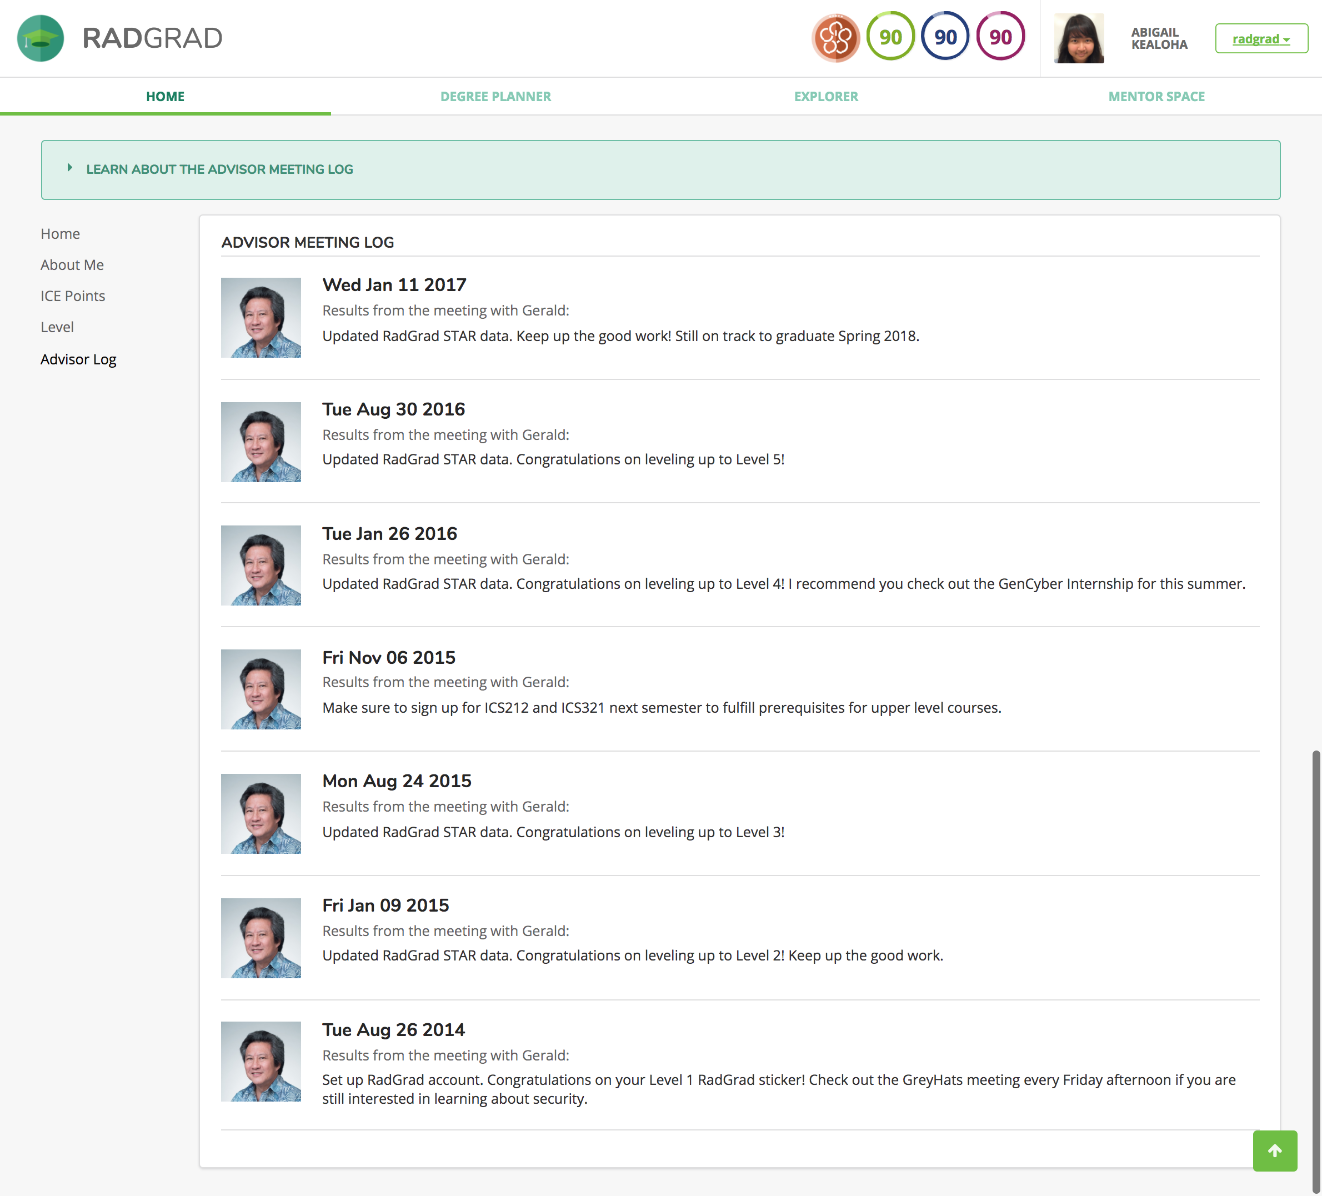
\includegraphics[width=1.0\textwidth]{advisor-log}
\caption{Student Advisor Log page.}
\end{figure}
Advisors and students can interact with each other on the Advisor Log page. When an advisor holds a meeting with a student, he can leave notes from the meeting on the student's Advisor Log. Each log includes a date, the name and avatar of the advisor, and the meeting notes. Advisors can use the log to keep track of their interactions with each student, and students can refer back to the log whenever they can't remember details about what their advisor had said. 

\subsubsection{Reviews}
Students can post two different types of reviews: course reviews and opportunity reviews. Students can leave reviews for a specific course or opportunity on the course or opportunity explorer page. Students can leave a 1-5 rating and reasons behind their rating. Students can edit or delete their review at any time. Any new or edited reviews immediately appear on the explorer page, but when they go through moderation, they may be removed if they do not abide by the guidelines. Reviews cannot be anonymous, which forces students to take full responsibility for whatever they decide to post. This, along with the fact that all users on RadGrad can view reviews, allows for full transparency between professors and students. Students can view other students reviews to get additional, first hand and anecdotal information about a course or opportunity before they decide to add it to their plan. Faculty and advisors can view reviews to gather feedback about how to improve the ICS program. 

\subsubsection{User Explorer}
\begin{figure}[h]
\centering
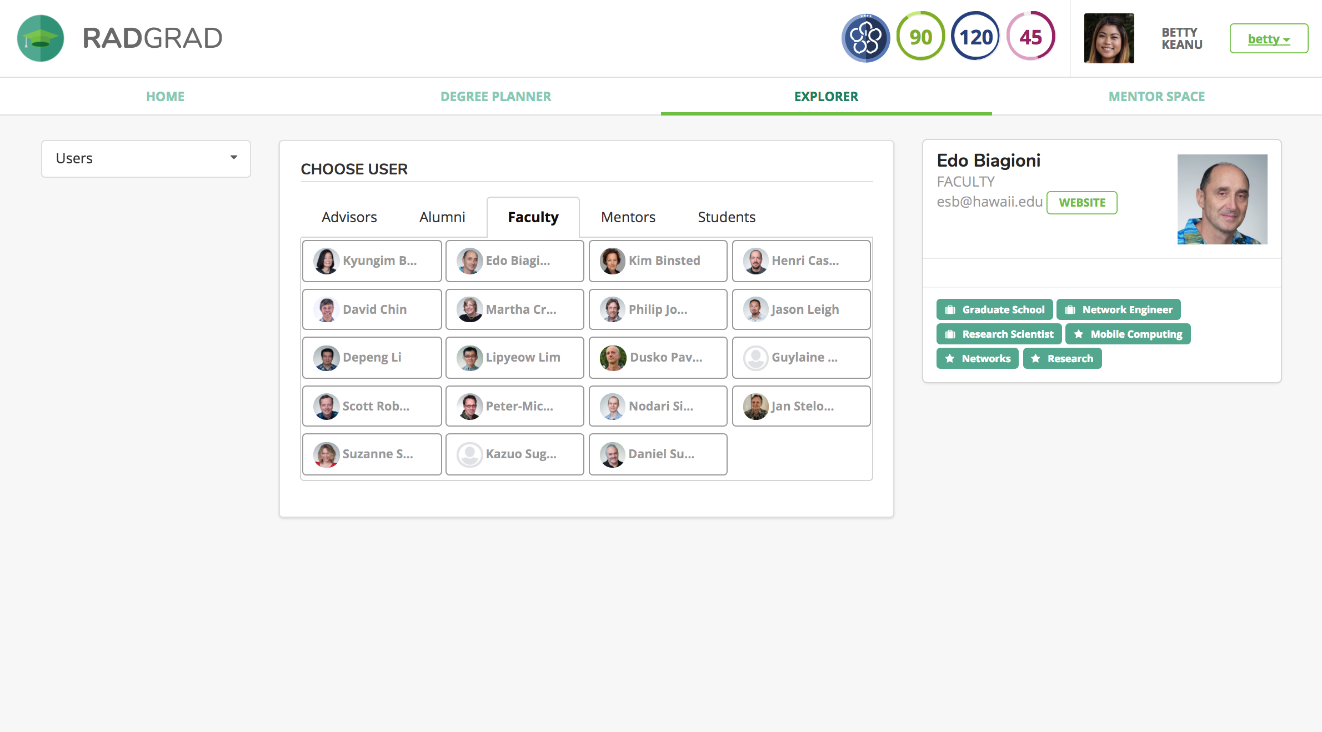
\includegraphics[width=1.0\textwidth]{user-explorer-faculty}
\caption{User Explorer page.}
\end{figure}

The user explorer lists all RadGrad users with their first name, last name, and avatar. Users are arranged in tabs by user type (Advisor, Alumni, Faculty, Mentor, Student) and then listed alphabetically by last name. The current user can click on a user to view details about that user. For student users, these details include desired degree, email, level, taken and planned courses, and completed and planned opportunities. For faculty users, these details include their email, a link to their website, and interests. For mentor users, these details include their email, their MentorSpace answers, and their interests. For advisor users, these details include their email and their interests. Students can use this explorer to learn more about other members of the RadGrad community, and figure out who might be beneficial to talk to (i.e. a higher level student with matching interests and interesting completed opportunities, or a faculty member with matching interests, or a mentor working at the student's dream company).

\subsection{Gamification}
\subsubsection{ICE}
\begin{figure}[h]
\centering
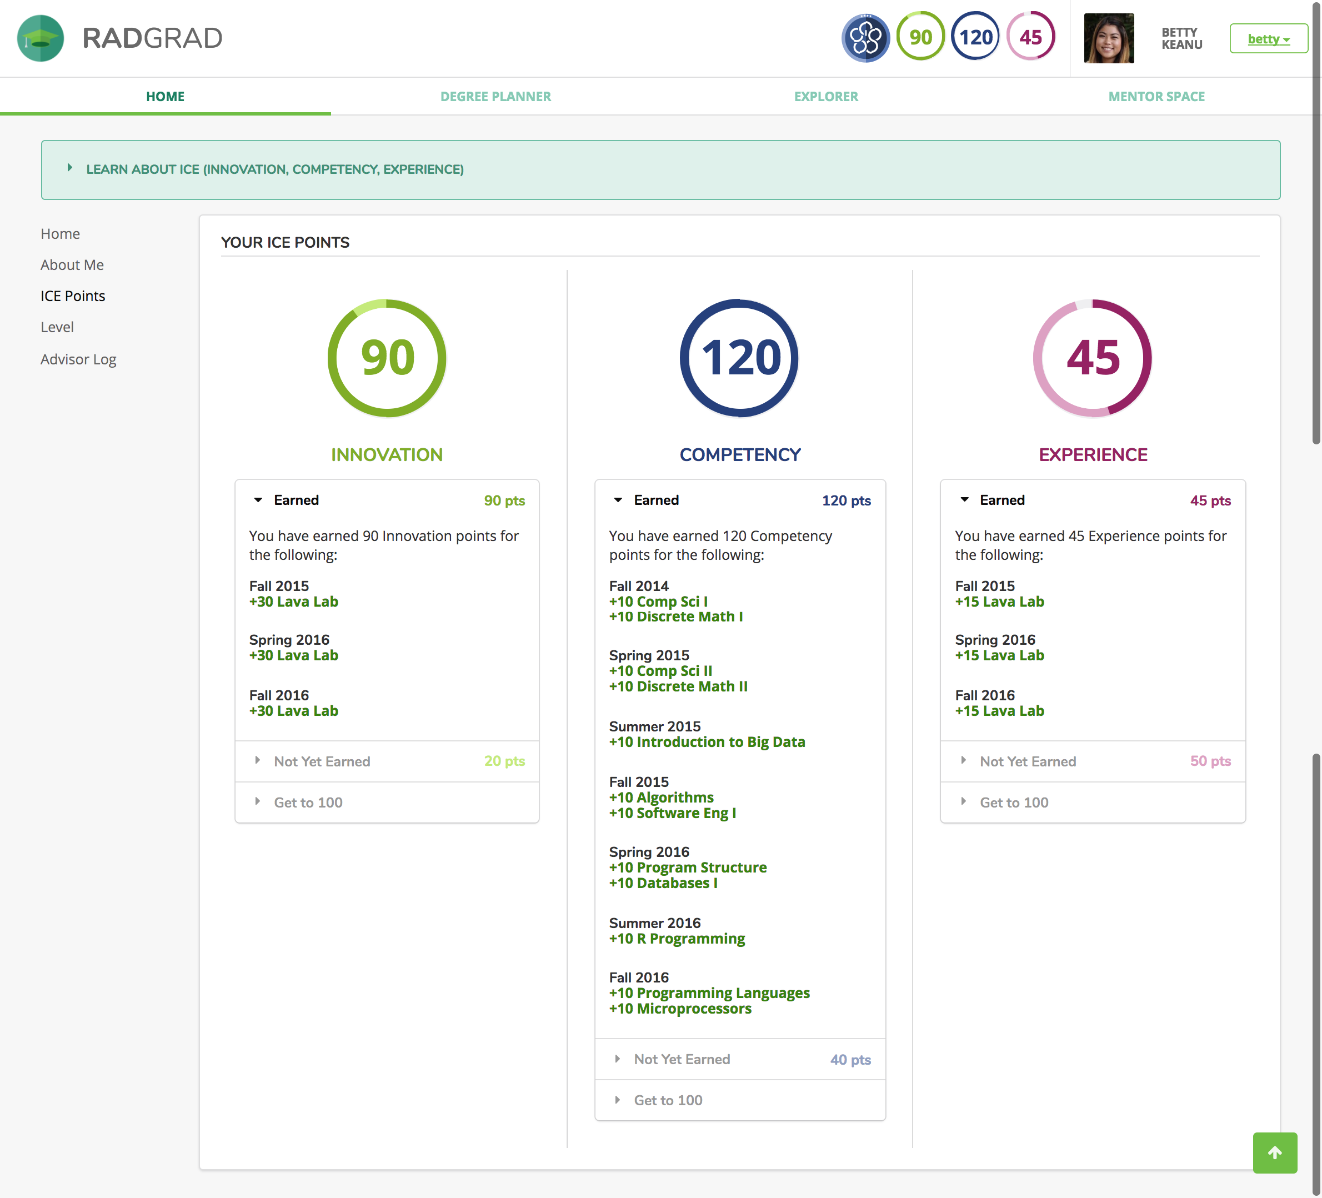
\includegraphics[width=1.0\textwidth]{student-ice}
\caption{ICE page.}
\end{figure}

The student ICE page displays three circular graphs: one each for innovation, competency, and experience. The number in the center of each graph represents the current amount of points earned for that category. The dark fill in the graph represents the same number. The light fill on the graph represents the amount of planned points. In addition to the student ICE page, these ICE graphs also appear in the top right corner of the menu bar. 

ICE points are also represented for specific courses or opportunities. These ICE points are represented using three filled circles: one each for innovation, competency, and experience. Each circle has a number in the center which represents the amount of points that course or opportunity is worth for that particular ICE category. Students can use these ICE representations to decide which courses or opportunities they should add to their plan, in order to improve their ICE score. These representations appear on the degree planner inspector pane and in the course and opportunity explorer pages. 

\subsubsection{Levels}
\begin{figure}[h]
\centering
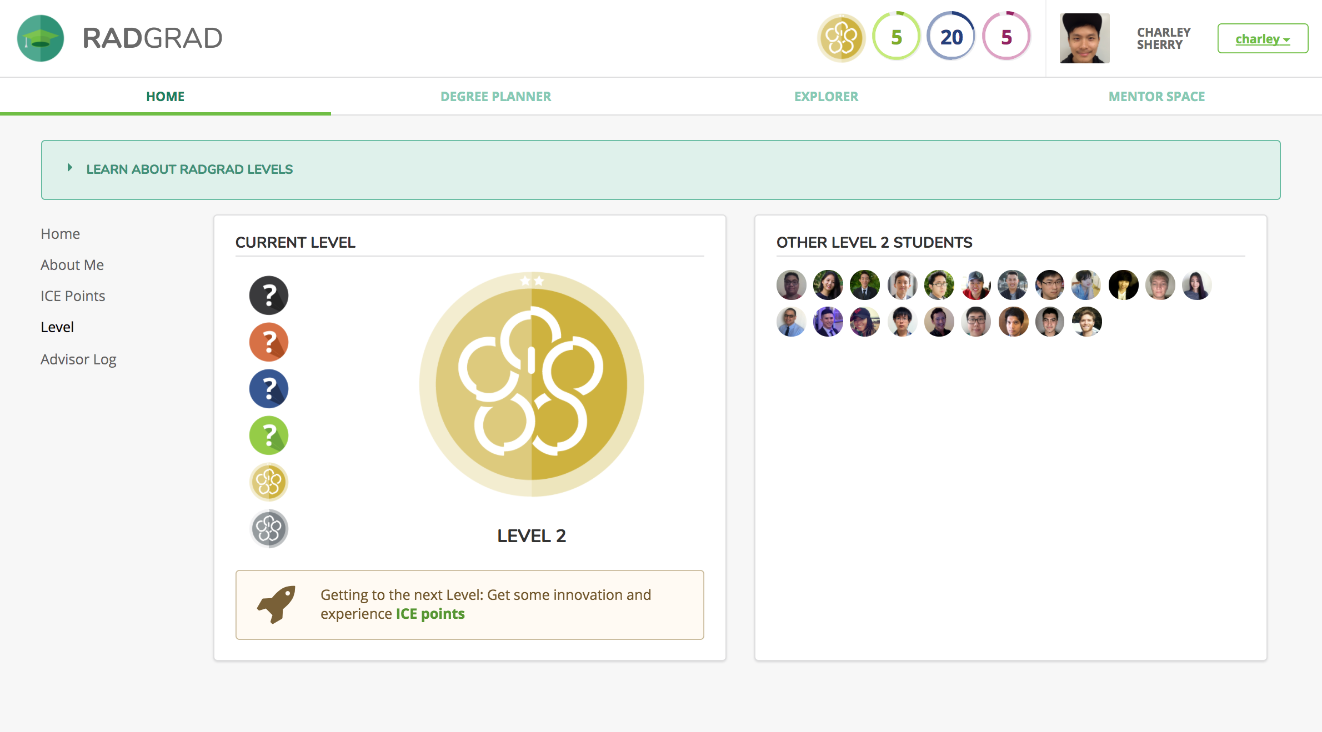
\includegraphics[width=1.0\textwidth]{levels}
\caption{Levels page.}
\end{figure}

Students can view their current level badge on the student level page. This page also includes leveling up hints and a list of other students who are at the same level (listed with avatars). 

Levels also persist physically off of RadGrad in the form of stickers. These stickers can be obtained from an advisor or a RadGrad administrator, and a student will receive a new sticker each time they achieve a new level. Students are encouraged to display these stickers on their laptop, as a subtle way to communicate their current standing to their classmates. Using these stickers, students can more easily identify students who are at the same level as them to mingle with, identify students at a higher level than them to get advice from, and identify students at a lower level who could use some peer mentoring. These stickers can also be used to identify current or former ICS students while off campus. In this way, these physical manifestations of RadGrad help to create a sense of ICS community offline as well. 

\section{Advisor Mode}
\subsection{Student Configuration}
\begin{figure}[h]
\centering
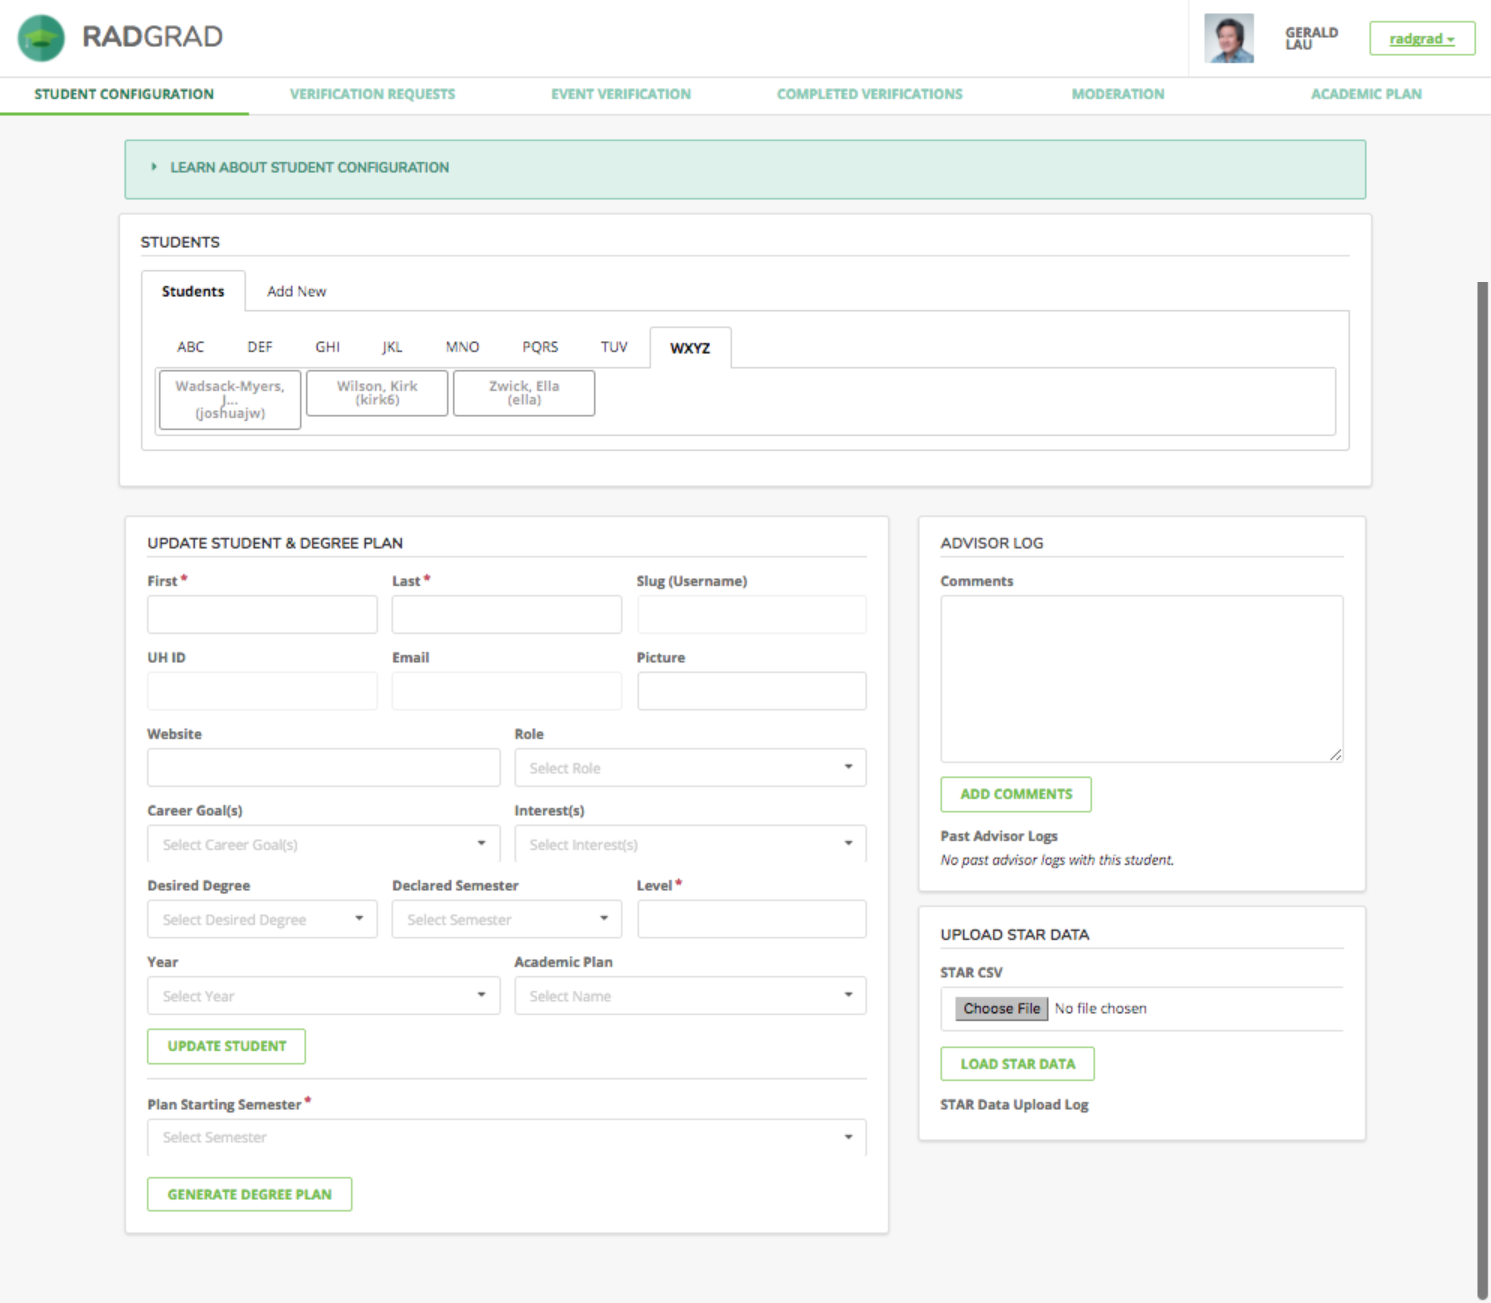
\includegraphics[width=1.0\textwidth]{advisor-student-configuration}
\caption{Advisor student configuration page.}
\end{figure}
On the student configuration page, advisors can add new students or update existing students. Existing students are listed alphabetically by last name. Advisors can update a student's first name, last name, picture, website, role, career goals, interests, desired degree, declared semester, level, year, academic plan, and plan starting semester from this interface. (Slug, email, and UH ID cannot be changed once the student has been added to RadGrad). On this page, advisors can also add advisor log comments and view any past advisor logs for a particular student. Advisors can also use this page to upload new star data and view past star data uploads. 
\subsection{Verification}
Advisors can verify a student's completion of an opportunity in two ways: with a pending verification, and with an event verification. If an advisor is physically at an event, and needs to quickly verify a large amount of students, he can use the event verification. In this interface, the advisor simply chooses the event from a dropdown selection of recent events, and then types in the student's UH account name and clicks ``Verify Attendance." If an advisor is not physically present, a student can send a verification request through RadGrad. These requests show up as pending verifications. Advisors can choose to accept or decline these verifications. If they decide to decline, they can leave feedback for the student, and the student can resubmit as many times as they choose. Adivsors can view Completed Verifications to either simply check past verifications or to reopen a verification.
\subsection{Moderation}
\begin{figure}[h]
\centering
\includegraphics[width=1.0\textwidth]{advisor-moderation}
\caption{Advisor Moderation Page.}
\end{figure}
Advisors can use the moderation page to moderate course reviews, opportunity reviews, and MentorSpace questions. Advisors can choose to either accept or deny these posts. In the case of denial, advisors can leave reasons for denial so that the student can edit and resubmit their post accordingly. 
\subsection{Academic Plan}
\begin{figure}[h]
\centering
\includegraphics[width=1.0\textwidth]{advisor-academic-plan}
\caption{Advisor Academic Plan Page.}
\end{figure}
The academic plan page is the only place on RadGrad that allows the user to build academic plans. There are two tabs: Viewer and Builder. The viewer allows the advisor to choose a year and a plan name, and view the four year plan for that plan. To make any edits to an existing plan or add a new plan, advisors can go over to the builder, which allows them to name a new academic plan with a degree, name, and year. The advisor can then build the four year plan easily by dragging and dropping possible courses onto the initially empty plan. Some plans have more complex requirements than a single courses (i.e. a student must take one course from one of the four groups: ICS312 or ICS331, ICS 313 or ICS361, ICS351 or ICS451, or ICS355). For requirements like this, advisors can easily create groupings by dragging courses to the box with the link icon. Once a complex requirement is completely built, it can be dragged directly onto the plan. If an advisor no longer needs a certain requirement, they can delete it by dragging it to the trash can icon. 

\section{Faculty Mode}
\subsection{Profile}
\begin{figure}[h]
\centering
\includegraphics[width=1.0\textwidth]{faculty-profile}
\caption{Faculty profile page.}
\end{figure}
Faculty can use the profile page to view and edit their profile, which reflects how others will see them on RadGrad. On this page, faculty can update their photo and information about their website. Faculty can personalize their profiles in a way that accurately communicates their background and research to students. 
\subsection{Manage Opportunities}
\begin{figure}[h]
\centering
\includegraphics[width=1.0\textwidth]{faculty-opportunity}
\caption{Faculty Manage Opportunities page.}
\end{figure}
Faculty can use the manage opportunities page to easily view, add, edit, or delete their sponsored opportunities. They can also view other opportunities, but they can only edit their own. Faculty can edit their opportunities at any time.
\subsection{Verification}
\begin{figure}[h]
\centering
\includegraphics[width=1.0\textwidth]{faculty-verification}
\caption{Verification Page.}
\end{figure}

\begin{figure}[h]
\centering
\includegraphics[width=1.0\textwidth]{faculty-pending-verification}
\caption{Pending Verifications Page.}
\end{figure}
Faculty have the same verification interface as advisors, except they can only view their own verifications for their own sponsored opportunities. 
\subsection{Explorers}
Faculty view the same explorer as students, except they cannot add courses or opportunities, and they cannot leave any type of review. However, they can use the explorer to add interests and career goals. Also, the opportunity explorer conveniently shows the faculty's sponsored opportunities at the top of their opportunity list for quick access.

\section{Mentor Mode}
\subsubsection{Profile}
\begin{figure}[h]
\centering
\includegraphics[width=1.0\textwidth]{mentor-profile}
\caption{Mentor profile page.}
\end{figure}
Mentors can use the profile page to view and edit their profile, which reflects how others will see them on RadGrad. On this page, mentors can update their photo and information about their website, company, job title, location, LinkedIn, and motivation for becoming a mentor. Mentors can personalize their profiles in a way that accurately communicates their background and willingness to help to the students. 
\subsubsection{MentorSpace}
\begin{figure}[h]
\centering
\includegraphics[width=1.0\textwidth]{mentor-mentorspace}
\caption{Mentor MentorSpace Page.}
\end{figure}
Mentors view the same MentorSpace that students do, except each question has an ``Answer this question" or ``Edit your answer" button. Clicking on this button brings up a form at the top of the page, which mentors can use to either submit a new answer or revise their existing answer. 
\subsubsection{Explorer}
Mentors view the same explorer as students, except they cannot add courses or opportunities, and they cannot leave any type of review. However, they can use the explorer to add interests and career goals.

\section{Administrator Mode}
\subsection{Retrieve User}
\begin{figure}[h]
\centering
\includegraphics[width=1.0\textwidth]{admin-retrieve-user}
\caption{Administrator Retrieve User page.}
\end{figure}
On the Administrator home page, an administrator can access any user's account. Users are organized by role (on tabs) and then alphabetically by last name. Clicking on the user's name will lead to their profile. Administrators can use this for testing or troubleshooting purposes. On the student tab, there is also a button to update student levels. Clicking this button will automatically recalculate and set the levels for all of the students.

\subsection{Data Model}
\begin{figure}[h]
\centering
\includegraphics[width=1.0\textwidth]{admin-datamodel}
\caption{Administrator Data Model page.}
\end{figure}
The data model page allows administrators to view, add, edit, and delete items from the data model. The menu on the left lists all collections. When an administrator clicks on a collection, they will see a form, which they can use manipulate items in that collection. Below the form, they can view a list of all existing collection items. 
\subsection{Data Base}
\begin{figure}[h]
\centering
\includegraphics[width=1.0\textwidth]{admin-database}
\caption{Administrator Data Base page.}
\end{figure}
The database page allows administrators to easily run an integrity check on the database, dump the database, and restore the database. The integrity check tests every item in the database to make sure that all parts of it are valid. Dumping the database saves the current state of the database to a JSON file and downloads it to your computer. Restoring the database deletes the current database and reloads an earlier version from a JSON file. Administrators can use this in backup and testing situations.
\subsection{Moderation}
Administrators have the same moderation page as advisors. 
\chapter{Conclusions}
The main goal of this thesis is to find evidence of a problem, gather more concrete evidence of this problem, and attempt to solve the problem with the initial design and implementation of a system. When I initially gathered TechHui data about the pros and cons of being an ICS student at UH Manoa, I found the first evidence of a problem: over the past eight years, students were not fully satisfied with the ICS experience. I then designed and implemented an ICS experience survey, which surveyed 100 current ICS students and asked more specific questions about their ICS experience. The results of this survey gave more concrete evidence that there is room for improvement in the ICS department when it comes to encouraging and enabling students to participate in extracurricular activities, giving students the support they need from all members of the department, and encouraging and enabling students to interact with each other and ICS alumni on an academic or professional level. Along with the rest of the RadGrad team, I have helped to design and implement a system called RadGrad, which aims to address many perceived deficiencies within the ICS department. By combining degree planning, social networking, and gamification, RadGrad aims to improve the ICS student experience on academic, professional, and social levels. 

With the current implemented features, RadGrad aims to solve the following five out of the ten categories from the TechHui data. The social networking features aim to solve numbers 1, 4, and 5. The review feature has the potential to solve number 2. The degree planner system, interests, career goals, and opportunities will help students become more aware of the degree focuses that are offered, and allows students to create their own customized ICS experience based off their own interests and career goals, which solves number 3. Although RadGrad doesn't currently address all of the problems that students have, it could potentially cover more issues in future deployments. 

\begin{enumerate}
  \item The ICS department needs a better sense of community.
  \item Some of the professors in the ICS department need to improve their teaching.
  \item The ICS department should offer more focused areas of study.
  \item ICS courses should involve more group work 
  \item ICS should encourage more interaction among students.
\end{enumerate}

After completing this thesis, RadGrad development will continue, and is scheduled to be deployed within the ICS department in Fall 2017. Future studies will be necessary to test whether or not RadGrad is adequately addressing problems within the department. After students have integrated RadGrad into their life for at least one semester (the time needed to go through once registration process and have enough time to participate in opportunities and courses), future studies may want to conduct another survey with ICS students. This survey could include similar questions to the survey conducted in my survey, which can then be used to compare and contrast pre- and post-RadGrad results. This survey could also include more RadGrad specific questions, to get an idea of how students feel about using the system. Furthermore, gathering usage statistics could possibly add valuable insight into how users are actually responding to and interacting with the system. Based on the results of these studies, RadGrad could either be further improved to better solve the perceived problems, or discarded if there is no evidence that RadGrad has any positive impact on the ICS community.

Assuming that RadGrad is successful within the ICS department, future possible expansions include integration into other departments at UH Manoa, being established as a staple UH system that will get its own funding and staff positions, being integrated at other universities, and finally being integrated in other environments, such as within tech companies. 

This thesis marks the beginning of the RadGrad journey, and will hopefully be the first of many studies. After completing this thesis, the overall results suggest that RadGrad is progressing in a promising direction, and if it continues on that path, it will have the potential to positively revolutionize the lives of future students in many different ways.   

%%% Switch to appendix mode
\appendix

%%% Bring in any appendices from external file (optional)
%%%%%%%%%%%%%%%%%%%%%%%%%%%%%% -*- Mode: Latex -*- %%%%%%%%%%%%%%%%%%%%%%%%%%%%
%% uhtest-appendix.tex -- 
%% Author          : Robert Brewer
%% Created On      : Fri Oct  2 16:31:12 1998
%% Last Modified By: Robert Brewer
%% Last Modified On: Mon Oct  5 14:41:05 1998
%% RCS: $Id: uhtest-appendix.tex,v 1.1 1998/10/06 02:07:03 rbrewer Exp $
%%%%%%%%%%%%%%%%%%%%%%%%%%%%%%%%%%%%%%%%%%%%%%%%%%%%%%%%%%%%%%%%%%%%%%%%%%%%%%%
%%   Copyright (C) 1998 Robert Brewer
%%%%%%%%%%%%%%%%%%%%%%%%%%%%%%%%%%%%%%%%%%%%%%%%%%%%%%%%%%%%%%%%%%%%%%%%%%%%%%%
%% 

\chapter{Baseline Assessment}
\label{baseline-assessment}
\begin{figure}[h]
\centering
\includegraphics[width=0.75\textwidth]{q1}
\caption{Baseline Assessment: Section 1.}
\end{figure}

\begin{figure}[h]
\centering
\includegraphics[width=0.75\textwidth]{q2}
\caption{Baseline Assessment: Section 2.}
\end{figure}

\begin{figure}[h]
\centering
\includegraphics[width=0.75\textwidth]{q3}
\caption{Baseline Assessment: Section 3.}
\end{figure}

\begin{figure}[h]
\centering
\includegraphics[width=0.75\textwidth]{q4}
\caption{Baseline Assessment: Section 3.}
\end{figure}

\begin{figure}[h]
\centering
\includegraphics[width=0.75\textwidth]{q5}
\caption{Baseline Assessment: Section 3.}
\end{figure}

\begin{figure}[h]
\centering
\includegraphics[width=0.75\textwidth]{q6}
\caption{Baseline Assessment: Section 4.}
\end{figure}

\begin{figure}[h]
\centering
\includegraphics[width=0.75\textwidth]{q7}
\caption{Baseline Assessment: Section 4.}
\end{figure}

\begin{figure}[h]
\centering
\includegraphics[width=0.75\textwidth]{q8}
\caption{Baseline Assessment: Section 5.}
\end{figure}

\chapter{RadGrad Data Model}
\label{data-model}
\subsection{Career Goals}
\begin{figure}[htbp!]
\centering
\includegraphics[width=1.0\textwidth]{dm-career}
\caption{Example of a career goal representation.}
\label{career-goal}
\end{figure}
Career goals represent possible ICS related careers that ICS students can aspire to get after graduation (Figure 6.1). Each career goal has an associated name, slug, description, related interests, and an optional URL for more information. Students can choose as many career goals as they want. Faculty and mentors can choose career goals that they would like to be associated with as well. Possible career goals as of June 2017 are listed in Table ~\ref{table:career-goals}.

\begin{table}[htbp!]
\centering
\begin{tabular}{ l l l } 
 Data Scientist & Database Administrator & DevOps Engineer \\ 
 Full Stack Developer & Game Developer & Graduate School \\ 
 Information Security Analyst & Information System Manager & IoT Architect \\ 
 Mobile App Developer & Network Engineer & Research Scientist \\
 Robotics Engineer & Software Developer & Startup Co-Founder \\
 Teacher & UX Designer & VR/AR Engineer 
\end{tabular}
\caption{List of RadGrad career goals as of June 2017}
\label{table:career-goals}
\end{table}

\subsection{Courses}
\begin{figure}[htbp!]
\centering
\includegraphics[width=1.0\textwidth]{dm-course}
\caption{Example of a course representation.}
\label{course}
\end{figure}
Courses represent all past, present, and future ICS courses (Figure ~\ref{course}). Each course has an associated name, short name, slug, course number, description, credit hours, related interests, a syllabus URL, a URL for more information, and associated prerequisites. The course name is the official name appearing in the UH registration guide, and the course short name is used for display purposes. Students may add as many courses as they would like to their degree plan. 

Course instances represent individual instances for each student. Each course instance has an associated semester, course, whether it has been verified or not, whether it came from STAR or not, grade, credit hours, note, student, and associated ICE points. A past course instance is always considered verified if it is from STAR. Course instances from STAR from the current or future semesters are not considered verified yet since there is no official grade. Special courses that are manually input (not from STAR) could also be considered verified by an advisor. A course instance has a note if it is not an ICS course. It is important to note that course instances on RadGrad are only valid on RadGrad, and students must use other methods to officially make UH course registration changes.

\subsection{Desired Degrees}
\begin{figure}[htbp!]
\centering
\includegraphics[width=1.0\textwidth]{dm-degree}
\caption{Example of a desired degree representation.}
\label{desired-degree}
\end{figure}
Desired degrees represent all past, present, and future ICS degrees (Figure ~\ref{desired-degree}). Each desired degree has an associated name, short name, slug, and description. Students can only choose one desired degree at any given time. However, they are free to switch desired degrees as many times as they want. It is important to note that desired degrees on RadGrad are only valid on RadGrad, and students must use other methods to officially change their declared degree at UH. 

\subsection{Degree Plan}
\begin{figure}[htbp!]
\centering
\includegraphics[width=1.0\textwidth]{dm-degreeplan}
\caption{Example of a degree plan representation.}
\label{degree-plan}
\end{figure}
Degrees plans represent all past, present, and future ICS degree plans (Figure ~\ref{degree-plan}). Each degree plan has an associated degree, name, effective semester, amount of courses per semester, and list of courses. Students can view degree plans if they would like a more specific focus than just a broad BS or BA degree. Examples of degree plans are ``BS in Computer Sciences Security Sciences", ``BA in ICS Security Science Focus", and ``BA in Computer Sciences IT Focus." Students can look at any plan at any time to see what they would need to do to fulfill it. It is important to note that these degree plans change over time, and a ``BS in Computer Sciences Security Sciences" may be different in 2016 than in 2018. This is why both year and plan name must be chosen when selecting a plan.  Degree plans were created to help students to become more aware of and make sense of the different degree plans that they can choose from. Having these representations on RadGrad help students to see how different degree plans would work with their specific interests, career goals, courses, and opportunities. Overall, degree plans can help students to narrow down their interests into a more specific field. 

\subsection{Feeds}
\begin{figure}[htbp!]
\centering
\includegraphics[width=0.5\textwidth]{dm-feed}
\caption{Example of a feed representation.}
\label{feed}
\end{figure}
Feeds represent select actions of RadGrad users (Figure ~\ref{feed}). Each feed has associated users, opportunity, course, semester, description, time stamp of the action, picture, and feed type. A feed could have one or multiple users. There are currently six different feed types: a new RadGrad user is added, a new course is added to RadGrad, a new opportunity is added to RadGrad, a user has been verified for completing an opportunity, a new course review has been added, and a new opportunity review has been added. These particular actions have been selected because they could be useful and of interest to other RadGrad users.

\subsection{Feedbacks}
\begin{figure}[htbp!]
\centering
\includegraphics[width=1.0\textwidth]{dm-feedback}
\caption{Example of feedback representations.}
\label{feedback}
\end{figure}
Feedbacks represent recommendations and warnings for students (Figure ~\ref{feedback}). Each feedback has an associated name, slug, description, and feedback type. There are currently two feedback types: recommendation and warning. 

Feedback instances represent individual instances for each student. Each feedback instance has an associated feedback, user, description, and area. There are currently four different areas: interests, ICE, STAR, and degree plan. Each time the student's plan changes, feedback instances in these areas are deleted and recalculated.

\subsection{Help Messages}
\begin{figure}[htbp!]
\centering
\includegraphics[width=1.0\textwidth]{dm-help}
\caption{Example of a help representation.}
\label{help}
\end{figure}
Help messages represent guidance for a particular RadGrad page (Figure ~\ref{help}). Each help message has an associated route name, title, and text. The text can contain actual text, images, and formatting. Each page (route name) can have at most one help message. These help messages are displayed at the top of the specified page, in a collapsible pane.  

\subsection{ICE}
\begin{figure}[htbp!]
\centering
\includegraphics[width=1.0\textwidth]{dm-ice}
\caption{Example of an ICE representation.}
\label{ice}
\end{figure}
ICE represents a student's ICE points (Figure ~\ref{ice}). Each ICE has an associated number for ``I", ``C", and ``E." There are two types of ICE points: earned and planned. Earned ``I" and ``E" points are calculated by adding the ``I" or ``E" points for each verified opportunity in the student's plan. Earned ``C" points are calculated by adding the ``C" points for each verified course in the student's plan. The amount of earned points for each course depends on the grade that the student received; A's represent more points than B's. Planned ``I" and ``E" points are calculated by adding the ``I" or ``E" points for each unverified opportunity in the student's plan. Planned ``C" points are calculated by adding the ``C" points for each unverified course in the student's plan. A student's earned and planned ICE points are updated each time there are changes to the student's degree plan. 

\subsection{Interests}
\begin{figure}[htbp!]
\centering
\includegraphics[width=1.0\textwidth]{dm-interests}
\caption{Example of an interest representation.}
\label{interests}
\end{figure}
Interests represent possible ICS related interests that RadGrad users could have (Figure ~\ref{interests}). Each interest has an associated name, slug, description, interest type, and a URL for more information. All RadGrad users may choose to be associated with as many interests as they would like. All current interests on RadGrad as of June 2017 are listed in Table ~\ref{table:interests}.

\begin{table}[htbp!]
\centering
\begin{tabular}{ l l l } 
.NET & Algorithms & Android \\ 
Application Development & Artificial Intelligence & Assembler \\
Bioinformatics & Biology & C and C++ \\
C\# & Civic Engagement & Cognitive Science \\
Computer Architecture & Computer Ethics & Computer Graphics \\
Computer Vision & Cryptography & Data Science \\
Data Visualization & Databases & Entrepreneurship \\
Game Design & Graphic Design & Hardware \\
High Performance Computing & Human-Computer Interaction & IT Management \\
Java & Javascript & Linux \\
Lisp & Machine Learning & Mobile Computing \\
Networks & Operating Systems & Parallel Programming \\
Perl & Prolog & Psychology \\
Python & R & Research \\
Robotics & Ruby & Software Development \\
SQL & Security & Sustainability \\
Teaching & Theory of Computation & Unity \\
Virtual Reality & Web Development & iOS
\end{tabular}
\caption{List of RadGrad interests as of June 2017}
\label{table:interests}
\end{table}

\subsection{Levels}
\begin{figure}[htbp!]
\centering
\includegraphics[width=0.5\textwidth]{dm-level}
\caption{Example of a level representation.}
\label{levels}
\end{figure}
Levels represent a student's RadGrad level (Figure ~\ref{levels}). There are six possible levels, from Level 1 to Level 6. A student's level is calculated based off the amount of ICS courses they have passed, the amount of opportunities they have done, and the amount of reviews they have contributed on RadGrad. Levels can be recalculated for all users at any time through the administrator pages.

\subsection{Advisor Logs}
\begin{figure}[htbp!]
\centering
\includegraphics[width=1.0\textwidth]{dm-log}
\caption{Example of an advisor log representation.}
\label{log}
\end{figure}
Advisor logs represent an interaction between an ICS advisor and a student (Figure ~\ref{log}). Each advisor log has an associated student, advisor, text, and date created. A new log can be created by the advisor whenever they have a meeting with a student. Advisors and students can use these logs to keep track of when meetings were held, and what occurred at these meetings. 

\subsection{Mentors}
\begin{figure}[htbp!]
\centering
\includegraphics[width=0.5\textwidth]{dm-mentor}
\caption{Example of a mentor representation.}
\label{mentor}
\end{figure}
The mentor data model includes three parts: mentor profiles, mentor questions, and mentor answers (Figure ~\ref{mentor}). Each mentor profile has an associated mentor, company, career, location, LinkedIn, and a message about what motivated them to become a mentor. Each mentor will have exactly one mentor profile.  

Each mentor question has an associated title, slug, student, whether it is moderated or not, whether it is visible or not, and moderator comments. Students can create as many mentor questions as they would like. However, each question needs to be approved by moderation in order to be visible to the public. Advisors and administrators have the ability to moderate questions. If a question is declined by moderation, the moderator can add reasons for the decline in the moderator comments field. The student can then see the feedback, and they are able to either edit their question and send it back to moderation, or simply discard the question. There is no limit to how long the back and forth process between student and moderator can go on. 

Each mentor answer has an associated question, mentor, and text. Each mentor question can have any amount of mentor answers, but each mentor answer can answer at most one mentor question. Each mentor question can only be associated with exactly one mentor. There is no moderation process for mentor answers, and submitted mentor answers are automatically visible on RadGrad. 

\subsection{Opportunities}
\begin{figure}[htbp!]
\centering
\includegraphics[width=1.0\textwidth]{dm-opportunity}
\caption{Example of an opportunity representation.}
\label{opportunity}
\end{figure}
Opportunities represent all past, present, and future ICS related opportunities (Figure ~\ref{opportunity}).  Each opportunity has an associated name, slug, description, opportunity type, sponsor, related interests, icon, semesters available, event date, whether it is an independent study or not, URL for more information, and ICE points. Currently, there are five opportunity types: club, event, internship, online learning, and project. The opportunity sponsor is any faculty member who is the point of contact for the opportunity. If the opportunity occurs on a semester basis, it will have associated semesters. If the opportunity occurs on a specific date, it will have an associated event date. The amount of ICE points varies depending on the nature of the opportunity, and is determined by RadGrad administrators. 

Opportunity instances represent individual instances for each student. Each opportunity instance has an associated semester, opportunity, whether it is verified or not, student, and ICE points. An opportunity instance can only be verified by a RadGrad advisor or faculty. Two students that each have an opportunity instance for the same opportunity could have different ICE points depending on the extent of their involvement in the opportunity.    

\subsection{Public Stats}
\begin{figure}[htbp!]
\centering
\includegraphics[width=1.0\textwidth]{dm-stats}
\caption{Example of a public stats usage on the landing page.}
\label{public-stats}
\end{figure}
Public stats calculate 24 different RadGrad statistics from the current database (Figure ~\ref{public-stats}). The statistics calculated are: total courses, total career goals, list of career goals, total desired degrees, list of desired degrees, total interests, list of interests, total opportunities, total project opportunities, list of project opportunities, total users, total students, total faculty, total mentors, list of mentor professions, list of mentor locations, total course reviews, list of courses reviewed, total level one students, total level two students, total level three students, total level four students, total level five students, and total level six students. Public stats are automatically recalculated once each day at midnight. 

\subsection{Reviews}
\begin{figure}[htbp!]
\centering
\includegraphics[width=1.0\textwidth]{dm-review}
\caption{Example of a review representation.}
\label{review}
\end{figure}
Reviews represent all course and opportunity reviews written by students on RadGrad (Figure ~\ref{review}). Each review has an associated slug, student, review type, reviewee, semester, rating, comments, whether it is moderated or not, whether it is visible or not, and moderator comments. There are two review types: course and opportunity. The reviewee refers to the course or opportunity that is being reviewed. Each review must have a rating from one to five stars (Figure ~\ref{ratings}). Each student may review a course once the semester they have taken it in has passed. Each student may review an opportunity once the opportunity has been verified. Each student can review each course or opportunity at most once. Each review is visible to the public by default, but can be removed by moderators. Advisors and administrators have the ability to moderate reviews. If a review is declined by moderation, the moderator can add reasons for the decline in the moderator comments field. The student can then see the feedback, and they are able to either edit their review and send it back to moderation, or simply discard the review. There is no limit to how long the back and forth process between student and moderator can go on. A student can also update their review at any time, but this will mean that the review will go through the moderation process again.

\begin{figure}[htbp!]
\centering
\includegraphics[width=0.3\textwidth]{datamodel-reviews}
\caption{Course and opportunity review ratings.}
\label{ratings}
\end{figure}

\subsection{Roles}
Roles represent the different user roles allowed in RadGrad. There are currently six roles: faculty, student, admin, alumni, advisor, and mentor. Currently, users are allowed to have exactly one role. All users except for admin and advisor can view only their own RadGrad pages. Advisors can also view student RadGrad pages, and admin can view all RadGrad pages. 

\subsection{Semesters}
Semesters represent an academic semester at the University of Hawaii. Each semester has an associated term, year, number to sort by, semester number, and slug. There are three possible terms: Spring, Summer, and Fall. The number to sort by easily allows chronological comparisons between semesters. Semester number is another number used for sorting semesters, using 2010 as the earliest year. 

\subsection{Slugs}
Slugs are strings used as part of a URL to uniquely identify an entity. These strings do not change with different instantiations of the database like docIDs do. Slugs are used in the RadGrad data model to represent relationships between different entities. Therefore, only collections that need to be referenced by other collections contain a slug. 

\subsection{Teasers}
\begin{figure}[htbp!]
\centering
\includegraphics[width=0.5\textwidth]{dm-teaser}
\caption{Example of a teaser representation.}
\label{teaser}
\end{figure}
Teasers represent short videos that advertise an ICS opportunity (Figure ~\ref{teaser}). Each teaser has an associated title, slug, author, URL, description, duration, related interests, and opportunity. Any member of RadGrad can be an author of a teaser. Teasers are typically less than a minute long and function as a sort of quick advertisement to get potential students interested in participating in that particular opportunity. 

\subsection{Users}
\begin{figure}[htbp!]
\centering
\includegraphics[width=0.5\textwidth]{dm-user}
\caption{Example of user representations.}
\label{user}
\end{figure}
Users represent anyone who has created an account on the RadGrad system (Figure ~\ref{user}). Each user has an associated username, first name, last name, slug, email, password, UH ID, career goals, interests, desired degree, picture, level, website, hidden courses, and hidden opportunities. The user's RadGrad username is the same as their UH email name. This, along with their email, cannot be changed once the user's account is created. Only student users will have a desired degree and a level. Hidden courses and hidden opportunities are used to keep track of courses and opportunities that students have actively ``hidden" from their page. By keeping track of these hidden courses and opportunities, students can have the option to make them visible again.

\subsection{Verification Requests}
\begin{figure}[htbp!]
\centering
\includegraphics[width=1.0\textwidth]{dm-verification}
\caption{Example of a verification request representation.}
\label{verification-request}
\end{figure}
Verification requests represent a request from a student to get verification and ICE points for completing an opportunity (Figure ~\ref{verification-request}). Each opportunity has an associated date, status, verifier, and feedback. There are three possible statuses: accepted, rejected, and open. The verifier is the user who has verified the event. Only advisors, faculty, and admin can be a verifier. If a request is rejected, the verifier can add reasons for the rejection in the feedback field. The student can then see the feedback and the results of the verification. If the verifier wishes to reopen the verification request, they may do so at any time. A student who would like to reopen a request will need to contact the verifier.  

\subsection{Academic Years}
Academic years represent an academic year at the University of Hawaii. Each academic year has an associated year, spring year, student, and semesters. Since academic years start in the Fall and end in the Summer, they span two years: year, and spring year. A student on RadGrad must have an academic year for each year, or portion of a year, that they are enrolled in an ICS course or participated in an ICS opportunity.

\chapter{Other RadGrad User Components}
\label{other-radgrad-components}
\section{Advisor Mode}
\subsection{Student Configuration}
\begin{figure}[htbp!]
\centering
\includegraphics[width=1.0\textwidth]{advisor-student-configuration}
\caption{Advisor student configuration page.}
\label{advisor-student-configuration}
\end{figure}
On the student configuration page, advisors can add new students or update existing students (Figure ~\ref{advisor-student-configuration}). Existing students are listed alphabetically by last name. Advisors can update a student's first name, last name, picture, website, role, career goals, interests, desired degree, declared semester, level, year, academic plan, and plan starting semester from this interface. (Slug, email, and UH ID cannot be changed once the student has been added to RadGrad). On this page, advisors can also add advisor log comments and view any past advisor logs for a particular student. Advisors can also use this page to upload new star data and view past star data uploads. 
\subsection{Verification}
\begin{figure}[htbp!]
\centering
\includegraphics[width=1.0\textwidth]{advisor-verifications}
\caption{Advisor pending verifications page.}
\label{advisor-verifications}
\end{figure}

\begin{figure}[htbp!]
\centering
\includegraphics[width=1.0\textwidth]{advisor-eventverification}
\caption{Advisor event verifications page.}
\label{advisor-event-verifications}
\end{figure}

\begin{figure}[htbp!]
\centering
\includegraphics[width=1.0\textwidth]{advisor-completedverifications}
\caption{Advisor completed verifications page.}
\label{advisor-completed-verifications}
\end{figure}
Advisors can verify a student's completion of an opportunity in two ways: with a pending verification (Figure ~\ref{advisor-verifications}), and with an event verification (Figure ~\ref{advisor-event-verifications}). If an advisor is physically at an event, and needs to quickly verify a large amount of students, he can use the event verification. In this interface, the advisor simply chooses the event from a dropdown selection of recent events, and then types in the student's UH account name and clicks ``Verify Attendance." If an advisor is not physically present, a student can send a verification request through RadGrad. These requests show up as pending verifications. Advisors can choose to accept or decline these verifications. If they decide to decline, they can leave feedback for the student, and the student can resubmit as many times as they choose. Adivsors can view completed verifications (Figure ~\ref{advisor-completed-verifications}) to either simply check past verifications or to reopen a verification.
\subsection{Moderation}
\begin{figure}[htbp!]
\centering
\includegraphics[width=1.0\textwidth]{advisor-moderation}
\caption{Advisor moderation page.}
\label{moderation}
\end{figure}
Advisors can use the moderation page to moderate course reviews, opportunity reviews, and MentorSpace questions (Figure ~\ref{moderation}). Advisors can choose to either accept or deny these posts. In the case of denial, advisors can leave reasons for denial so that the student can edit and resubmit their post accordingly. 
\subsection{Academic Plan}
\begin{figure}[htbp!]
\centering
\includegraphics[width=1.0\textwidth]{advisor-academic-plan}
\caption{Advisor academic plan page.}
\label{academic-plan}
\end{figure}
The academic plan page is the only place on RadGrad that allows the user to build academic plans (Figure ~\ref{academic-plan}). There are two tabs: Viewer and Builder. The viewer allows the advisor to choose a year and a plan name, and view the four year plan for that plan. To make any edits to an existing plan or add a new plan, advisors can go over to the builder, which allows them to name a new academic plan with a degree, name, and year. The advisor can then build the four year plan easily by dragging and dropping possible courses onto the initially empty plan. Some plans have more complex requirements than a single courses (i.e. a student must take one course from one of the four groups: ICS312 or ICS331, ICS 313 or ICS361, ICS351 or ICS451, or ICS355). For requirements like this, advisors can easily create groupings by dragging courses to the box with the link icon. Once a complex requirement is completely built, it can be dragged directly onto the plan. If an advisor no longer needs a certain requirement, they can delete it by dragging it to the trash can icon. 

\section{Faculty Mode}
\subsection{Profile}
\begin{figure}[htbp!]
\centering
\includegraphics[width=1.0\textwidth]{faculty-profile}
\caption{Faculty profile page.}
\label{faculty}
\end{figure}
Faculty can use the profile page to view and edit their profile, which reflects how others will see them on RadGrad (Figure ~\ref{faculty}). On this page, faculty can update their photo and information about their website. Faculty can personalize their profiles in a way that accurately communicates their background and research to students. 
\subsection{Manage Opportunities}
\begin{figure}[htbp!]
\centering
\includegraphics[width=1.0\textwidth]{faculty-opportunity}
\caption{Faculty Manage Opportunities page.}
\label{faculty-manage-opportunities}
\end{figure}
Faculty can use the manage opportunities page to easily view, add, edit, or delete their sponsored opportunities (Figure ~\ref{faculty-manage-opportunities}). They can also view other opportunities, but they can only edit their own. Faculty can edit their opportunities at any time.
\subsection{Verification}
Faculty have the same verification interface as advisors, except they can only view their own verifications for their own sponsored opportunities. 
\subsection{Explorers}
Faculty view the same explorer as students, except they cannot add courses or opportunities, and they cannot leave any type of review. However, they can use the explorer to add interests and career goals. Also, the opportunity explorer conveniently shows the faculty's sponsored opportunities at the top of their opportunity list for quick access.

\section{Mentor Mode}
\subsubsection{Profile}
\begin{figure}[htbp!]
\centering
\includegraphics[width=1.0\textwidth]{mentor-profile}
\caption{Mentor profile page.}
\label{mentor-profile}
\end{figure}
Mentors can use the profile page to view and edit their profile, which reflects how others will see them on RadGrad (Figure ~\ref{mentor-profile}). On this page, mentors can update their photo and information about their website, company, job title, location, LinkedIn, and motivation for becoming a mentor. Mentors can personalize their profiles in a way that accurately communicates their background and willingness to help to the students. 
\subsubsection{MentorSpace}
\begin{figure}[htbp!]
\centering
\includegraphics[width=1.0\textwidth]{mentor-mentorspace}
\caption{Mentor MentorSpace Page.}
\label{mentor-mentorspace}
\end{figure}
Mentors view the same MentorSpace that students do, except each question has an ``Answer this question" or ``Edit your answer" button (Figure ~\ref{mentor-mentorspace}). Clicking on this button brings up a form at the top of the page, which mentors can use to either submit a new answer or revise their existing answer. 
\subsubsection{Explorer}
Mentors view the same explorer as students, except they cannot add courses or opportunities, and they cannot leave any type of review. However, they can use the explorer to add interests and career goals.

\section{Administrator Mode}
\subsection{Retrieve User}
\begin{figure}[htbp!]
\centering
\includegraphics[width=1.0\textwidth]{admin-retrieve-user}
\caption{Administrator Retrieve User page.}
\label{admin-retrieve-user}
\end{figure}
On the Administrator home page, an administrator can access any user's account (Figure ~\ref{admin-retrieve-user}). Users are organized by role (on tabs) and then alphabetically by last name. Clicking on the user's name will lead to their profile. Administrators can use this for testing or troubleshooting purposes. On the student tab, there is also a button to update student levels. Clicking this button will automatically recalculate and set the levels for all of the students.

\subsection{Data Model}
\begin{figure}[htbp!]
\centering
\includegraphics[width=1.0\textwidth]{admin-datamodel}
\caption{Administrator Data Model page.}
\label{admin-datamodel}
\end{figure}
The data model page allows administrators to view, add, edit, and delete items from the data model (Figure ~\ref{admin-datamodel}). The menu on the left lists all collections. When an administrator clicks on a collection, they will see a form, which they can use manipulate items in that collection. Below the form, they can view a list of all existing collection items. 
\subsection{Data Base}
\begin{figure}[htbp!]
\centering
\includegraphics[width=1.0\textwidth]{admin-database}
\caption{Administrator Data Base page.}
\label{admin-database}
\end{figure}
The database page allows administrators to easily run an integrity check on the database, dump the database, and restore the database (Figure ~\ref{admin-database}). The integrity check tests every item in the database to make sure that all parts of it are valid. Dumping the database saves the current state of the database to a JSON file and downloads it to your computer. Restoring the database deletes the current database and reloads an earlier version from a JSON file. Administrators can use this in backup and testing situations.
\subsection{Moderation}
Administrators have the same moderation page as advisors. 

%% Just for demo purposes, include all entries from bib file
%%%\nocite{*}

%%% Input file for bibliography
\bibliography{references}
%% Use this for an alphabetically organized bibliography
\bibliographystyle{plain}
%% Use this for a reference order organized bibliography
%%\bibliographystyle{unsrt}

\end{document}
